%%% Работа с русским языком
\usepackage{cmap}					% поиск в PDF
\usepackage[T2A]{fontenc}			% кодировка
\usepackage[utf8]{inputenc}			% кодировка исходного текста
\usepackage[english,russian]{babel}	% локализация и переносы
\usepackage{indentfirst}
\frenchspacing

\usepackage{subfigure}

%%% Дополнительная работа с математикой
\usepackage{amsmath,amsfonts,amssymb,amsthm,mathtools} % AMS
\usepackage{icomma} % "Умная" запятая: $0,2$ --- число, $0, 2$ --- перечисление

%%% Работа с картинками
\usepackage{graphicx}  % Для вставки рисунков
\usepackage{wrapfig} % Обтекание рисунков текстом
\usepackage{subfigure}

%%% Работа с таблицами
\usepackage{array,tabularx,tabulary,booktabs} % Дополнительная работа с таблицами
\usepackage{longtable}  % Длинные таблицы
\usepackage{multirow} % Слияние строк в таблице

%%% Программирование
\usepackage{etoolbox} % логические операторы


\usepackage{setspace} % Интерлиньяж
%\onehalfspacing % Интерлиньяж 1.5
%\doublespacing % Интерлиньяж 2
%\singlespacing % Интерлиньяж 1

\usepackage{lastpage} % Узнать, сколько всего страниц в документе.

\usepackage{soul} % Модификаторы начертания

\usepackage{tikz} % Работа с графикой
\usepackage{pgfplots}
\usepackage{pgfplotstable}

\renewcommand{\phi}{\varphi}
\renewcommand{\epsilon}{\varepsilon}
\usepackage[backend=biber, sorting=none]{biblatex}
\usepackage{subfigure}
\usepackage{authblk}

\addbibresource{lit.bib}

\theoremstyle{definition}
\newtheorem*{Def}{Definition}
\theoremstyle{plain}
\newtheorem{Lem}{Lemma}
\newtheorem{Th}{Theorem}

\newcommand{\delayV}[1]{\overset{\leftarrow}{\mathbf{x}}_{#1}}
\newcommand{\delayM}[1]{\overset{\leftarrow}{\mathbf{X}}_{#1}}

\title{Tensor decomposition and forecast for multidimensional time series}

\author[1]{Semkin Kirill}
\author[2]{Strijov Vadim}

\affil[1]{{\footnotesize Moscow Institute of Physics and Technology, semkin.ki@phystech.edu}}
\affil[2]{{\footnotesize Moscow Institute of Physics and Technology, strijov@ccas.ru}}

\date{}

\begin{document}
	
	\maketitle
	
	\begin{abstract}
		
		Processing of multidimensional time series is associated with additional task of modeling interconnections between signals. Its ignorance may cause incorrectness of any method's outcomes. On the other hand, taking this dependencies into account makes models larger and less interpretable as well as series analysis more narrow. A non-parametric method based on tensor data representation and SSA approach is proposed in the paper. Then, series decomposition technique and forecast type and formula were derived. Finally, elaborated theory was applied to electricity consumption and weather data. Obtained results were compared with mSSA, VAR, RNN models.
		
	\end{abstract}
	
	\textbf{Key words}: {\small time series, decomposition, forecast, SSA, CPD}.
	
	\section{Introduction}\label{Intro}
	
	The main object of the paper is multidimensional time series --- a set of observed signals $ \{x_i(t)\}_{i=1}^m $ where $ t \in 1 \ldots N $. %By series decomposition we mean additive expansion of each signals into several components.
	
	Decomposition~\cite{enders2010applied, x11, cleveland90} and forecast~\cite{3b1355aedd1041f1853e609a410576f3, enders2010applied, Box_Jenkins_methodology} methods for sole signal can not be directly transferred to set of signals if their behavior is interconnected. For instance, let's take predator-prey model~\cite{Volterra:1928}. The size of one population is dependent on another's and vice-versa. We are further assuming this connection to exist and will give formal definitions in the scope of particular models. 
	
	First, RNN model~\cite{neco, TEALAB2018334} links series with each other and their past values through composition of many nonlinear transformations. This information is encapsulated in hidden vector at each step. With that, one is able to forecast future values.
	
	Second, vector autoregression (VAR)~\cite{VAR_model1, doi:10.1080/01621459.1962.10480664} is a linear stochastic model for multidimensional signals. Denoting vector $ \mathbf{x}_t = (x_1(t) \ldots x_m(t))^{\mathsf{T}} $ as a series realizations at time $ t $, the further dynamics is following:
	
	\begin{equation*}
		\mathbf{x}_t = \boldsymbol{\mu} + \sum\limits_{i = 1}^p A_i \mathbf{x}_{t - i} + \mathbf{u}_t
	\end{equation*}
	
	Here  $ \boldsymbol{\mu} $ --- some constant vector, $ A_i $ are matrices $ m \times m $, $ \mathbf{u}_t $ is a random vector (e.g. white noise $ \text{WN}(t) $). Signal's connection is defined by $ A_i $ transformations, so again each series is dependent on each other and the whole past \textit{linearly}.
	
	Revised solutions allow to make predictions, but have quite a number of hyperparameters to be tuned. They also require exhaustive learning procedures. Furthermore, their structure does not contain explicit way of making series decomposition.
	
	To tackle listed issues, we developed a new method called tSSA which has only two adjustable variables. Computing tensor Canonical polyadic decomposition (CPD) is the only requirement for forecast and decomposition. Next, the approach is an extension of SSA method~\cite{ecfb9dc578be43ae9ee8fc88b8ff9151} for multidimensional time series. Due to that, its theory will be based on dynamical systems subtopic --- \textit{signal subspace}~\cite{1572261550523548160}. The main idea here is to build a phase representation of the observed signals (fig. \ref{pic:phase_traj}).
	
	In the end, we should mention another SSA modification --- mSSA~\cite{mSSA_overview}. In contrast, it operates with data only in a way of matrices and matrix decomposition. Nonetheless, both methods share same ideas in forecast and decomposition techniques.
	
	\begin{figure}[h]
		\centering
		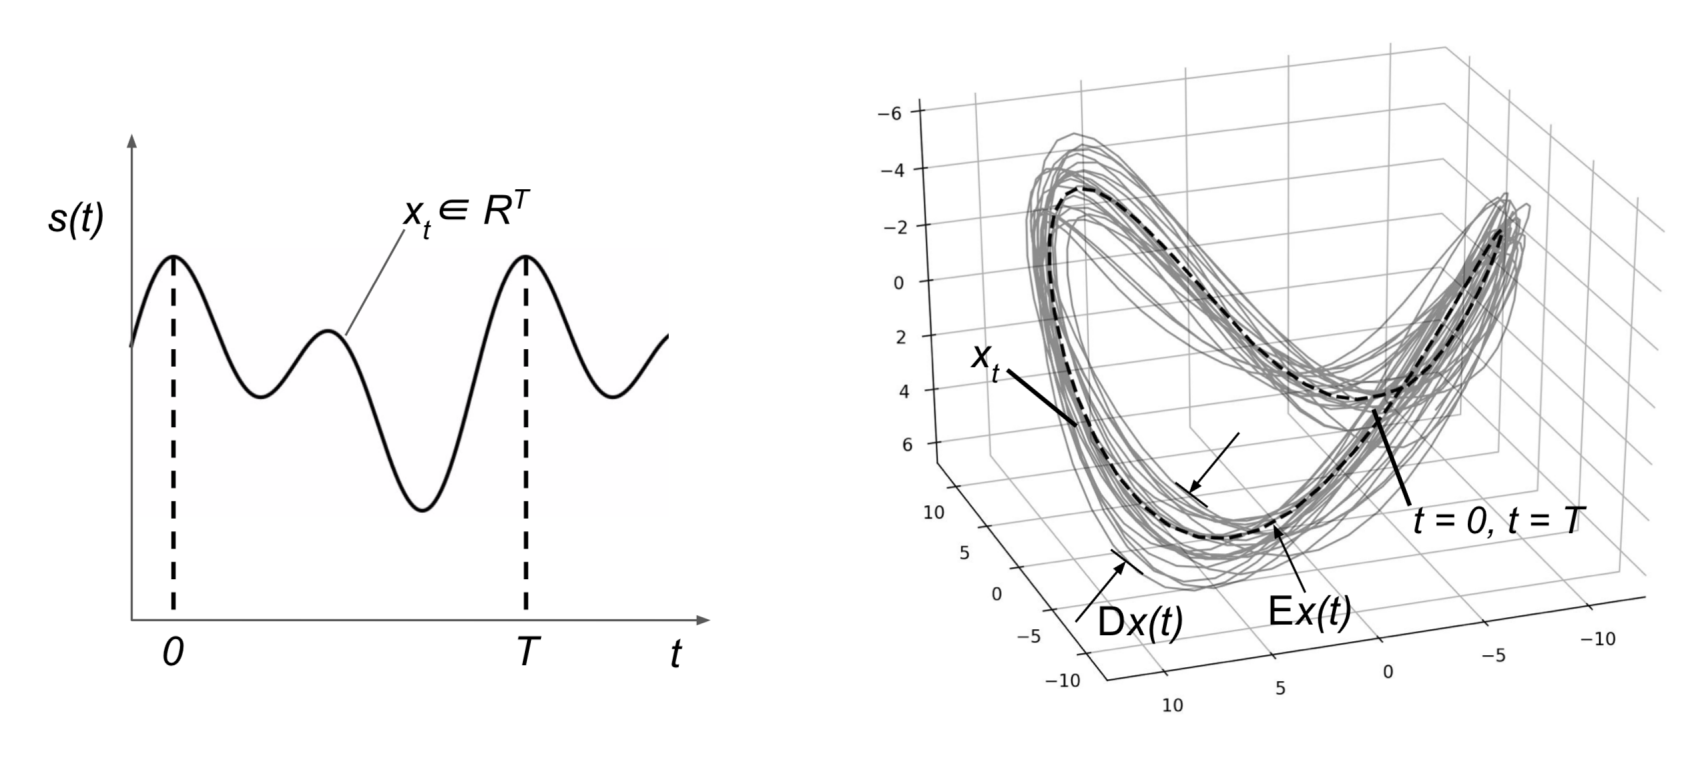
\includegraphics[width=0.9\textwidth, keepaspectratio]{../../figs/phase_traj.png}
		\caption{Time series's phase trajectory visualization }\label{pic:phase_traj}
	\end{figure}
	
	The rest of the paper covers the theory and application of our method on the real data. Firstly, the mathematical model will be introduced and basis search in the signal space problem will be stated and resolved. These results will enable us to propose a way of decomposing the signals and make a forecast. Simultaneously, features of obtained solutions will be examined and result in two theorems. Finally, tSSA and mentioned methods will be applied on two datasets: electricity consumption and meteorology observations. We will obtain signal's predictions and additive decompositions. For the latter a special metric will be formulated. All results will be backed with figures and discussion.
	
	\section{Problem statement}\label{sec:problem_statement}
	
	Let us have observed multidimensional time series $ \{x_i(t)\}_{i=1}^m $ generated by some \emph{dynamical system} $ f $. By that we mean a law of coordinates $ \mathbf{y} \in X $ evolution in discrete time:
	
	\begin{gather*}
		\mathbf{y}(t + 1) = f(\mathbf{y}(t)), \ t \in \mathbb{N} \\
		\mathbf{y}(0) = \mathbf{y}_0
	\end{gather*}
	
	Here $ X $ is generally a high dimensional smooth manifold. Then, each trajectory of the system spawns our signals through unknown mapping $ \boldsymbol{\phi}: X \to \mathbb{R}^m $:
	
	\begin{equation*}
		\boldsymbol{\phi}(\mathbf{y}(t)) = \mathbf{x}_t \Leftrightarrow \begin{cases}
			\phi_1(\mathbf{y}(t)) = x_1(t) \\
			\ldots \\
			\phi_m(\mathbf{y}(t)) = x_m(t) \\
		\end{cases}
	\end{equation*}
	
	After that, it is hypothesized that trajectories $ \mathbf{y}(t) $ actually lie in a smaller dimension manifold $ M \subset X $. So now we should find an embedding of $ M $ into $ \mathbb{R}^{L} $ for some $ L $ and discover a basis in the image of the embedding. Having done that, we will obtain characterization of the initial system in terms of the standard linear space. The same will be equally applied to all $ x_i(t) $.
	
	\subsection*{One signal case}
	
	Our future approach roots from SSA method and Takens's theorem~\cite{citeulike:2735031}. Let's describe it in short. The theorem provides a solution for the stated problem in case of single series: any point $ \mathbf{y}(t) \in M $ we associate with the following vector:
	
	\[
	( \, \boldsymbol{\phi} \circ f^{t - L + 1}(\mathbf{y}(t)), \ldots , \boldsymbol{\phi} \circ f(\mathbf{y}(t)), \boldsymbol{\phi} \circ \mathbf{y}(t) \,)^{\mathsf{T}} = (x(t - L + 1), \ldots , x(t-1), x(t))^{\mathsf{T}}
	\] 
	
	It is called \emph{delay vector} in time $ t $ and denoted as $ \delayV{t} $. Their dimensionality $ L $ should satisfy $ L > 2 \cdot \dim(M) $. Function $ \phi(\cdot) $ should also meet some regularity conditions which are assumed to be fulfilled.
	
	So, with signal $ x(t) $ of length $ N $ we build $ N - L + 1 $ delay vectors. Corresponding embedding space $ \text{Lin}(\{\delayV{t}\}) $, so called \emph{signal subspace}, must be low dimensional, meaning $ \text{Lin}(\{\delayV{t}\}) \subset \mathbb{R}^L $. Orthonormed basis here is a SVD's $ U $-component of \emph{trajectory matrix} $ \mathbf{H}_x $ which is build from delay vectors:
	
	\[
		\mathbf{H}_x = [ \delayV{1} \ldots  \delayV{N - L + 1}]
	\]
	
	\subsection*{Series interconnection and tSSA method}\label{sec:tssa_method}
	
	Теперь обобщим данный подход на несколько временных рядов.
	
	Now let's generalize previous results for the multiple series.
	
	\begin{figure}[h]
		\centering
		\subfigure{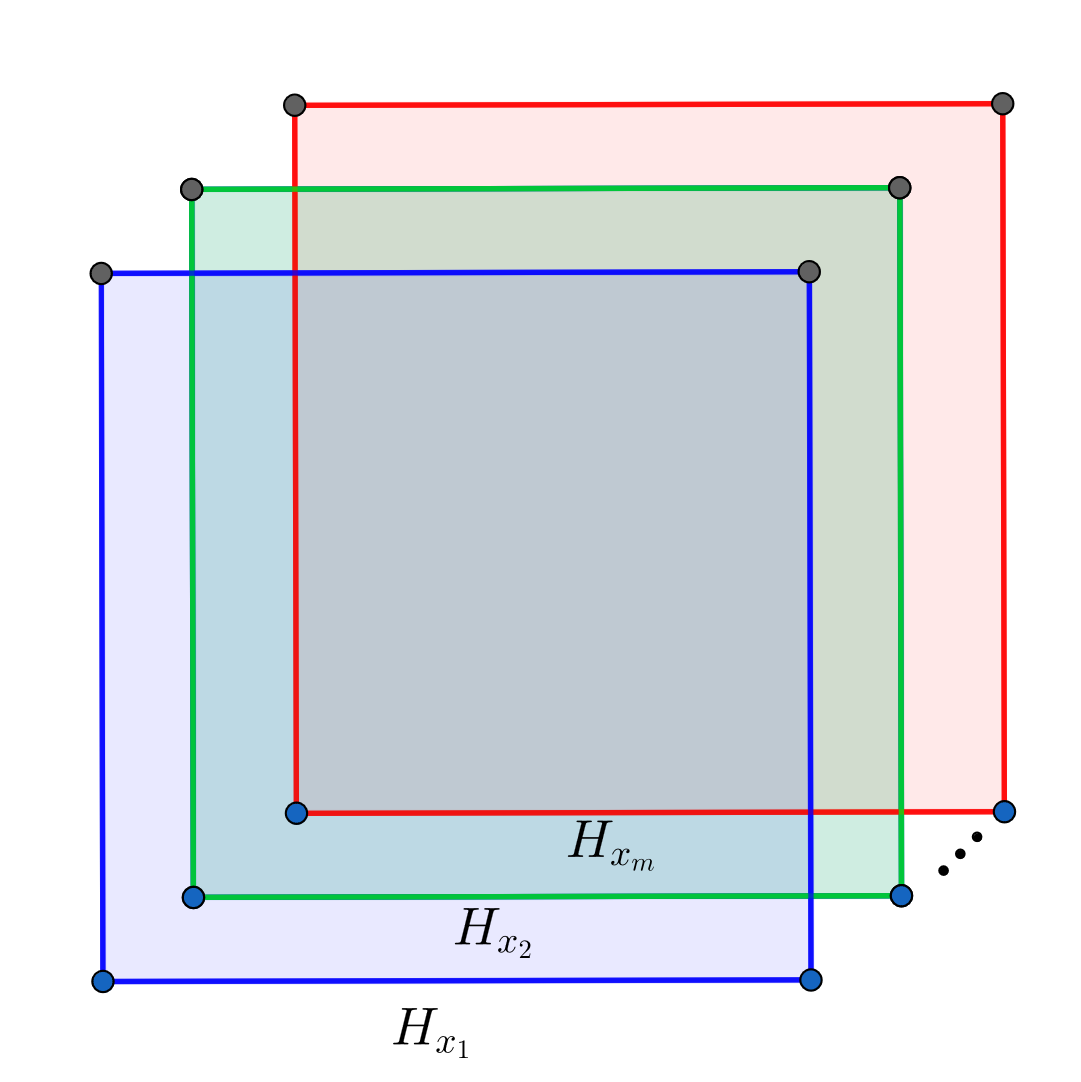
\includegraphics[width=0.4\textwidth, keepaspectratio]{../../figs/Trajectory_Tensor_1}}
		\subfigure{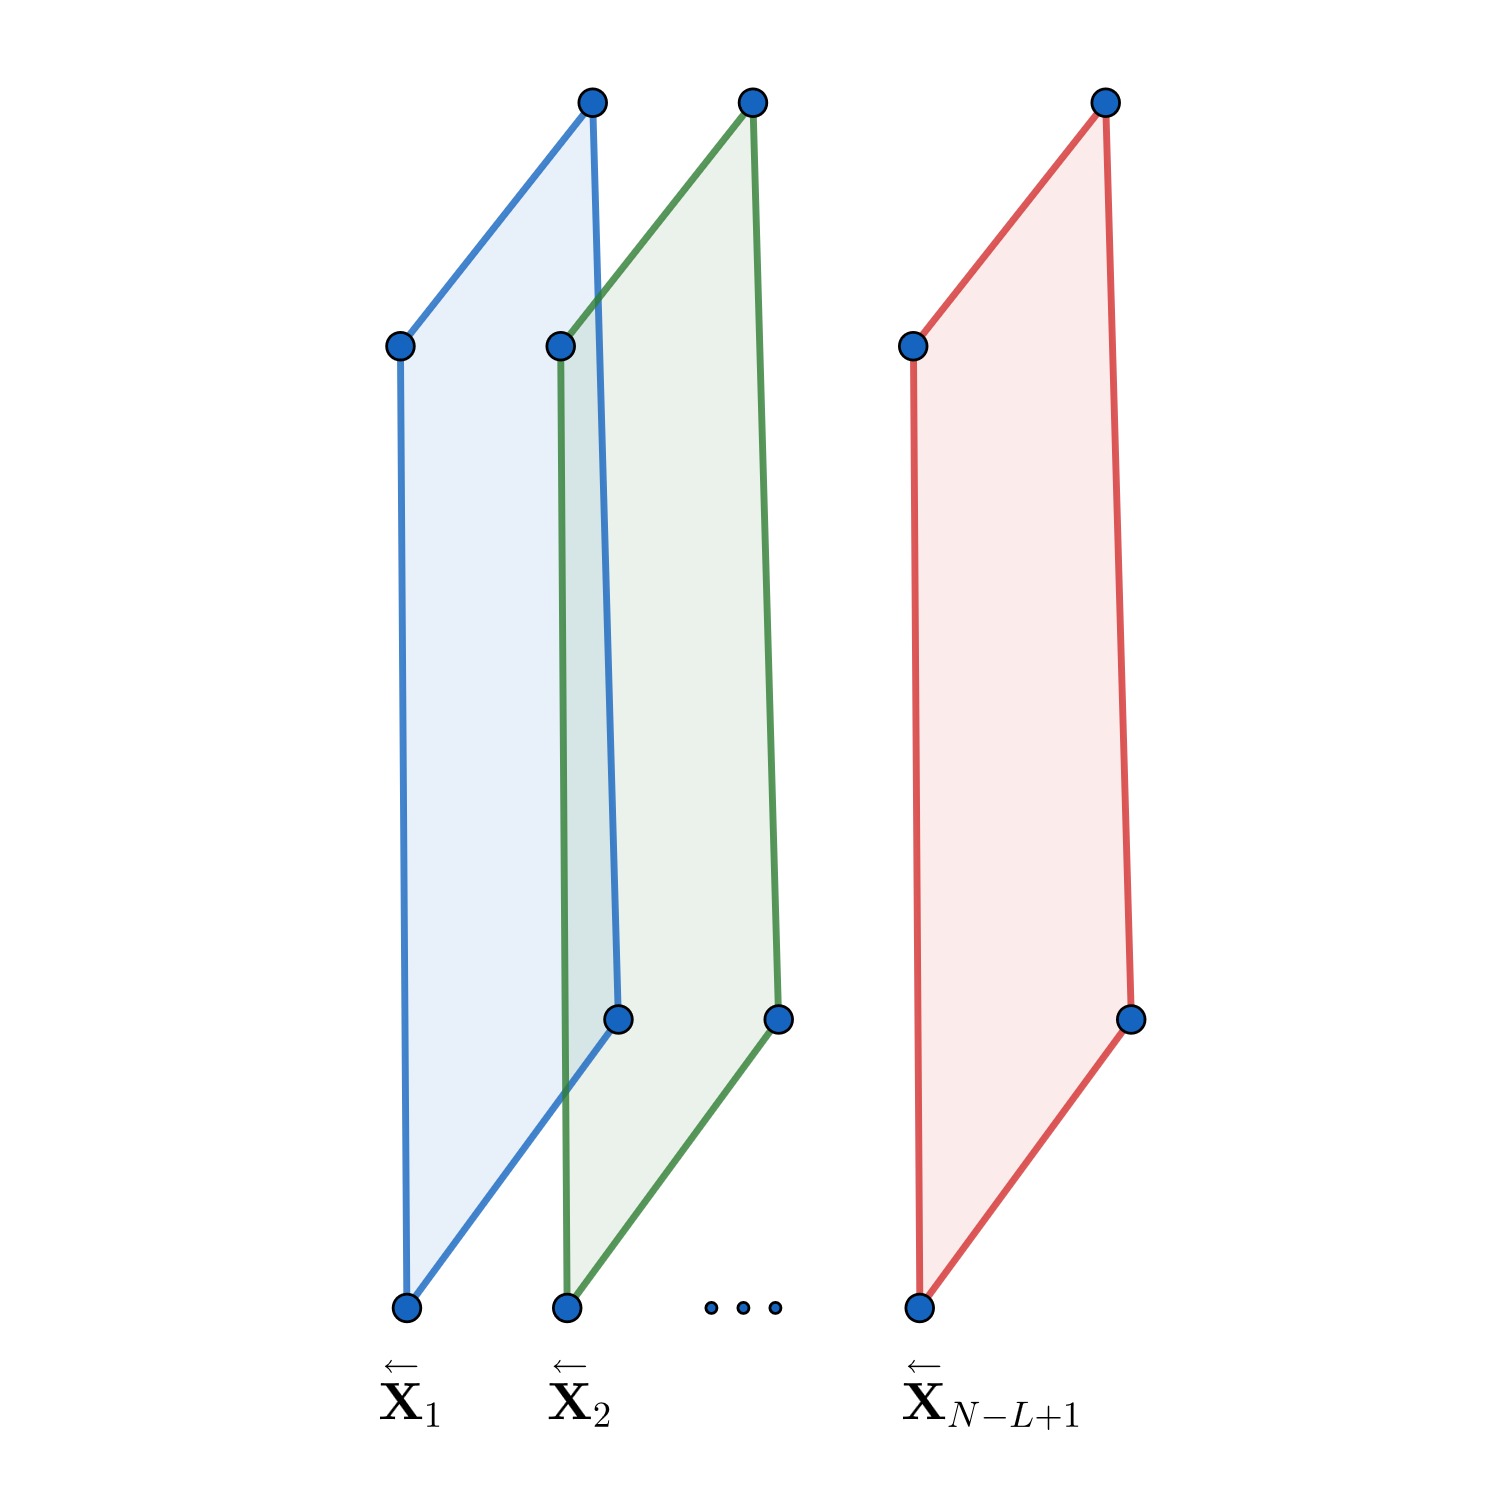
\includegraphics[width=0.4\textwidth, keepaspectratio]{../../figs/Trajectory_Tensor_2}}
		
		\caption{Two views on trajectory tensor. The left is in terms of signals' trajectory matrices $ \{x_i(t)\}_{i=1}^m $. The right is in terms of delay matrices.}\label{pic:traj_tensor}
	\end{figure}
	
	In this case $ \boldsymbol{\phi}(\cdot) $ is multidimensional. So instead of the single delay vector we should consider their set for all $ m $ signals in time $ t $. That means the embedding image now contains so called \emph{delay matrices} $ ( \delayV{1_t} \ldots \delayV{m_t} ) := \delayM{t} $. Next, instead of trajectory matrix we should introduce \textit{trajectory tensor} $ \mathbf{T} $. It is constructed  by putting delay matrices along the second dimension of the tensor, fig. \ref{pic:traj_tensor} (left). This procedure is equivalent to the one for $ \mathbf{H}_x $. But our tensor has an important property: $ \mathbf{T} $ can also be built as an alignment of signals' trajectory matrices $ \mathbf{H}_{x_i} $ along the third dimension, fig. \ref{pic:traj_tensor} (right).
	
	Then, reasoning analogues to the one signal case we obtain \emph{signals' set subspace} as a linear span of delay matrices. But we were supposed to built the subspace for each signal individually.
	
	It's time to give a definition for signals' interrelation in our model's scope.
	
	\begin{Def}		
		We call a set of time series \emph{interconnected} if they all share the common subspace with the same basis.
	\end{Def}
	
	Now we are ready to find this shared elements for signals. Note that to do so we just need to decompose each signal's trajectory matrix through the same set of factors. Finally, let's apply CPD to our trajectory tensor and have a look at its slices by third dimension.
	
	\begin{equation}\label{eq:tSSA_decomp}
		\mathbf{T} = \sum\limits_{i = 1}^{r} \mathbf{a}_i \otimes \mathbf{b}_i \otimes \mathbf{c}_i \Leftrightarrow \begin{cases}
			\mathbf{H}_{x_1} = \sum\limits^{r} \boldsymbol{\sigma}_{x_1}(i) \cdot \mathbf{a}_i  \mathbf{b}_i^{\mathsf{T}}  \\
			\mathbf{H}_{x_2} = \sum\limits^{r} \boldsymbol{\sigma}_{x_2}(i) \cdot \mathbf{a}_i  \mathbf{b}_i^{\mathsf{T}} \\
			\ldots \\
			\mathbf{H}_{x_m} = \sum\limits^{r} \boldsymbol{\sigma}_{x_m}(i) \cdot \mathbf{a}_i  \mathbf{b}_i^{\mathsf{T}} 
		\end{cases}
	\end{equation}
	
	What have we got? CPD is defined by tensor rank $ r $ and a set of vectors which we can pack in matrices: $ A = [\mathbf{a}_1 \ldots \mathbf{a}_r]; B = [\mathbf{b}_1 \ldots \mathbf{b}_r]; C = [\mathbf{c}_1 \ldots \mathbf{c}_r] $. Row $ k $ of matrix $ C $ is denoted as $ \boldsymbol{\sigma}_{x_k} $. It has the sense of singular values but can be negative.
	
	After, from CPD definition as a (\ref{eq:tSSA_decomp}) kind decomposition with minimal $ r $ we can derive that $ A, B, C $ are full-rank matrices. So, signals' shared subspace is  $ \text{Lin}(\{\mathbf{a}_i\}) $ with unified basis $ \{\mathbf{a}_i\}_{i = 1}^r $ which is not orthonormed in general. Then, back in the problem statement we assumed dimensionality of the embedding to be rather small. Therefore relation $ r \ll L $ should be true.
	
	Lastly, let's note that \emph{rows} of $ \mathbf{H}_{x_k} $ are also delay vectors but have another dimension of $ N - L + 1 $. So the shared subspace for them would be $ \text{Lin}(\{\mathbf{b}_i\}) $. This result proves our approach to be consistent with choice of $ \delayV{k_t} $. As a remark, mSSA lacks such feature.
	
	What to the signals' link, it is regulated by $ \boldsymbol{\sigma}_{x_k} $. For instance, if all the rows have zero elements in non-overlapping positions then our built subspace breaks down into a direct sum of individual signal's subspaces. It is total link absence case. The exact opposite situation is when $ \boldsymbol{\sigma}_{x_k} $ are non-zero for all series.
	
	\subsection*{Time series decomposition}\label{sec:decomposition}
	
	We can break series into several components using the conception: \emph{decomposition of trajectory matrix $ \mathbf{H}_{x_k} $ defines decomposition of related signal}. Its first part implies representation of $ \mathbf{H}_{x_k} $ as a sum of factors (\ref{eq:tSSA_decomp}). This technique comes from SSA. Because all matrices are similarly decomposed, we can focus on the task for a single series.
	
	Besides, we should point out the main feature of trajectory matrices --- \emph{hankelness}. That simply means equal elements along each anti-diagonal. Every series of length $ N $ bijectionly corresponds to hankel matrix of size $ L \times (N - L + 1) $.
	
	Now, decomposition procedure is following: we assume factors of $ \mathbf{H}_{x_k} $ to be able to pack in $ s $ groups in a special way. That means if we sum all factors within each group the result matrices $ C_1, \ldots, C_s $ will be hankel. This situation would perfectly correspond to representation of $ x_k(t) $ as a sum of $ s $ signals. Unfortunately, it is almost infeasible even with trivial series \cite{ecfb9dc578be43ae9ee8fc88b8ff9151}, so every $ C_i $ should be additionally \emph{hankelized}. This operation average each matrix's anti-diagonal so it becomes hankel. Let's denote the operator as $ \text{Hankel}(\cdot) $. 
	
	The whole algorithm can be written as a chain of identical expressions:
	
	\begin{multline}\label{eq:decomp_method_ideal}
		\underline{\mathbf{H}_{x_k}} \overset{1}{=} \sum\limits_{i = 1}^{r} \boldsymbol{\sigma}_{x_k}(i) \cdot \mathbf{a}_i  \mathbf{b}_i^{\mathsf{T}} \overset{2}{=} \sum\limits_{i \in \mathbb{I}_1} \boldsymbol{\sigma}_{x_k}(i) \cdot \mathbf{a}_i  \mathbf{b}_i^{\mathsf{T}} + \ldots + \sum\limits_{i \in \mathbb{I}_s} \boldsymbol{\sigma}_{x_k}(i) \cdot \mathbf{a}_i  \mathbf{b}_i^{\mathsf{T}} \overset{3}{=} \\ \overset{3}{=} C_1 + \ldots + C_s \overset{4}{=} \underline{\text{Hankel}(C_1) + \ldots + \text{Hankel}(C_s)}  \Leftrightarrow x_k(t) = c_1(t) + \ldots c_s(t)
	\end{multline}
	
	Here $ \mathbb{I}_1 \sqcup \ldots \sqcup \mathbb{I}_s = \{1, \ldots, r\} $ --- chosen groups of indices. Actually, the forth equality needs some extra validation. To make it, first consider hankel operator's property:
	
	\begin{Lem}
		$ \text{Hankel}(\cdot) $ operator is linear.
	\end{Lem}
	
	\begin{proof}		
		Having matrices $ A $ and $ B $ with the same size, let's look at their elements from one anti-diagonal $ a_1, \ldots, a_n $ and $ b_1, \ldots, b_n $. Then this anti-diagonal in $ \text{Hankel}(A + B) $ is written as $ \dfrac{1}{n} \sum\limits^n (a_i + b_i) = \dfrac{1}{n} \sum\limits^n a_i + \dfrac{1}{n} \sum\limits^n b_i $, resulting in a sum of  $ \text{Hankel}(A) $ and $ \text{Hankel}(B) $ anti-diagonals.
		
		Secondly, having a scalar $ \alpha $ it is also trivial that $ \dfrac{1}{n} \sum\limits^n \alpha \cdot a_i = \alpha \dfrac{1}{n} \sum\limits^n a_i $. Then we finally derive $ \text{Hankel}(\alpha A) = \alpha \text{Hankel}(A) $.
	\end{proof}
	
	Returning to the forth equality in (\ref{eq:decomp_method_ideal}), we can combine this lemma and the fact that $ \mathbf{H}_{x_k} $ is itself hankel to get a complete justification. This outputs in the correctness of series decomposition procedure for any chosen grouping of factors.
	
	\subsection*{Optimal decomposition and its computational complexity}\label{sec:optimal_decomp}
	
	Even though decomposition algorithm from the previous subsection is correct for any factors' grouping we might want to find the best one. This would mean every $ C_i $ to be as close to hankel matrix as possible. Having that the formulated decomposition concept would be fully accomplished and signal's components could be naturally extracted. Let's rewrite it as some optimization task.
	
	Consider the first equality from (\ref{eq:decomp_method_ideal}) and itself with hankel operator applied. Also recall that $ \mathbf{H}_{x_k} $ is hankel. We obtain:
	
	\begin{equation*}
		\begin{cases*}
			\mathbf{H}_{x_k} = \sum\limits_{i = 1}^{r} \boldsymbol{\sigma}_{x_k}(i) \cdot \mathbf{a}_i  \mathbf{b}_i^{\mathsf{T}} \\
			\mathbf{H}_{x_k} = \sum\limits_{i = 1}^{r} Hankel(\boldsymbol{\sigma}_{x_k}(i) \cdot \mathbf{a}_i  \mathbf{b}_i^{\mathsf{T}})
		\end{cases*}
	\end{equation*}
	
	Subtract the second equation from the first and denote $ H_i = \boldsymbol{\sigma}_{x_k}(i) \cdot \mathbf{a}_i  \mathbf{b}_i^{\mathsf{T}} - Hankel(\boldsymbol{\sigma}_{x_k}(i) \cdot \mathbf{a}_i  \mathbf{b}_i^{\mathsf{T}}) $. This can be sensed as residual between initial matrix and its hankelized version. So we have:
	
	\begin{equation}\label{eq:residuals_equation}
		H_1 + \ldots + H_r = 0 \Leftrightarrow H_r = - \sum\limits_{j = 1}^{r - 1} H_j
	\end{equation}
	
	What we have done is reformulated condition on $ C_i $ to be hankel in terms of residual matrices summing into zero inside groups: $ \sum_{k \in \mathbb{I}_i} H_k = 0, \  \forall i \in 1, \ldots, s $.
	
	Now let's simplify our case by decreasing the number of desired components from $ s $ to two. If we worked out the easier problem we could consecutively dissect components into two more and have as much of them as we want.  
	
	Next, (\ref{eq:residuals_equation}) shows all residual matrices already total in zero. Therefore we can discard, for example, $ H_r $ as group for it would be defined automatically if having groups for the rest factors. Let's introduce indicator-variables $ \beta_j \in \{0, 1\} $ showing in what of two groups factor $ j $ lies.
	
	Finally, we assume all $ H_i $ to be non-zero; otherwise we already have needed dissection. This last condition implies each group to have at least two residual matrices. So we are ready for the optimal decomposition problem statement:
	
	\begin{equation}
		\begin{cases*}
			\sum\limits_{j = 1}^{r - 1} \beta_j H_j = 0 \\
			\beta_j \in \{0, 1\}, \ \forall j \in 1, \ldots, r \\
			\sum\limits_{i = 1}^{r - 1} \beta_j \ge 2
		\end{cases*}
	\end{equation}
	
	To rewrite it in a more familiar way let's vectorize each $ H_i $ and put resulting vectors in a matrix $ \Lambda $. Furthermore, introduce $ \boldsymbol{\beta} = (\beta_1 \ldots \beta_{r-1}) $. Then, recall from previous subsection that it is highly unlikely for residual matrices to total in zero within all groups. The most we can is to make them as close to zero as possible. So restated problem:
	
	\begin{equation}\label{eq:decomp_search_final}
		\begin{cases*}
			\lVert \Lambda \boldsymbol{\beta} \rVert \to \underset{\boldsymbol{\beta}}{\min} \\
			\beta_j \in \{0, 1\}, \ \forall j \in 1, \ldots, r \\
			\sum\limits_{i = 1}^{r - 1} \beta_j \ge 2
		\end{cases*}
	\end{equation}
	
	Let's declare solution of this task \emph{optimal series decomposition}. It is represented as Integer Least Squares problem which is proved to be NP-hard~\cite{van1981another}. In short, subsection's output is:
	
	\begin{Th}
		Optimal series decomposition as special grouping of trajectory matrix's factors search is NP-hard.
	\end{Th}
	
	In spite of the result, methods and heuristics exist to reduce ILS to computationally effective objectives~\cite{Grafarend2022}.
	
	\subsection*{Forecasting}\label{sec:tssa_forecast}
	
	In our model prediction making comes down to restoration of delay vectors for every signal in a set. Because we have the shared basis among series $ \{\mathbf{a}_i\}_{i = 1}^r $ we can process them separately. 
	
	If $ \{\mathbf{a}_i\}_{i = 1}^r $ was orthornormal we could inherit SSA prediction technique~\cite{ecfb9dc578be43ae9ee8fc88b8ff9151}. But we don't have this warranty so we are going to adopt it for our case.
	
	Having input series $ x(t) $ we want to forecast it for one step further. Delay vector $ \delayV{N + 1} = (x(N - L) \ldots x(N + 1))^{\mathsf{T}} $, with the last component unknown, belongs to the $ \text{Lin}(\{\mathbf{a}_i\}) $. In terms of full-ranked matrix $ A \in \mathbb{R}^{L \times r} $ (see \hyperref[sec:tssa_method]{Series interconnection and tSSA method}) it can be written as:
	
	\begin{align}\label{eq:main_pred_for_A}
		\delayV{N + 1} = A \boldsymbol{\lambda} &\Leftrightarrow \begin{cases}
			\mathbf{x}_{kn} = A_{kn} \boldsymbol{\lambda}  \\
			x(N + 1) = \mathbf{a}_{pr}^{\mathsf{T}} \boldsymbol{\lambda}
		\end{cases}, \text{ where } \\
		A &= \left( \dfrac{A_{kn}}{\mathbf{a}_{pr}^{\mathsf{T}}} \right) \nonumber \\
		\delayV{N + 1} &= (\mathbf{x}_{kn} \  x(N + 1))^{\mathsf{T}} \nonumber
	\end{align}
	
	Here variable $ \boldsymbol{\lambda} \in \mathbb{R}^r $. Delay vector and matrix are broken into two blocks associated with the \emph{known} and \emph{unknown} part of the series. To make prediction we need to find $ \boldsymbol{\lambda} $ so we focus on the first obtained equation.
	
	The matrix of this linear system $ A_{kn} \in \mathbb{R}^{(L - 1) \times r} $ has a rank at least $ r - 1 $ by construction. But we assume elimination of one row in $ A $ will actually keep the rank full. As experiments show this is not burdensome. After that, we note that the linear system itself is overdetermined due to the model hypothesis $ r \ll L $. Therefore it is reasonable to get solution in a least squares sense: $ \boldsymbol{\lambda} = (A_{kn}^T A_{kn})^{-1} A_{kn}^T \mathbf{x}_{kn} $. In the end, forecast is given by the formula:
	
	\begin{equation}\label{eq:tssa_pred}
		x(N + 1) = \mathbf{a}_{pr}^{\mathsf{T}} (A_{kn}^T A_{kn})^{-1} A_{kn}^T \mathbf{x}_{kn}
	\end{equation}
	
	Here $ \mathbf{a}_{pr}^{\mathsf{T}} (A_{kn}^T A_{kn})^{-1} A_{kn}^T = \mathbf{d}^{\mathsf{T}} $ --- row vector which once computed can be reused to make prediction for arbitrary horizon ahead.
	
	Now let's rewrite (\ref{eq:tssa_pred}) in terms of $ x(t) $:
	
	\begin{equation*}\label{eq:autoregr}
		x(t) = \sum\limits_{i = 1}^{L - 1} d_i \cdot x(t - i)
	\end{equation*}
	
	This expression leads to the final result about the forecast behavior:
	
	\begin{Th}		
		The model of tSSA's forecast is \emph{autoregressive} $ AR(L - 1) $. It is fully characterized by coefficients $ d_i $ found in (\ref{eq:tssa_pred}).
	\end{Th}
	
	\section{Computational experiment}	
	
	\subsection*{Goals and setting}
	
	In the current section we will demonstrate application of our method for decomposition and forecast of multidimensional time series. We will also compare it with other models: mSSA, VAR, RNN. The latter two are only able for prediction. The mSSA has a lot in common with our approach and is valid for both tasks.
	
	To measure quality of the decomposition we need special metrics:
	
	\begin{Def}
		\emph{Absolute hankel error} of matrix M is 
		
		\[
		\text{AHE} = \lVert M - \text{Hankel}(M) \rVert_2
		\] 
		
	\end{Def}	
	
	\begin{Def}		
		
		\emph{Relative hankel error} of matrix M is 
		
		\[
		\text{RHE} = \frac{\text{AHE}}{\lVert M \rVert_2} 
		\] 		
		
	\end{Def}
	
	AHE can be imagined as a total standard deviation of matrix's anti-diagonals. RHE is its more convenient modification which will be used further.	
	
	Now, recall that series decomposition on additive components is equivalent to trajectory matrix decomposition, viz. obtaining of matrices $ C_i $ (see \hyperref[sec:decomposition]{Time series decomposition}). The RHE will be calculated for them as well as mean RHE for every series in a set --- $ \overline{\text{RHE}}_{ts} $ and the mean among all series --- $ \overline{\text{RHE}} $. 
	
	To measure forecast quality we will be using standard metrics: mean squared error $ \text{MSE}_{ts} $ and mean absolute percentage error $ \text{MAPE}_{ts} $. Their averaging for all series are denoted as $ \overline{\text{MSE}} $ and $ \overline{\text{MAPE}} $.
	
	Two sets of data will be involved. First, electricity consumption paired with its generation price (fig. \ref{fig:electr_data}). Second, three series describing weather conditions in Berlin from 1980 to 1990: temperature, precipitation and air pressure (fig. \ref{fig:weather_data}). We assume signals' inter-dependency based on economical/physical reasons as it is important premise for our approach (see \hyperref[sec:tssa_method]{Series interconnection and tSSA method}). Then, individual series has a length $ \approx 3 \cdot 10^3 $ where last $ 20\% $ are deferred test samples for prediction evaluation.
	
	\begin{figure}[h]
		\centering
		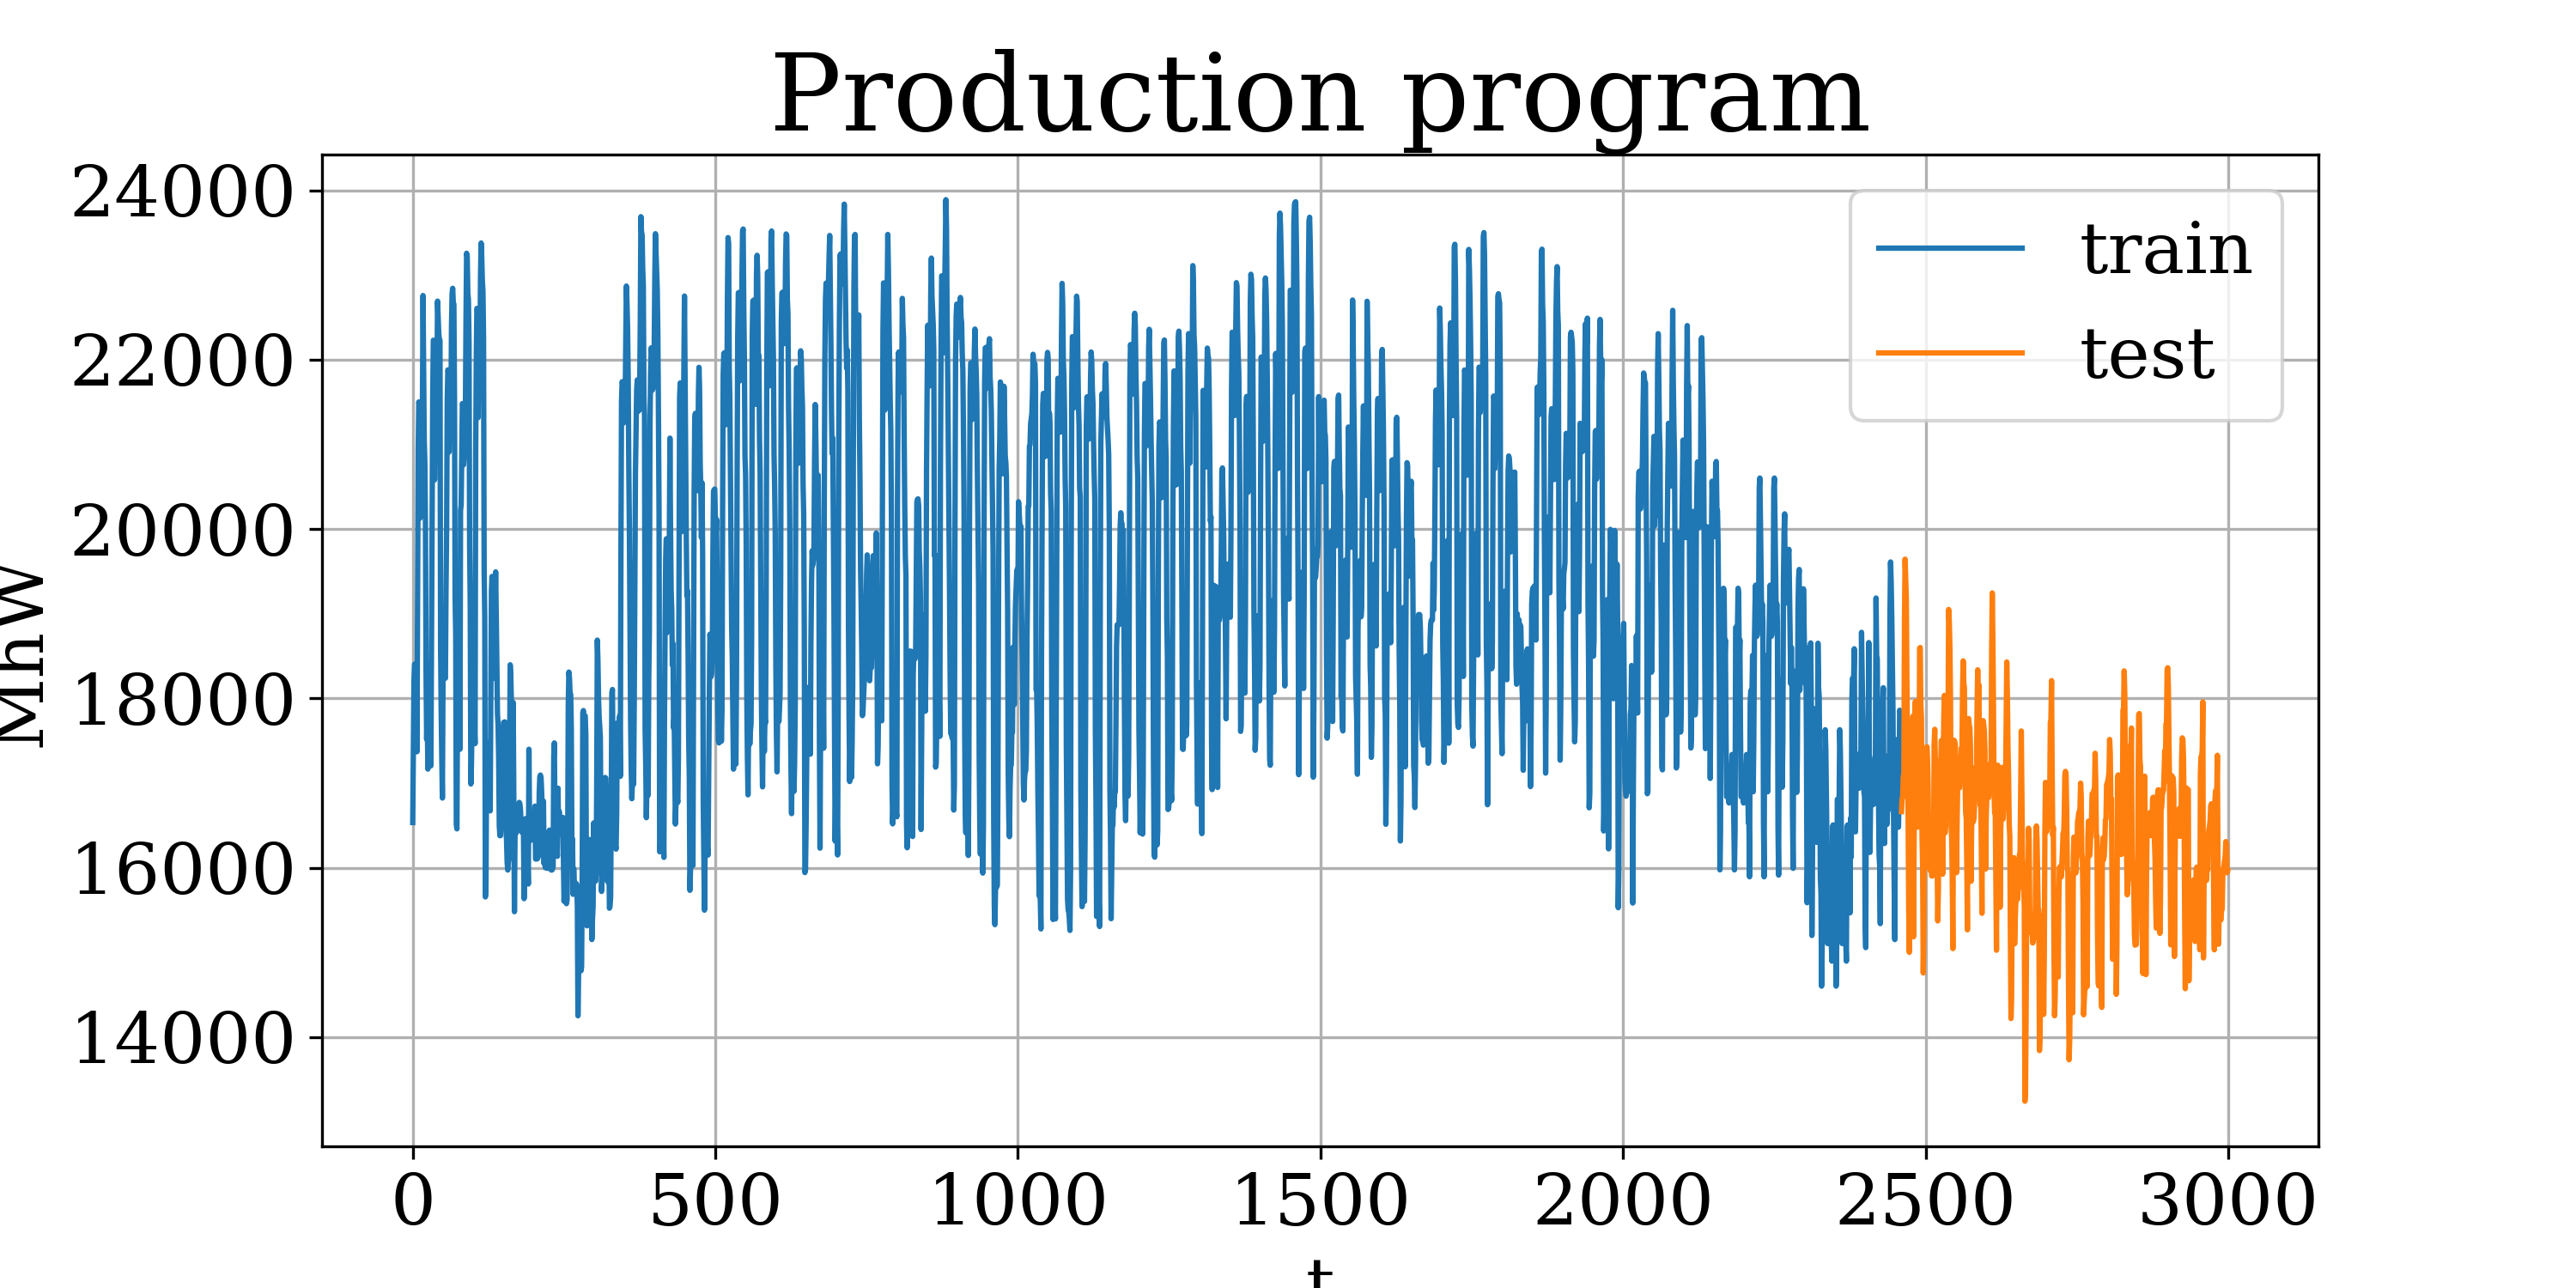
\includegraphics[width=0.48\textwidth, keepaspectratio]{../../figs/Electricity_Production}
		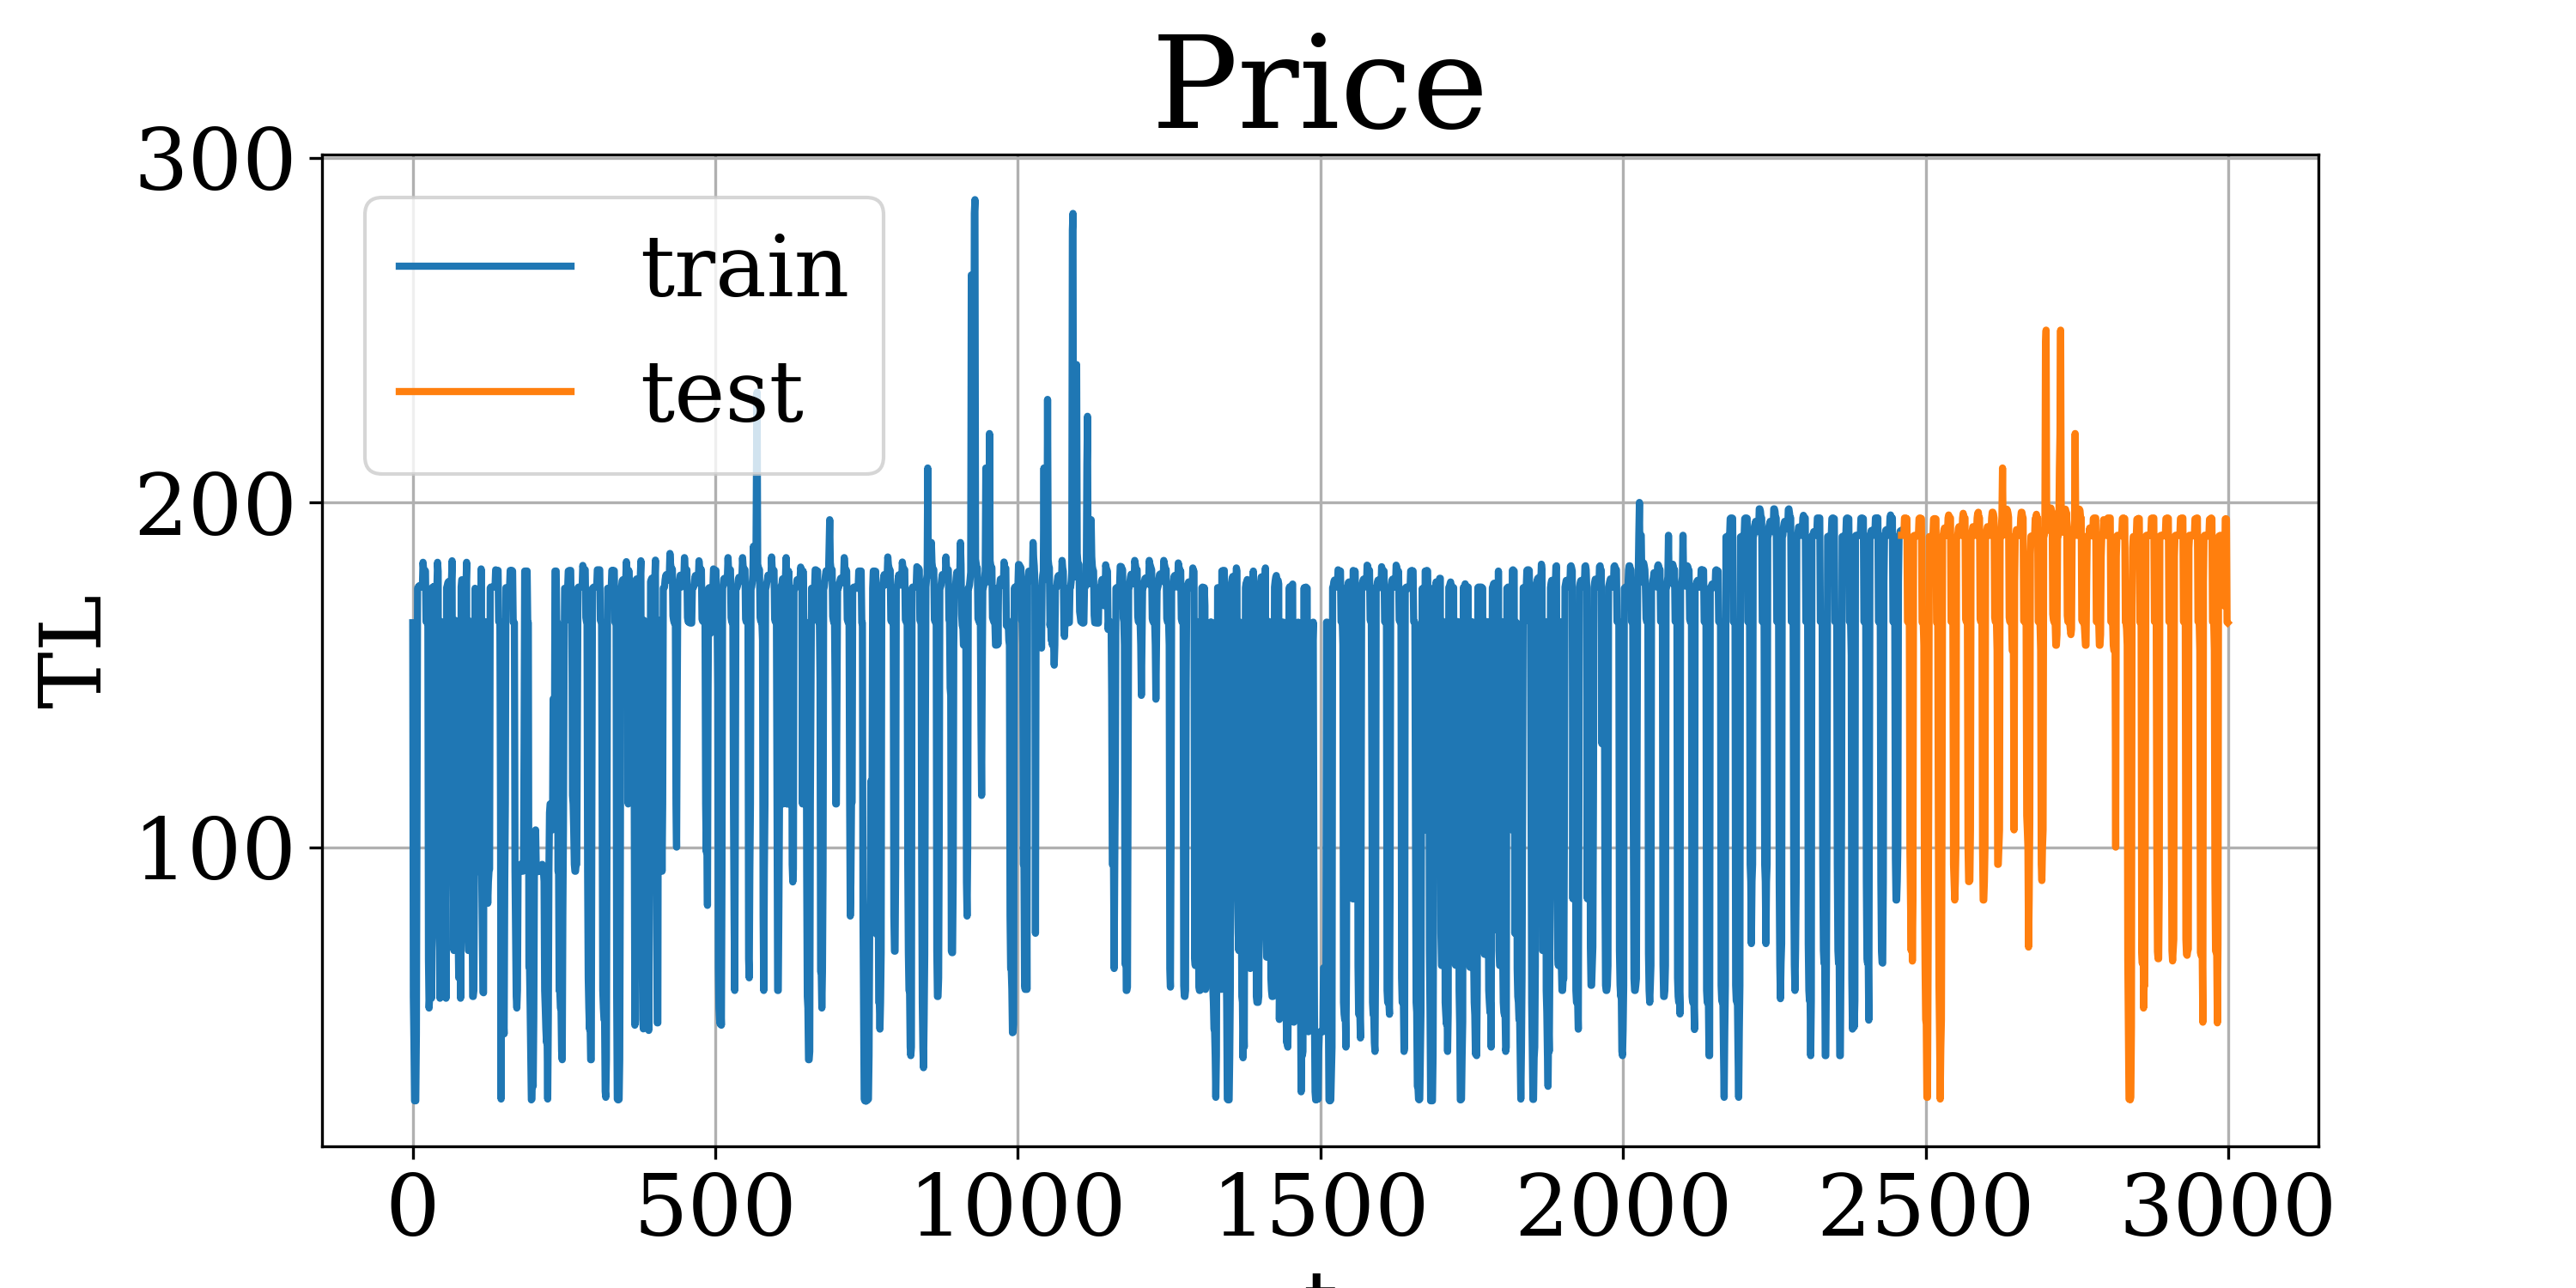
\includegraphics[width=0.48\textwidth, keepaspectratio]{../../figs/Electricity_Price}
		\caption{Time series for electricity consumption and its price}\label{fig:electr_data}
	\end{figure}
	
	\begin{figure}[h]
		\centering
		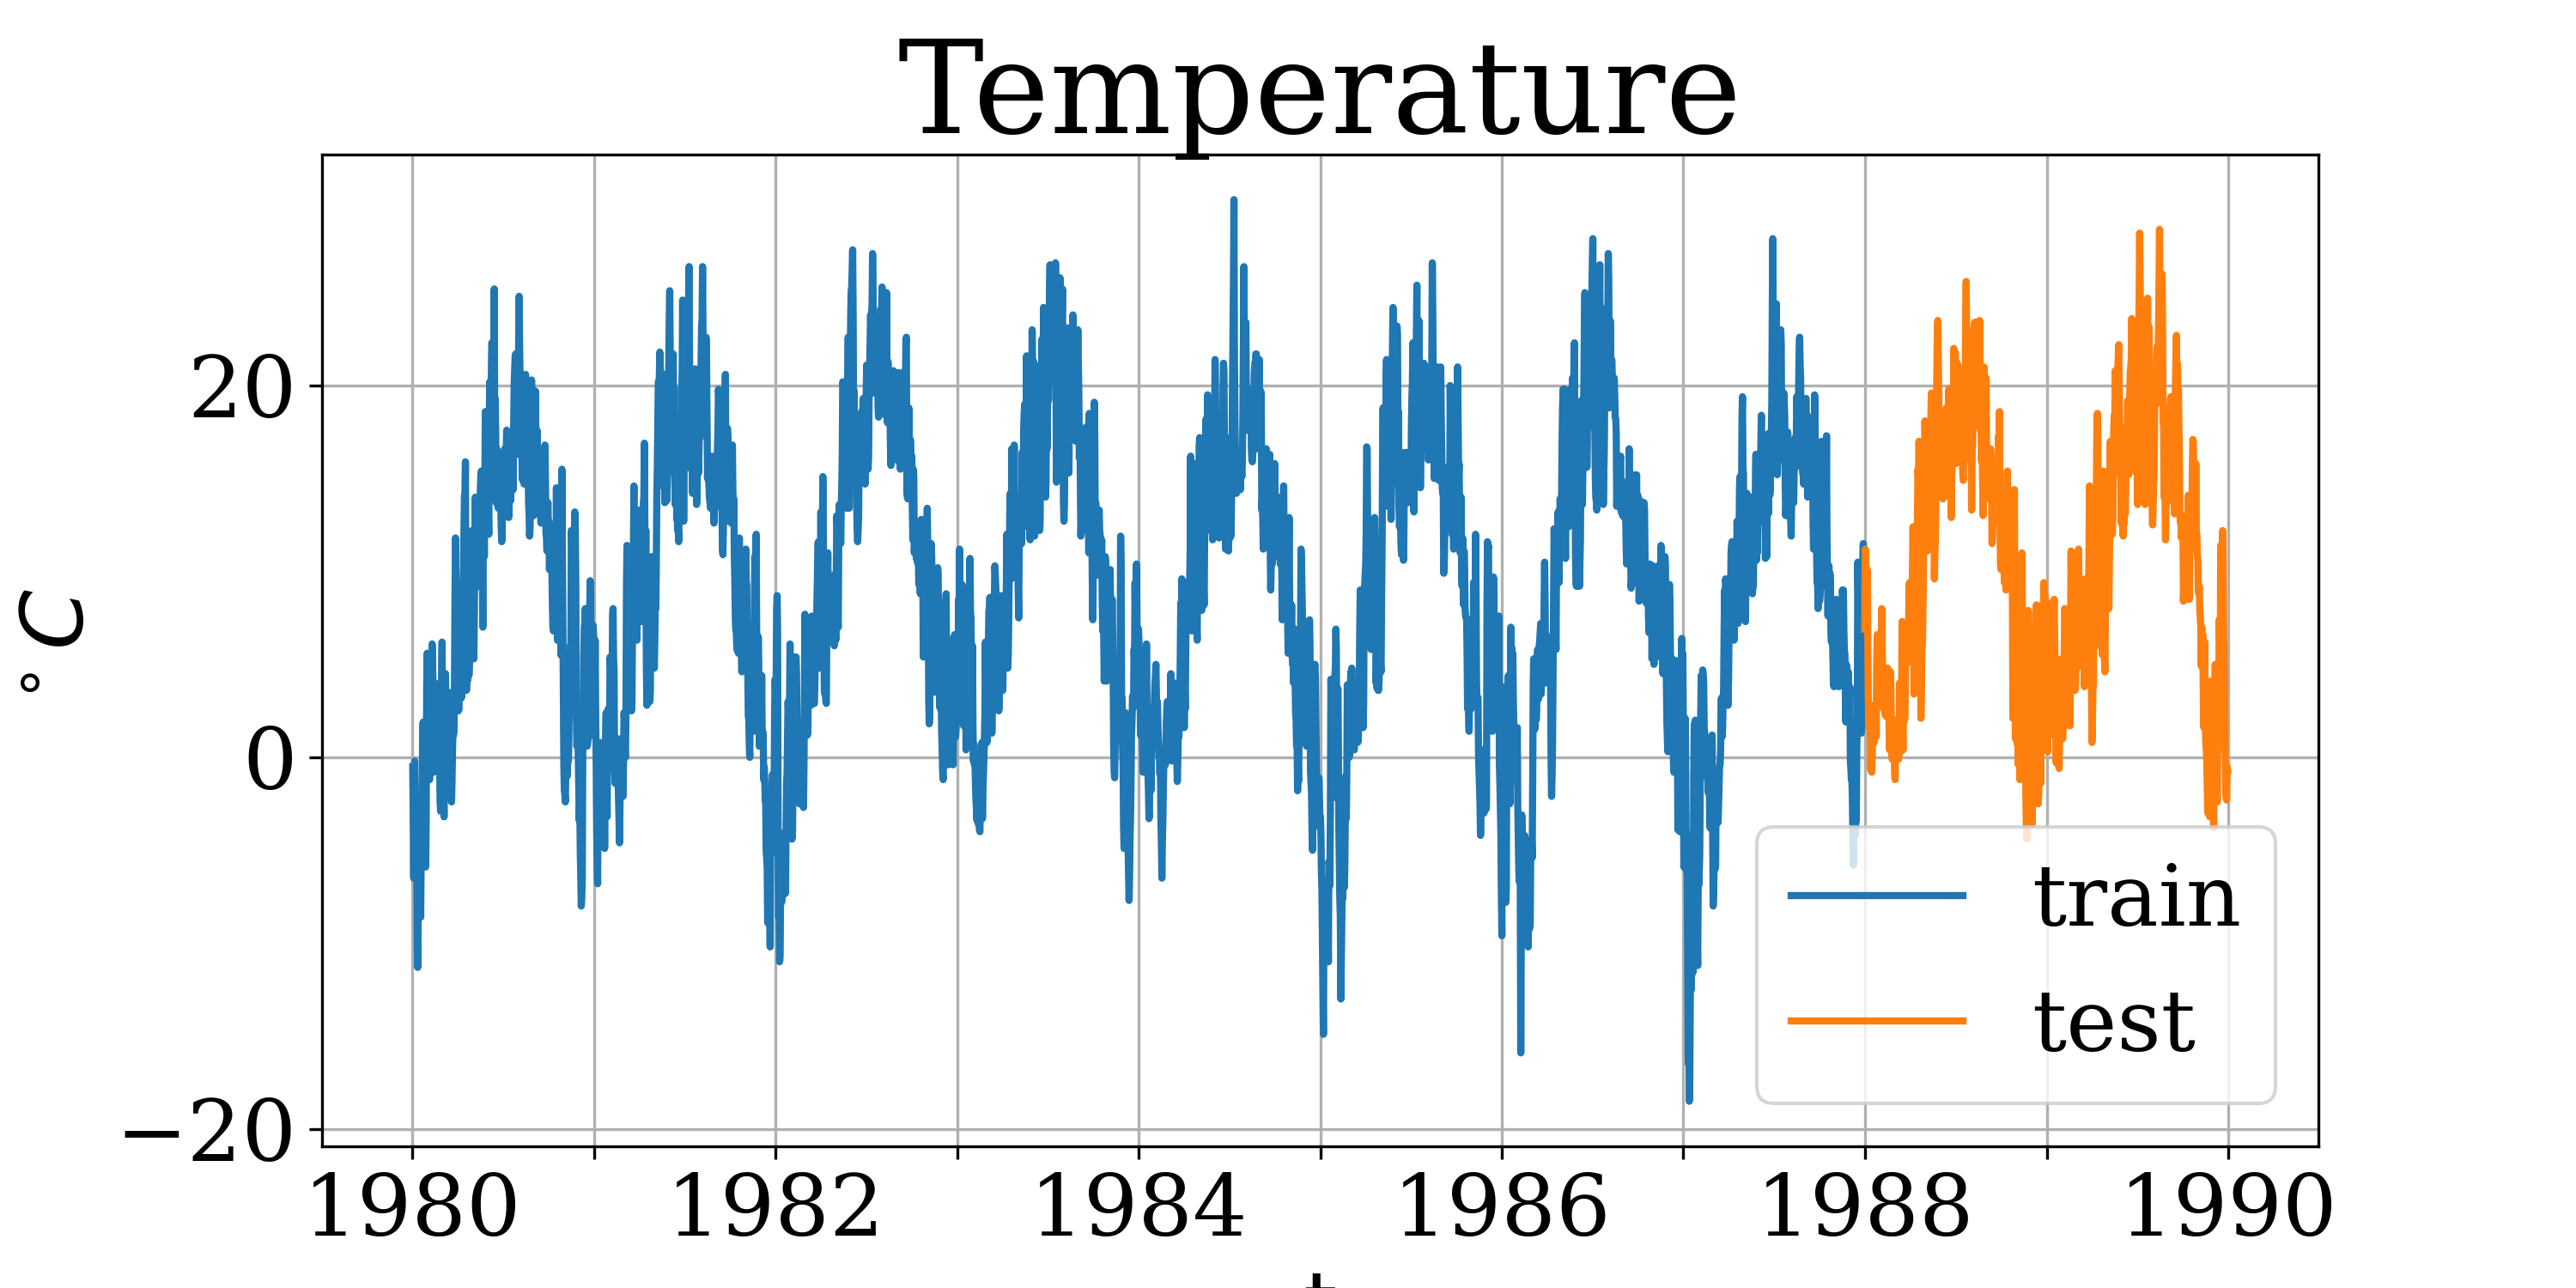
\includegraphics[width=0.48\textwidth, keepaspectratio]{../../figs/Temperature.png}
		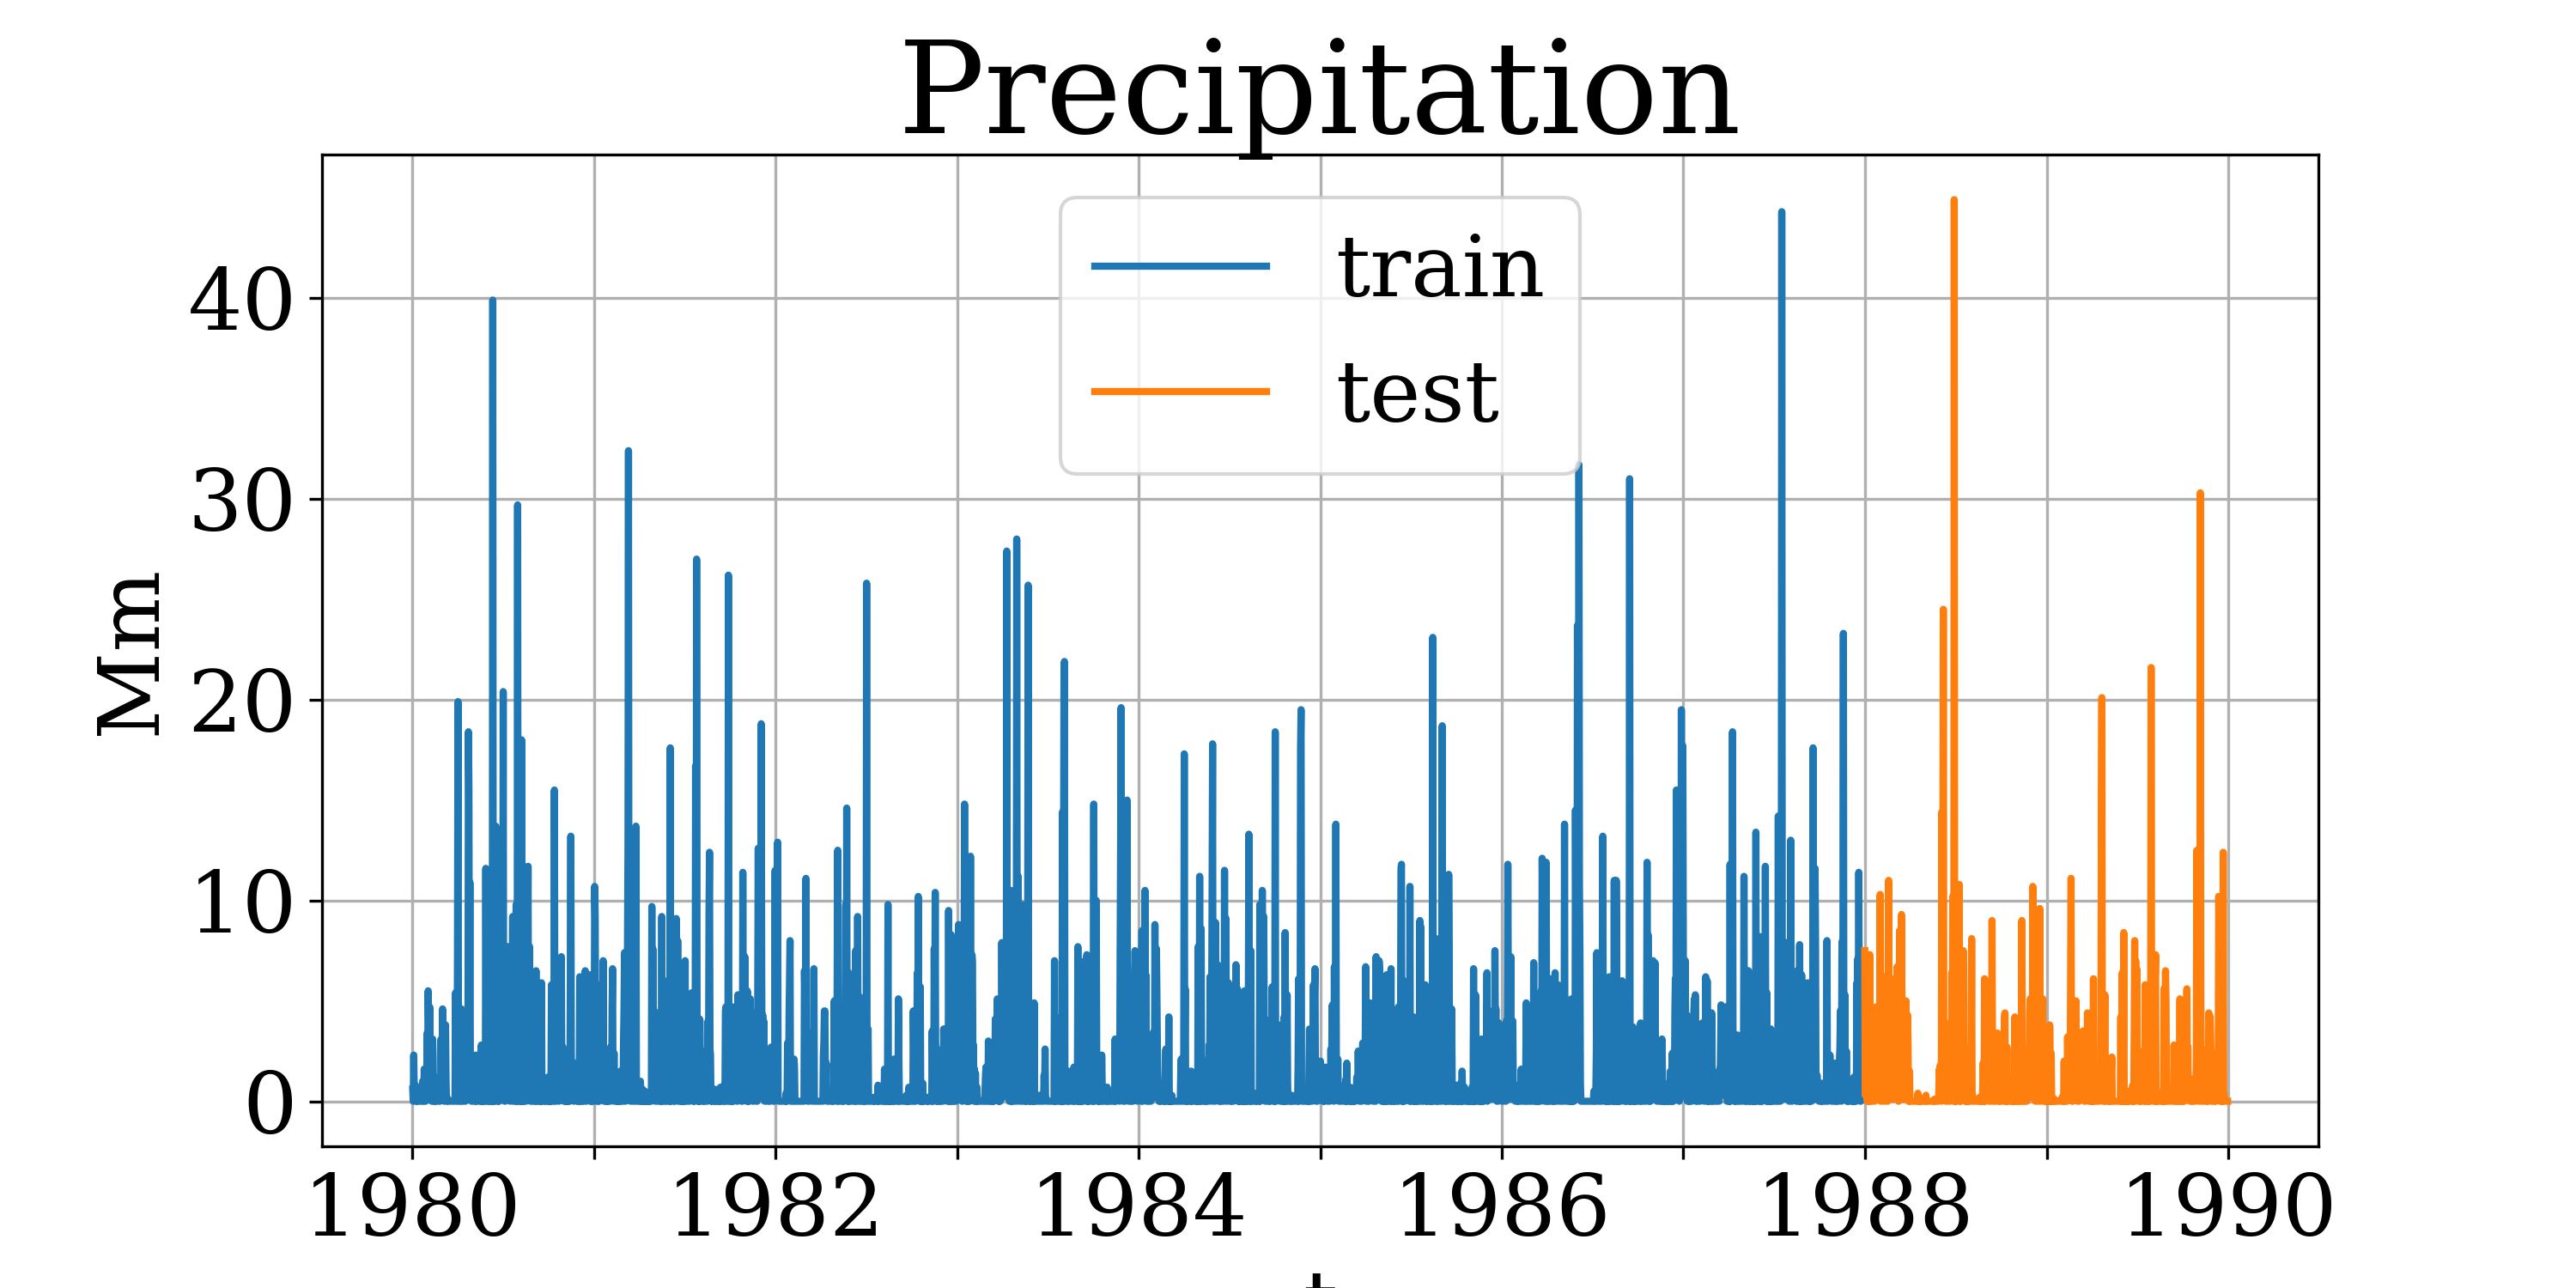
\includegraphics[width=0.48\textwidth, keepaspectratio]{../../figs/Precipitation.png}
		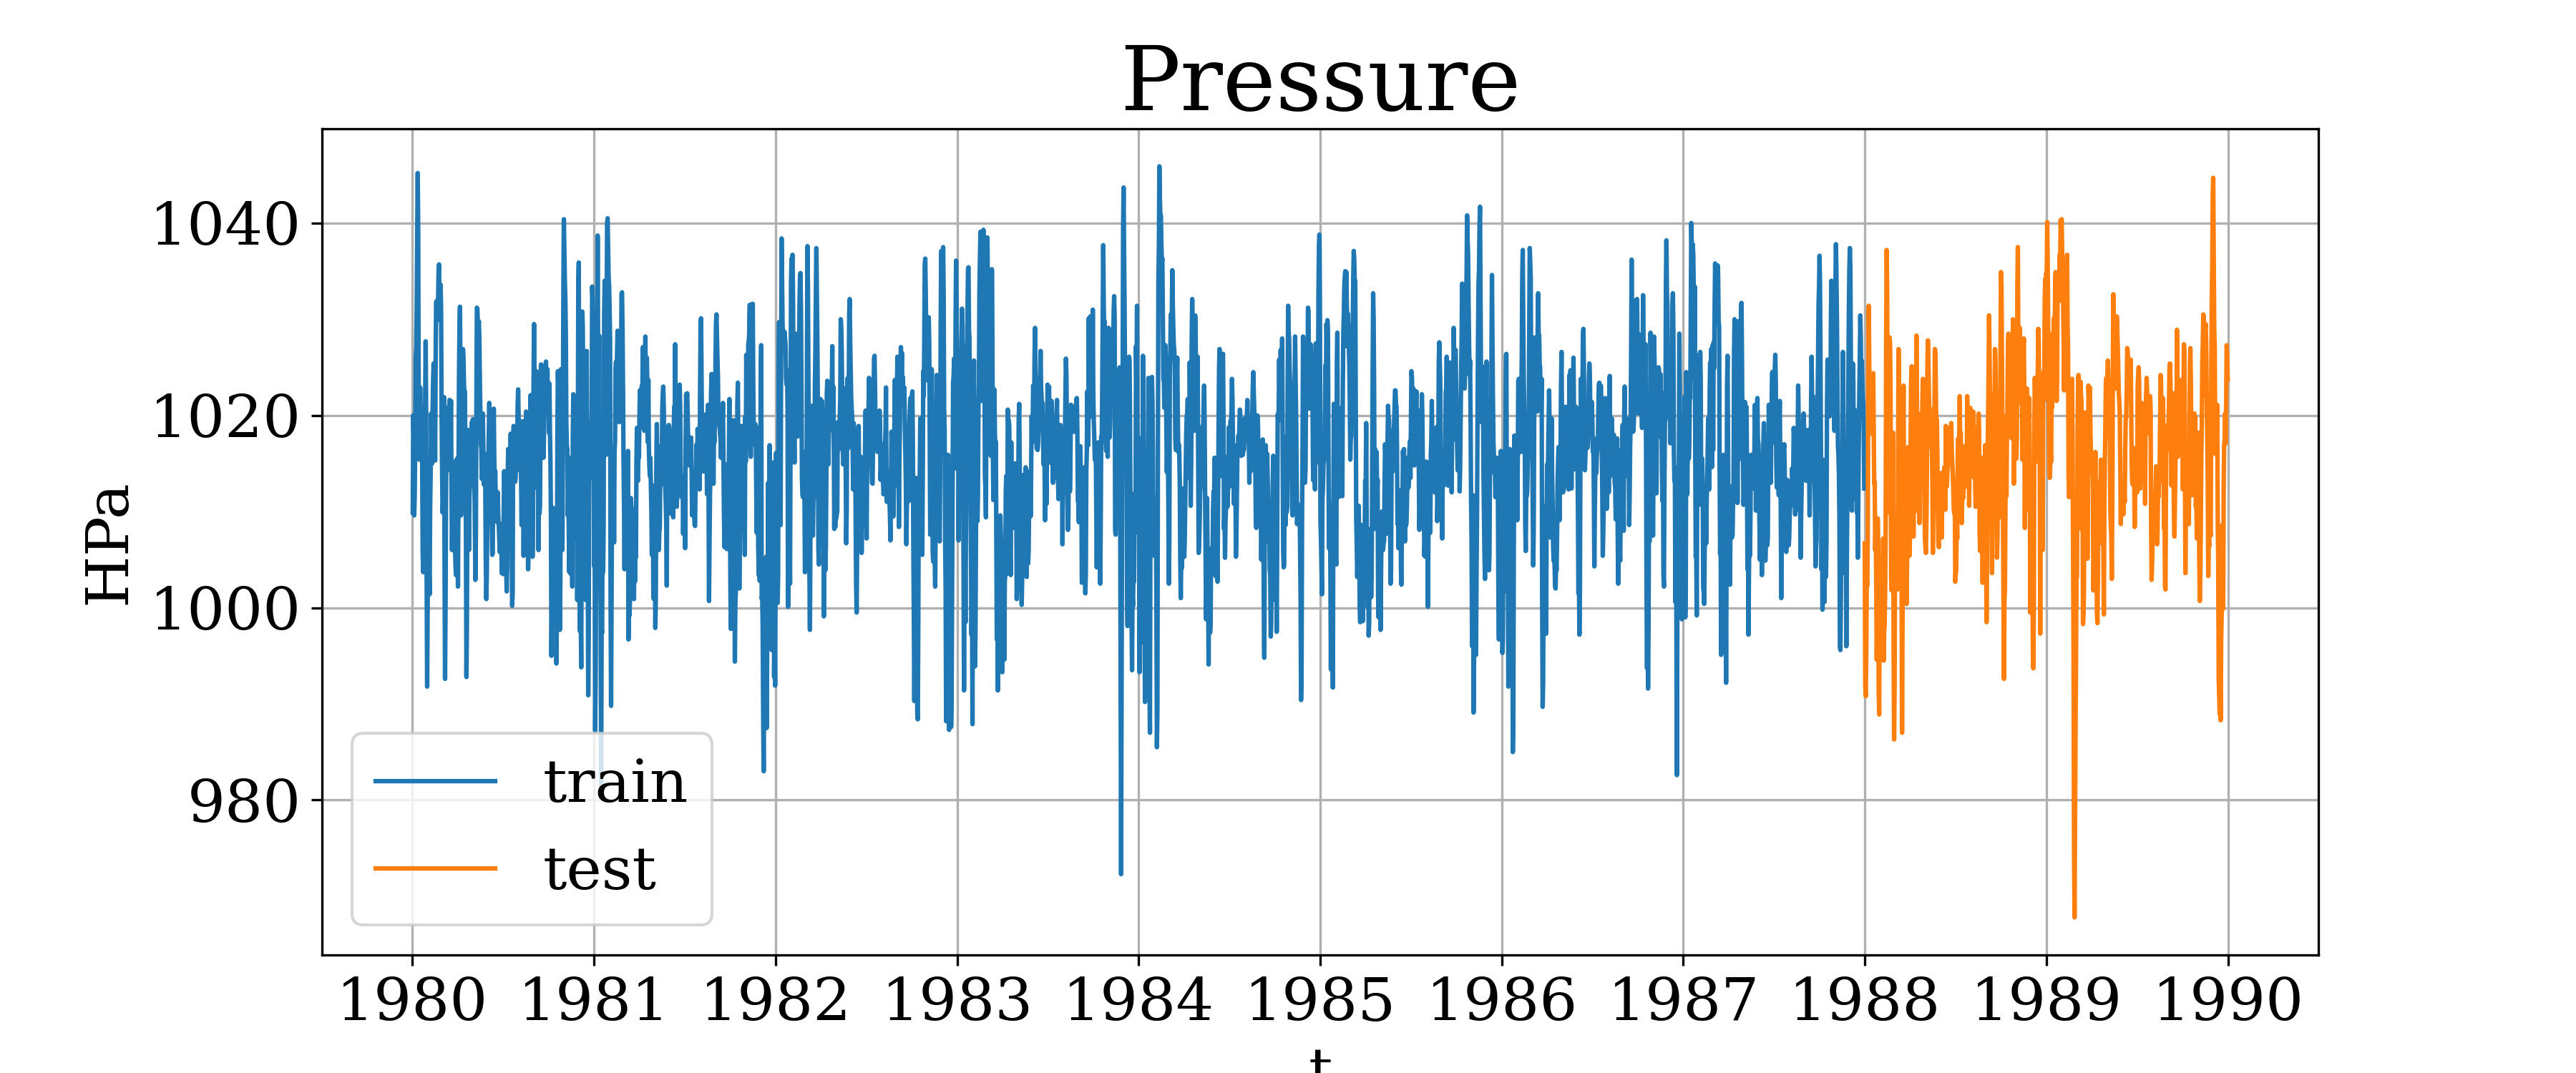
\includegraphics[width=0.48\textwidth, keepaspectratio]{../../figs/Pressure.png}
		\caption{Time series for temperature, precipitation and air pressure from meteostation in Berlin.}\label{fig:weather_data}
	\end{figure}
	
	Let's describe peculiarities of tSSA application. Firstly, tensor rank computation is NP-hard~\cite{HASTAD1990644}, so its number will be explicitly indicated whenever needed. Secondly, the used algorithm for CPD is ALS~\cite{kolda_tensors} and it has an approximation error. Thanks for that trajectory matrices' decomposition (\ref{eq:tSSA_decomp}) is not exact. This relative errors will be specified below. Thirdly, ILS problem (\ref{eq:decomp_search_final}) must be solved to find series decomposition. But matrix involved in it has a large row dimension. To boost computation we will cut it to several hundreds which is still much bigger then the size of sought parameter's vector. The used solver is SCIP~\cite{BolusaniEtal2024ZR}.

	Finally, let's fix a value $ L $ unified for all models. It is generally responsible for the size of series' history on which methods can be conditioned. For tSSA and mSSA it was described in the beginning of the section \ref{sec:problem_statement}. For RNN it is the length of encoder. For VAR it is the maximum lag number. We set $ L = 500 $.
	
	\subsection*{Results and discussion}
	
	We begin with forecast results. First, relation between prediction metrics for tSSA and trajectory tensor's rank is depicted on the fig. \ref{fig:mse_mape_electr} and \ref{fig:mse_mape_weather}. The minimum point and overall pattern are similar for MSE and MAPE. Furthermore, overtraining effect can be seen with especially sharp surge on the weather data. Nonetheless, CPD approximation error decease monotonously, fig. \ref{fig:cpd_errors}.
	
	\begin{figure}[h]
		\centering
		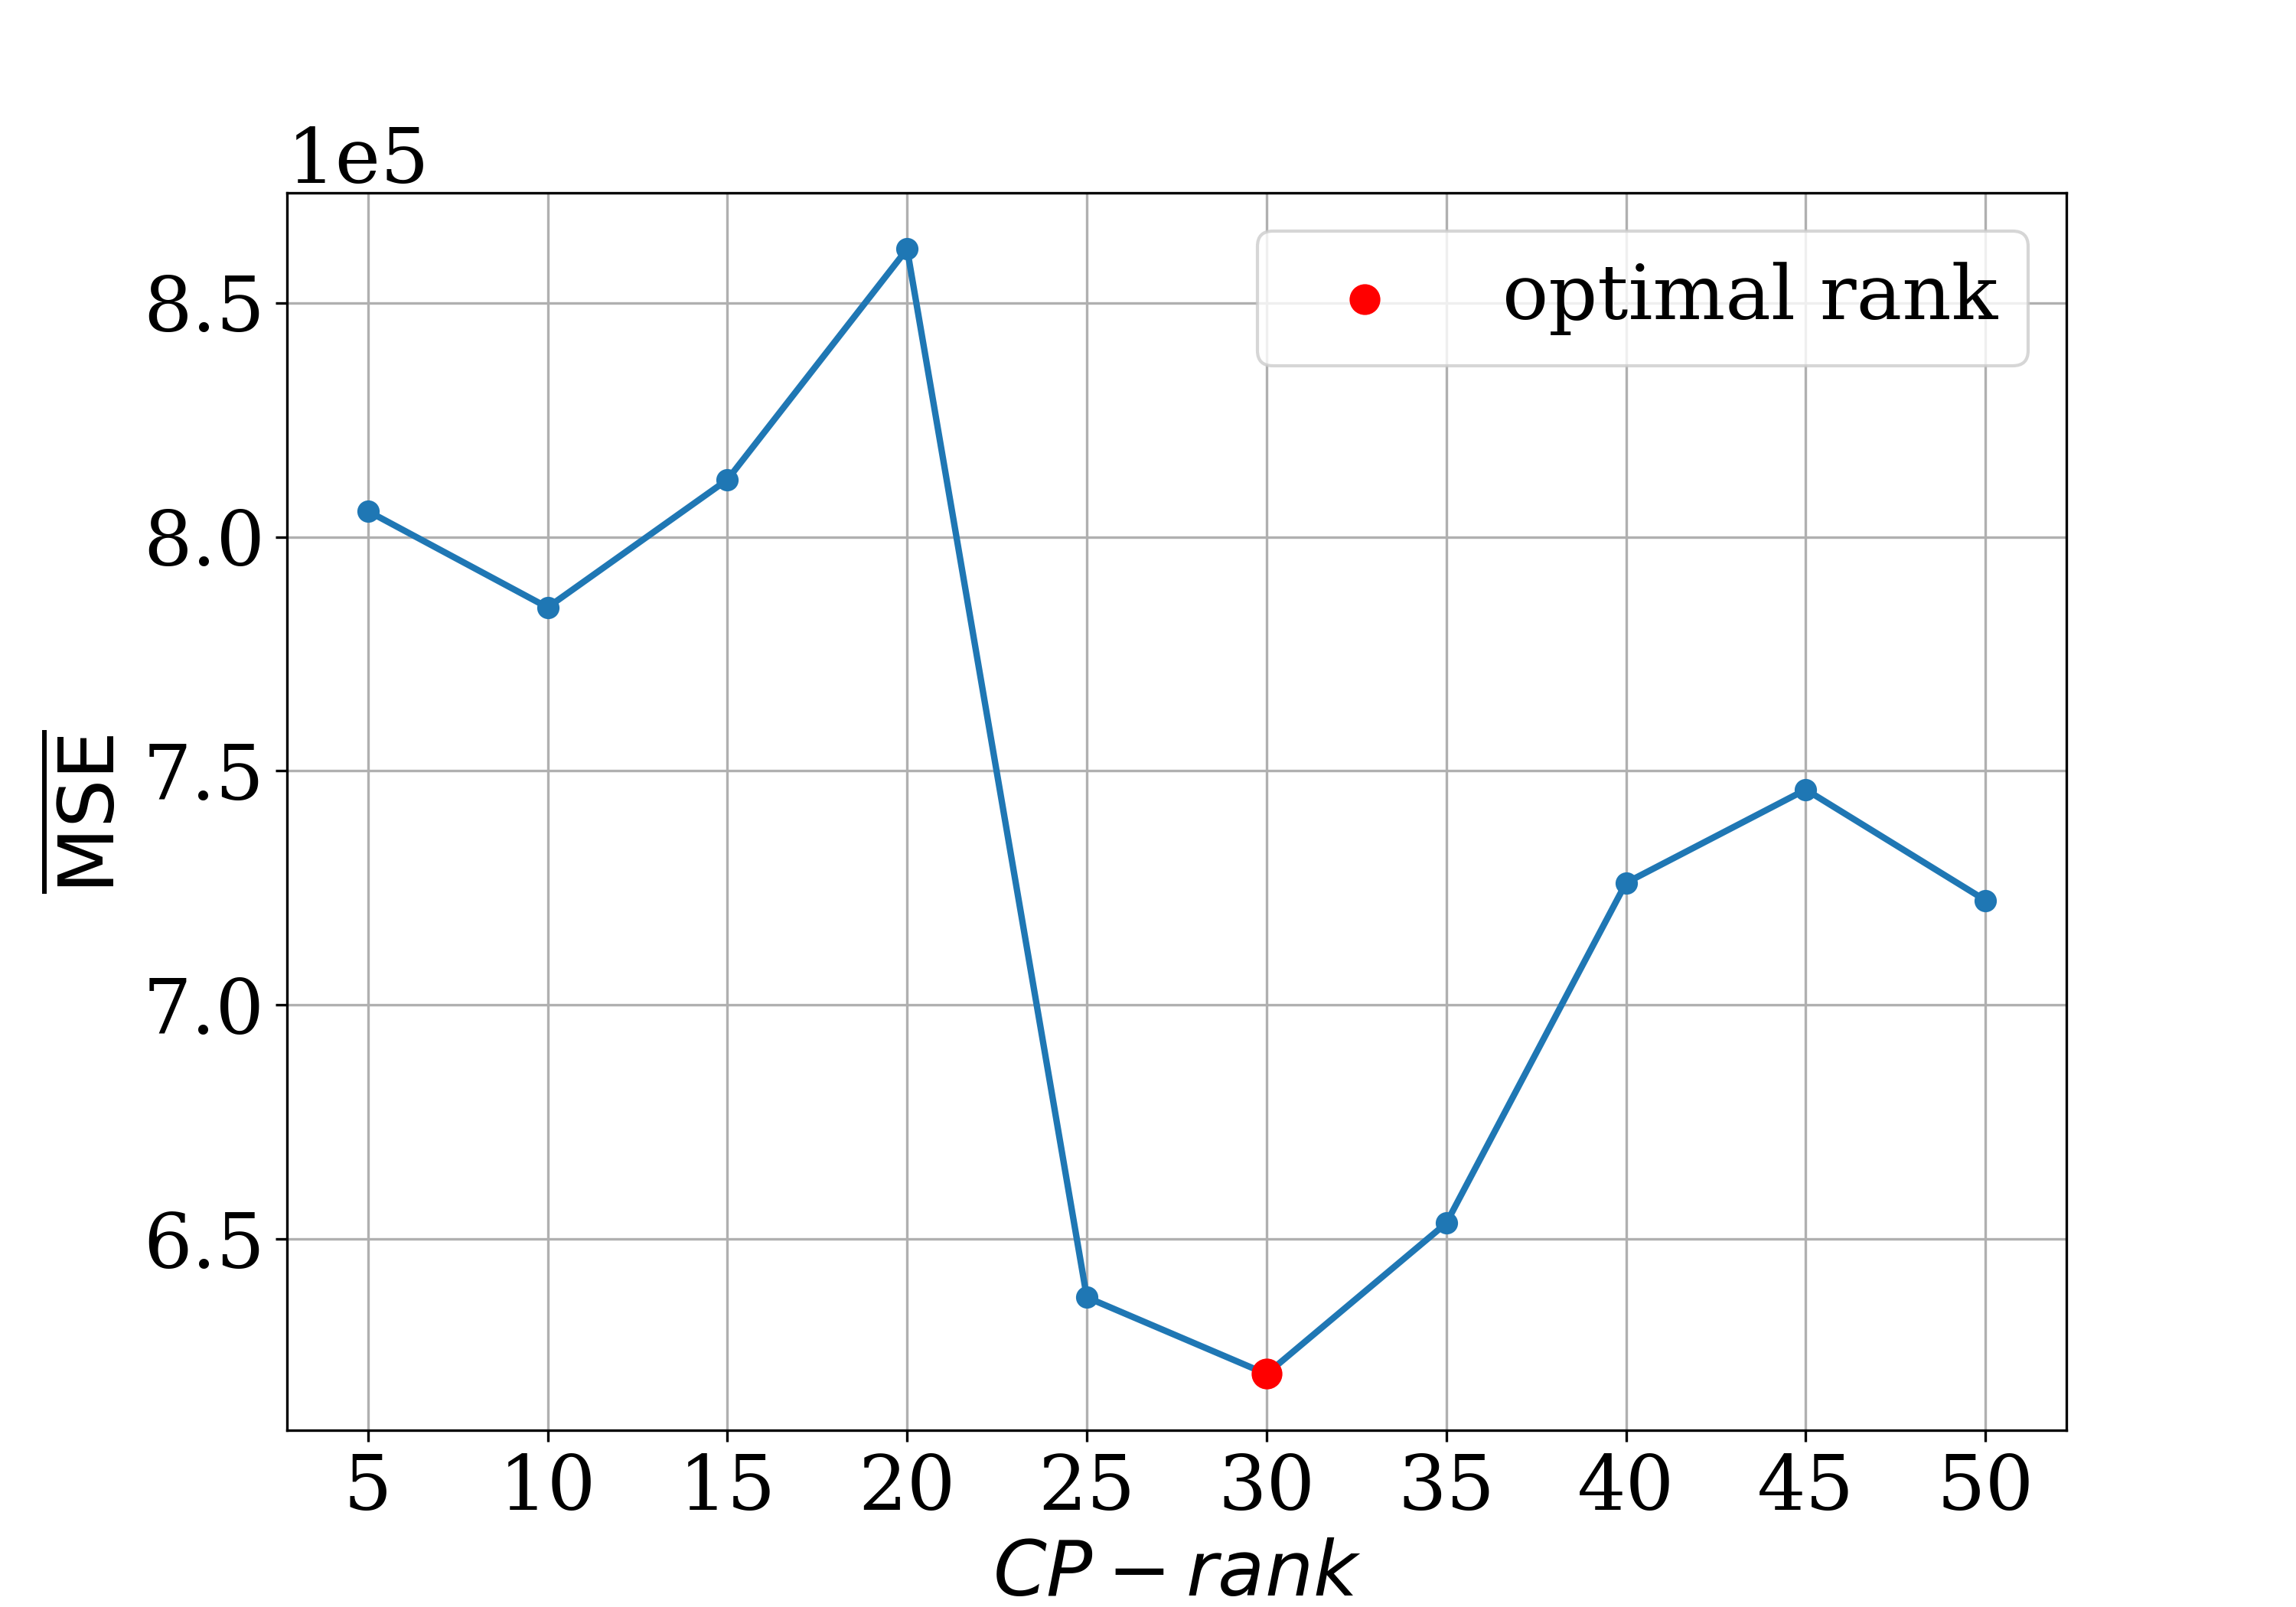
\includegraphics[width=0.48\textwidth, keepaspectratio]{../../experiments/electricity/tssa/figs/prediction/MSE_rank.png}
		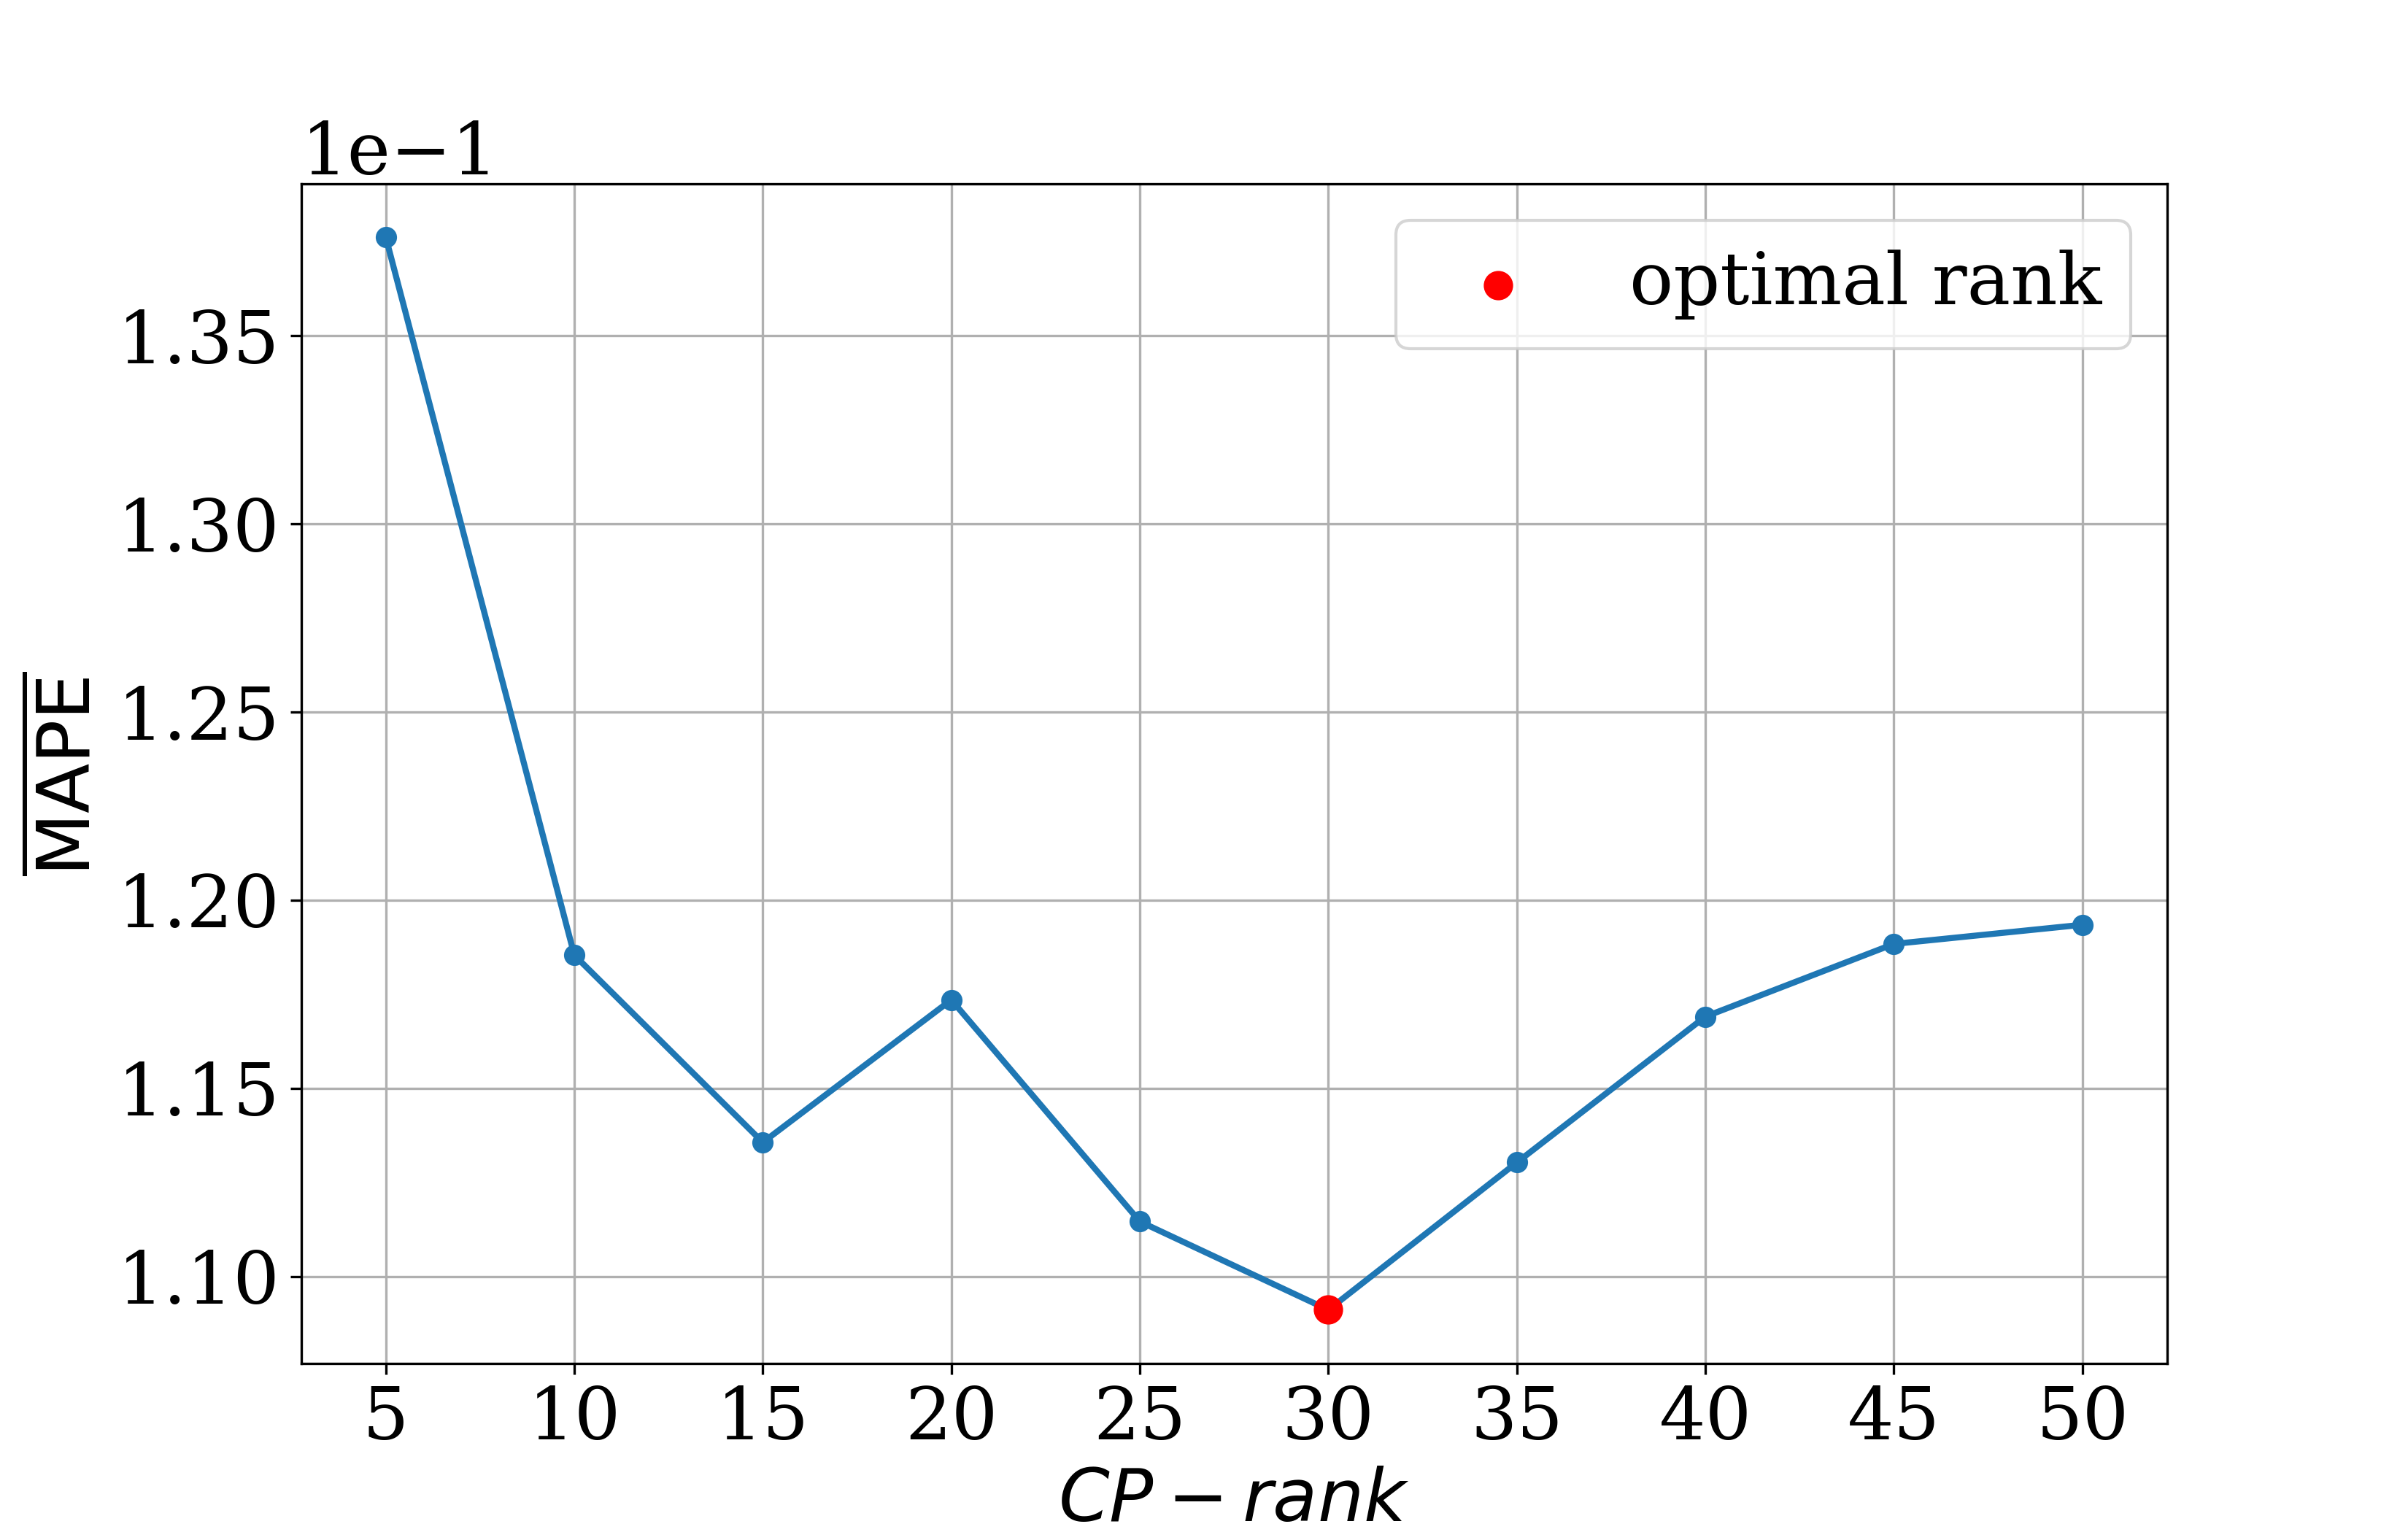
\includegraphics[width=0.48\textwidth, keepaspectratio]{../../experiments/electricity/tssa/figs/prediction/MAPE_rank.png}
		\caption{$ \overline{\text{MSE}} $ and $ \overline{\text{MAPE}} $ metrics for tSSA forecast depending on CPD rank. Optimal point is marked with red. Electricity data.}\label{fig:mse_mape_electr}
	\end{figure}
	
	\begin{figure}[h]
		\centering
		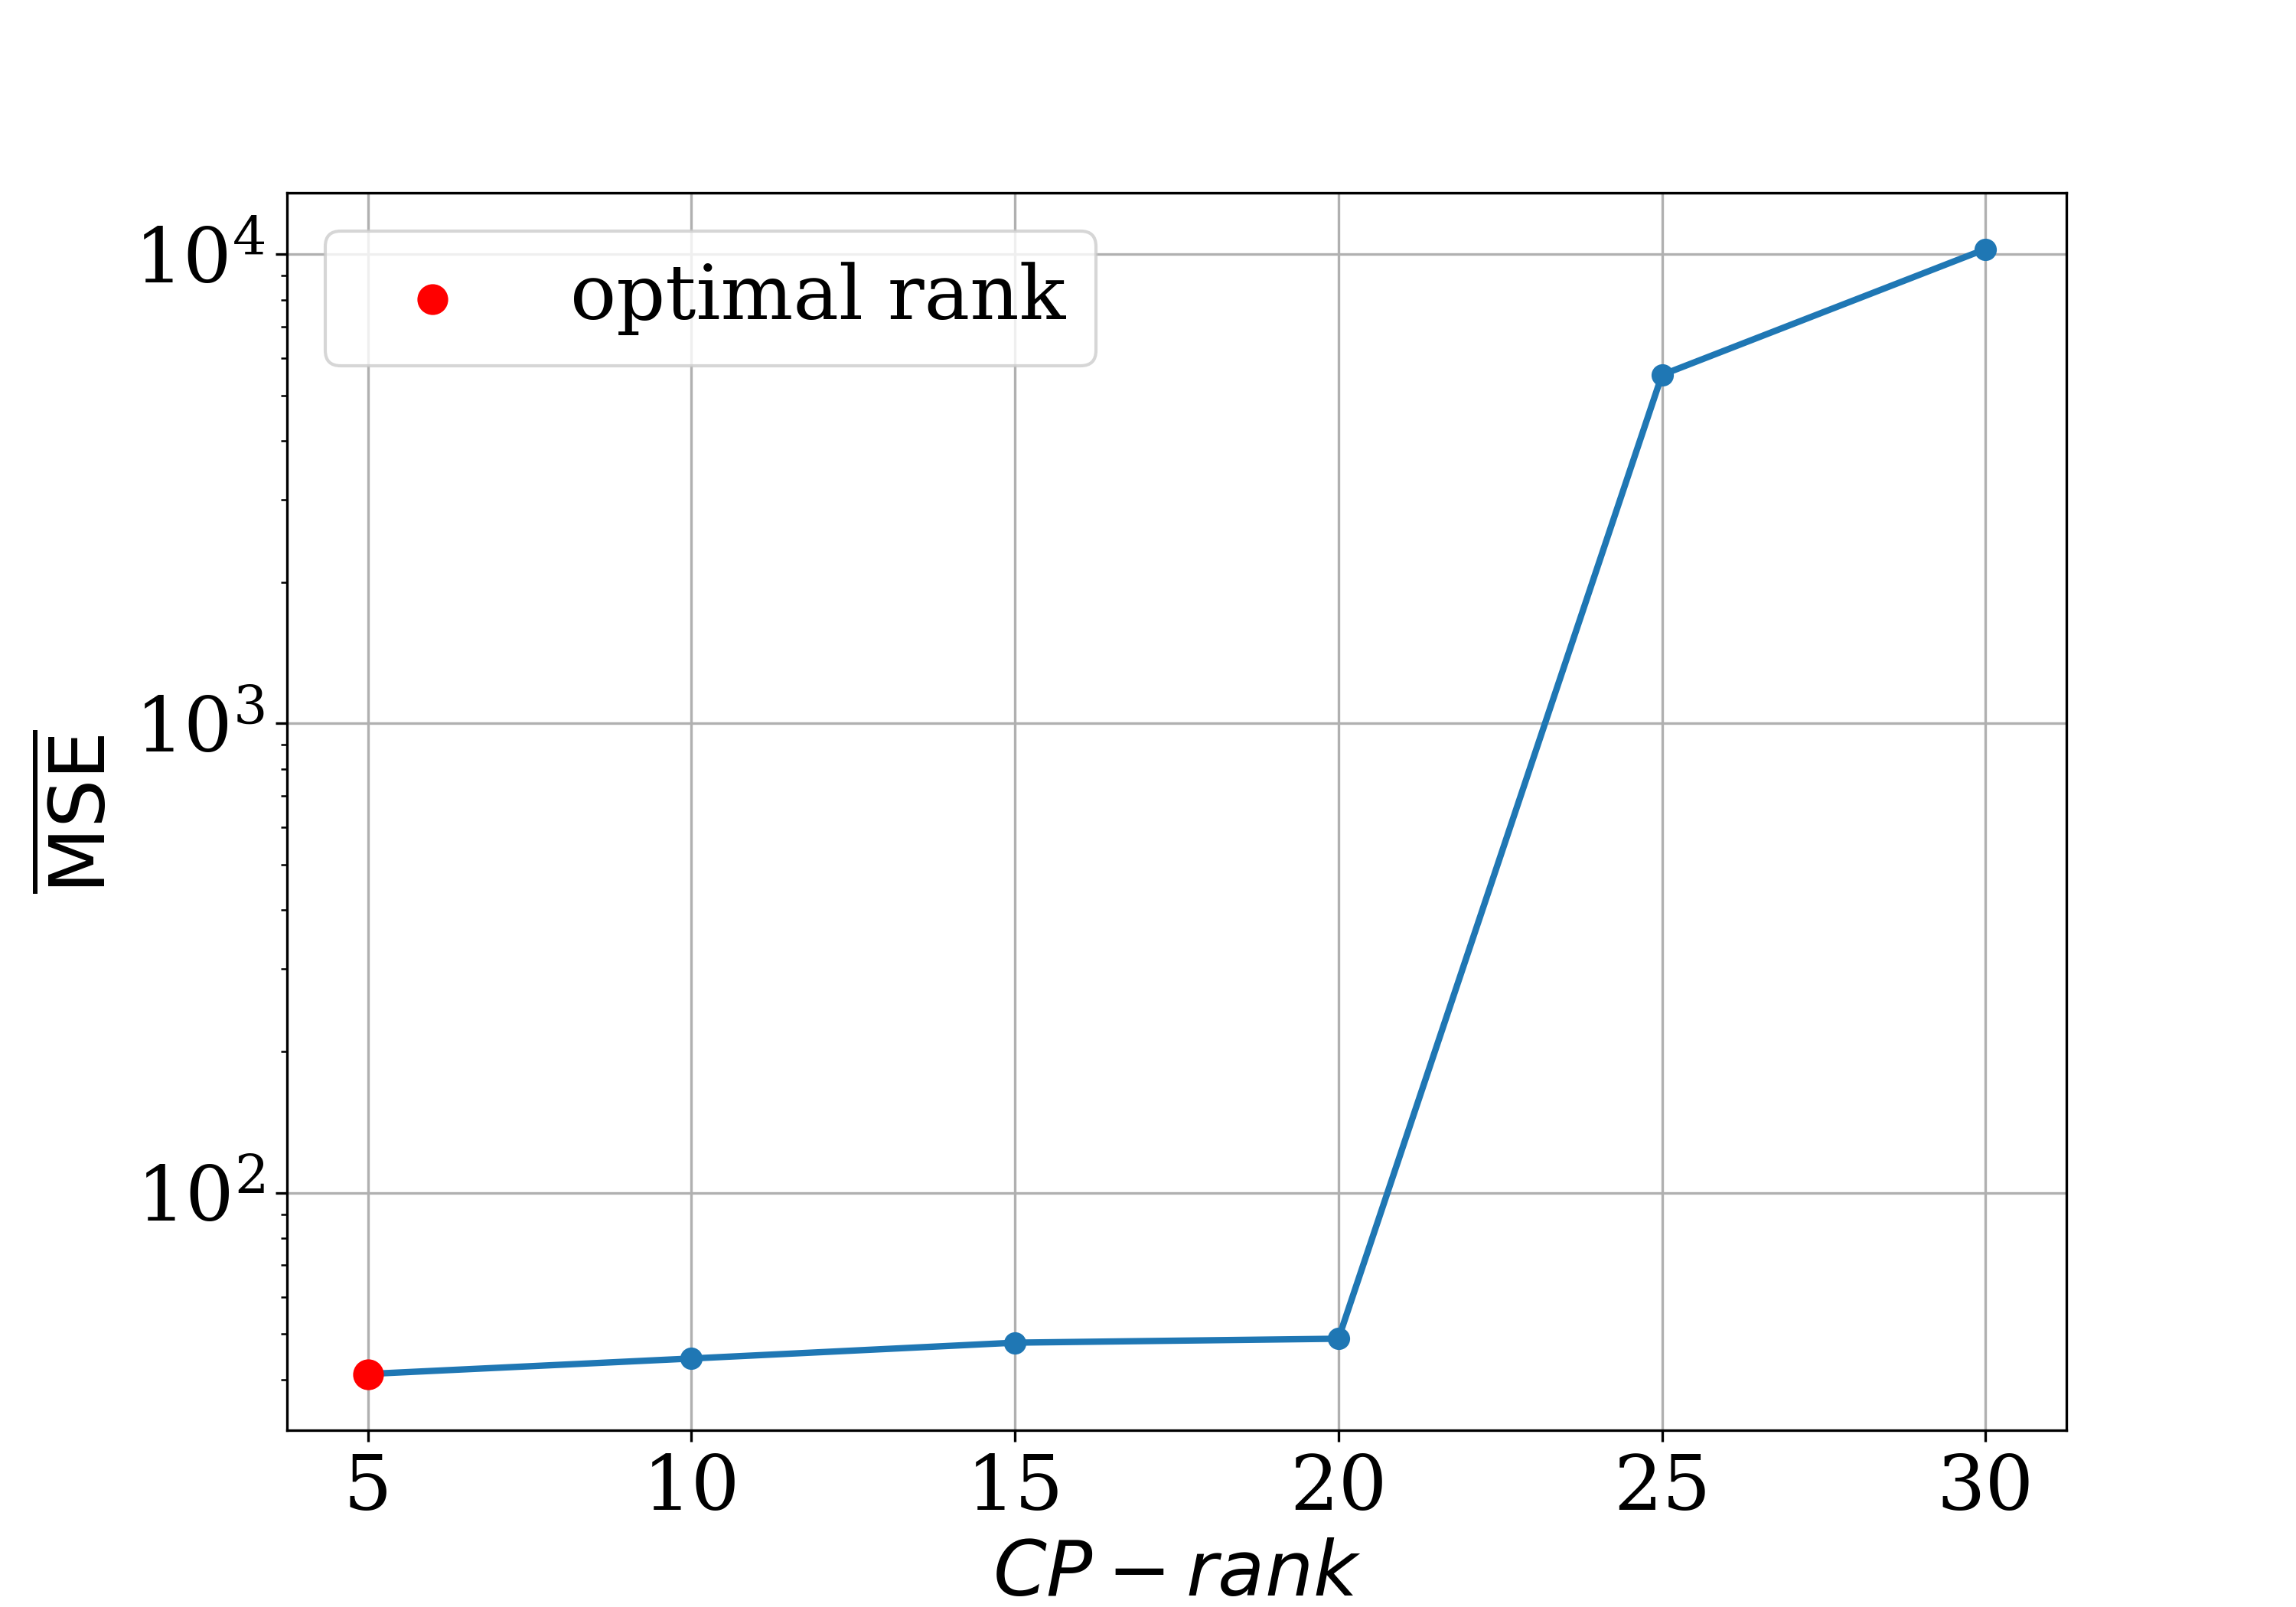
\includegraphics[width=0.48\textwidth, keepaspectratio]{../../experiments/weather/tssa/figs/prediction/MSE_rank.png}
		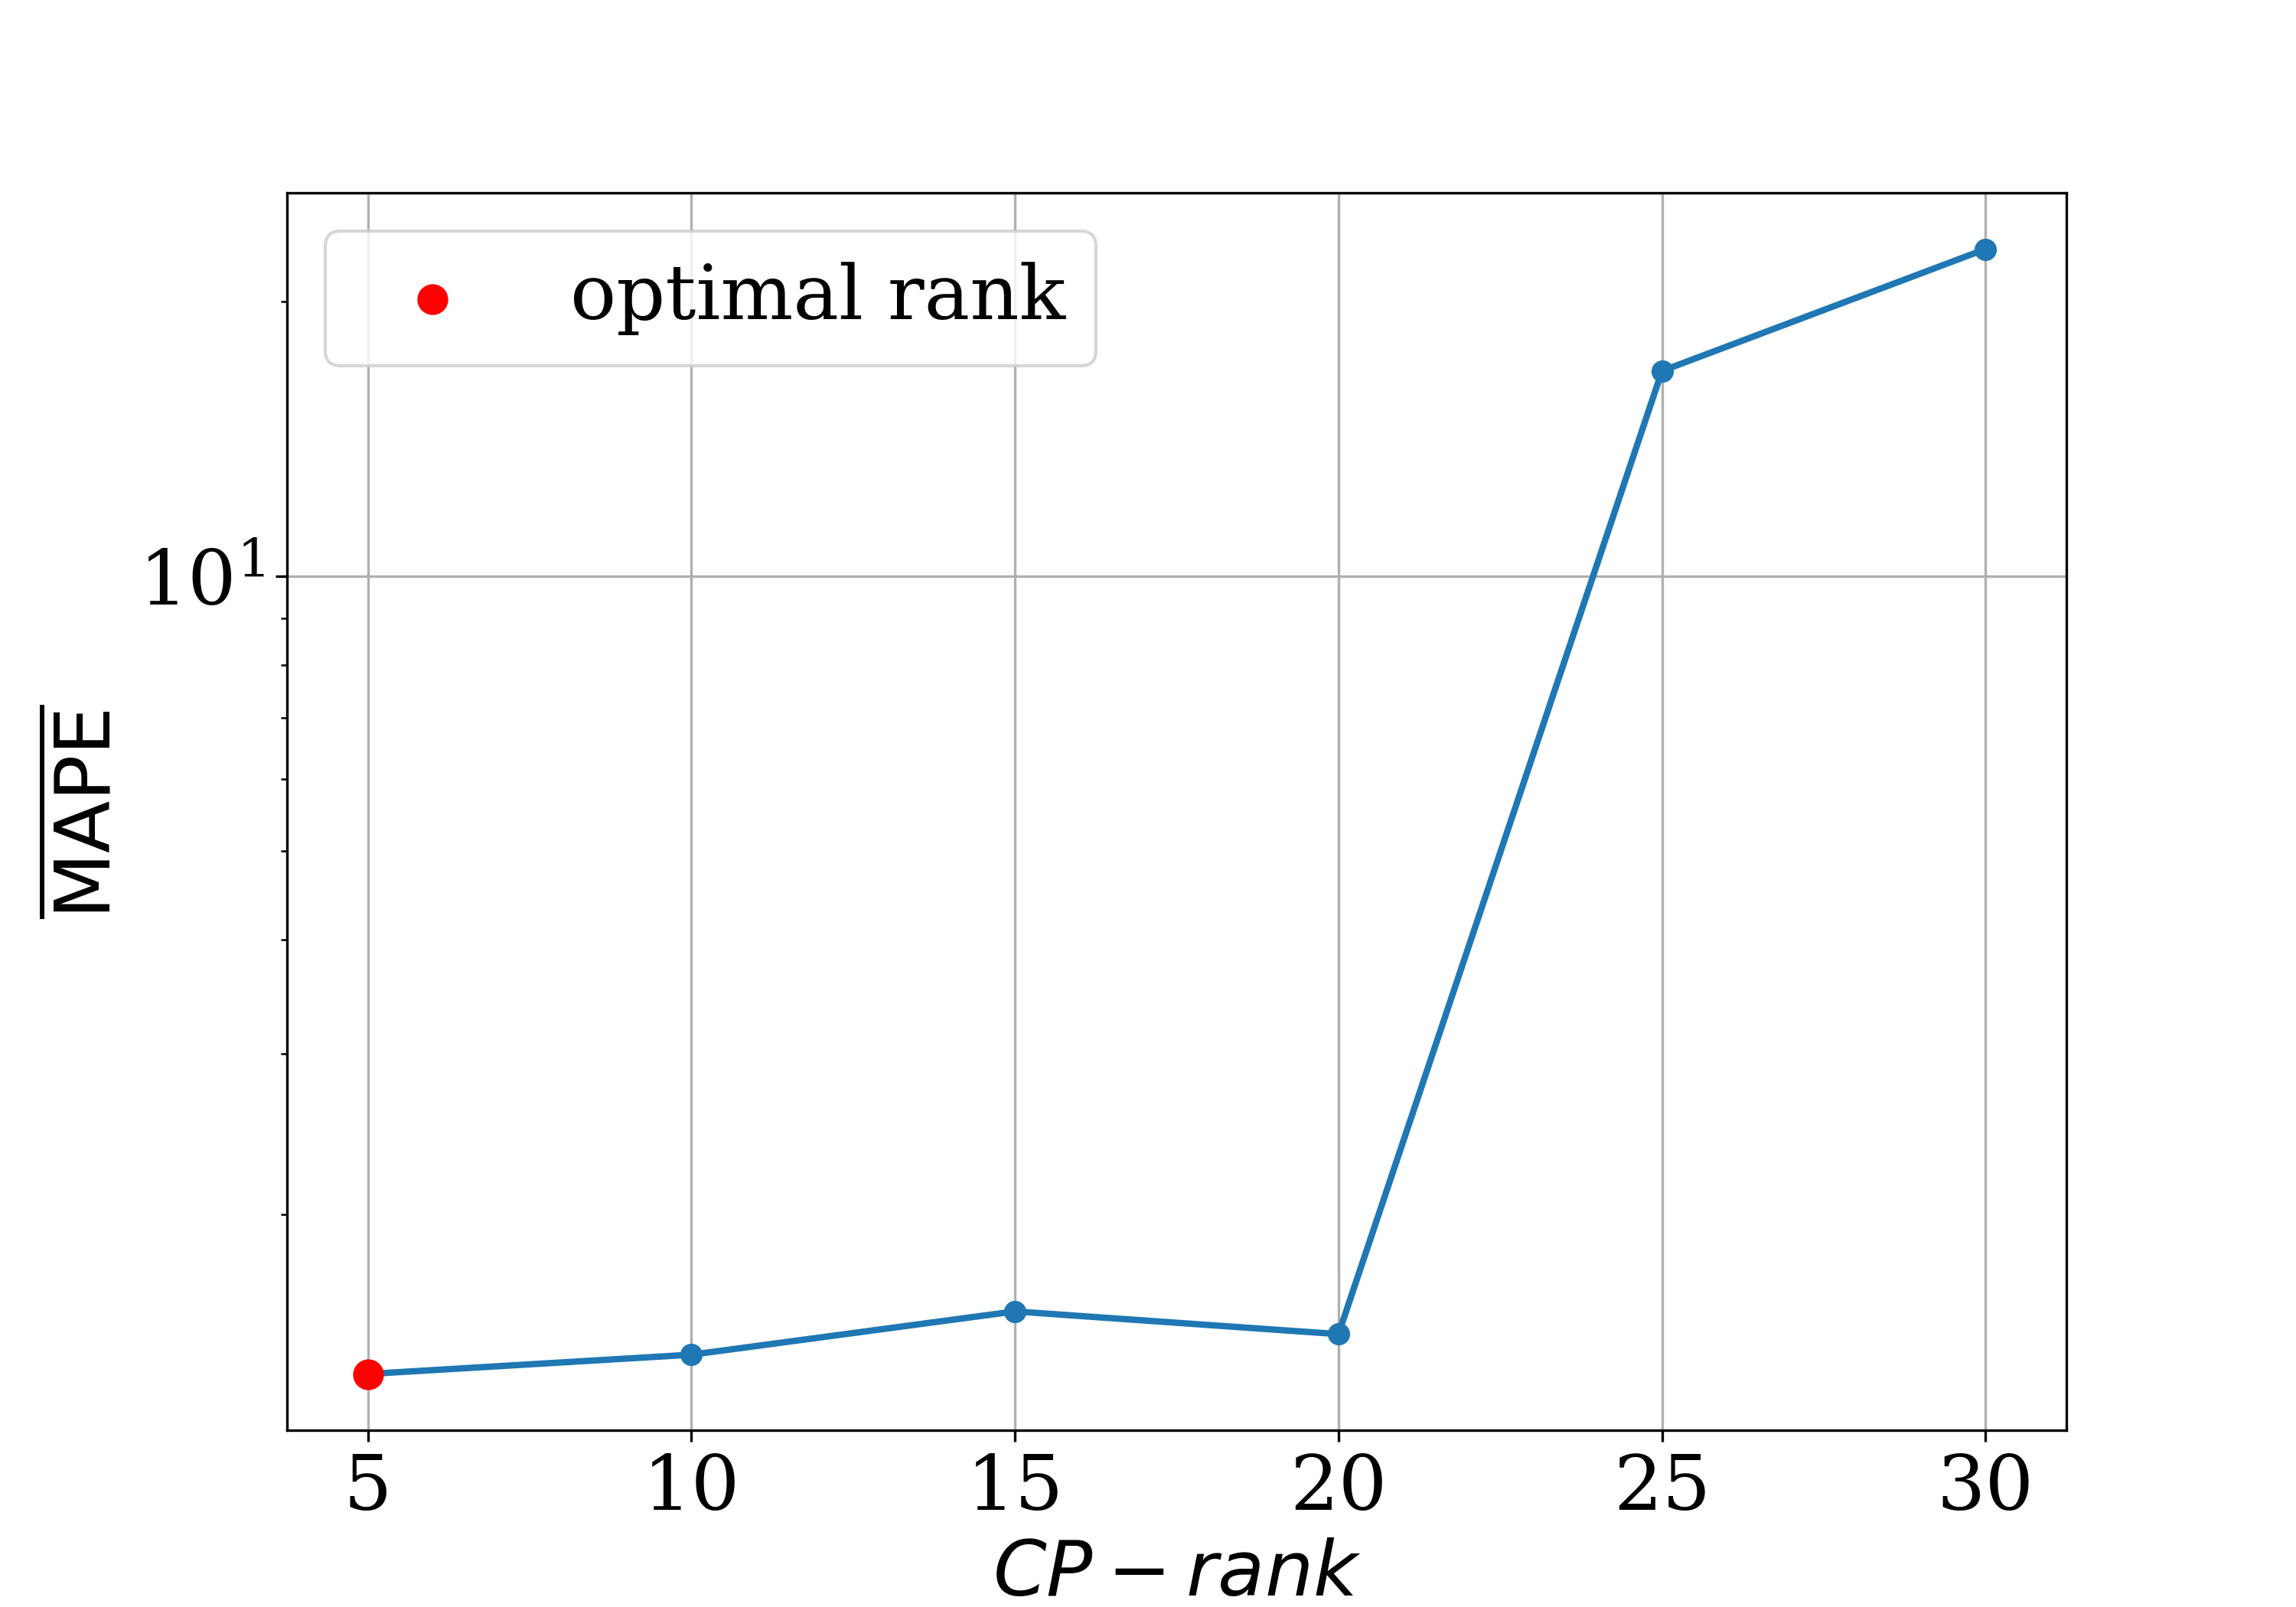
\includegraphics[width=0.48\textwidth, keepaspectratio]{../../experiments/weather/tssa/figs/prediction/MAPE_rank.png}
		\caption{$ \overline{\text{MSE}} $ and $ \overline{\text{MAPE}} $ metrics for tSSA forecast depending on CPD rank. Optimal point is marked with red. Weather data.}\label{fig:mse_mape_weather}
	\end{figure}
	
	\begin{figure}[h]
		\centering
		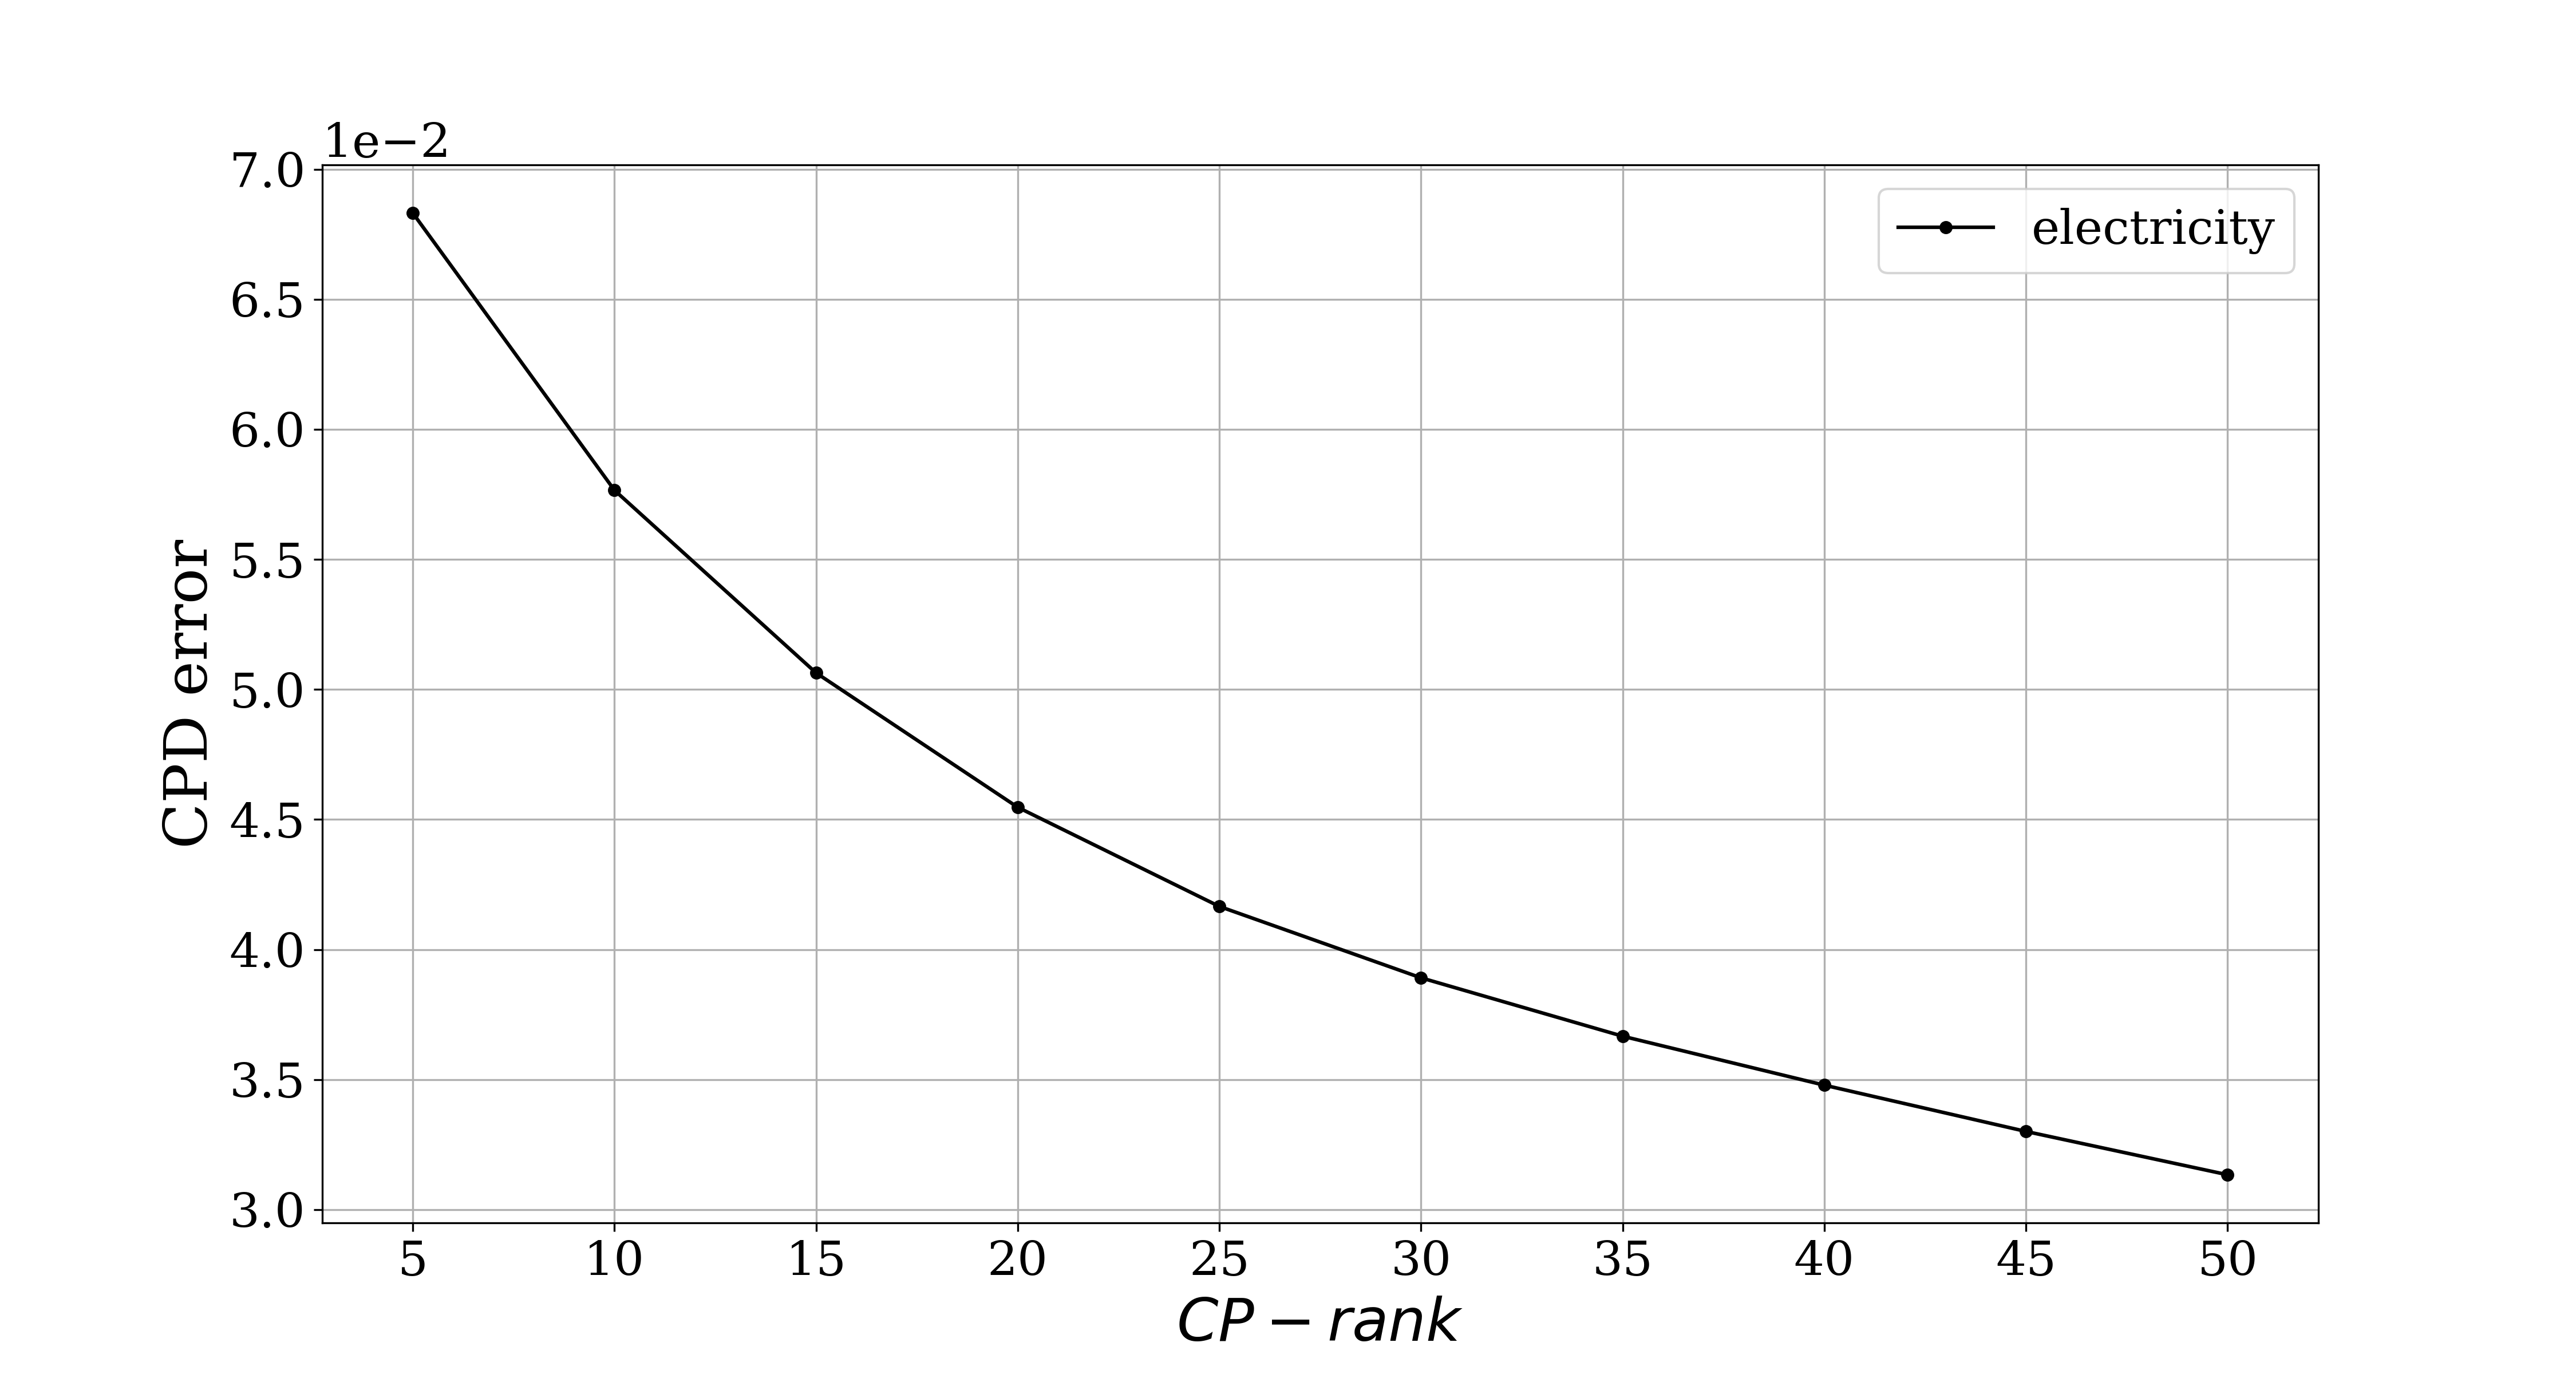
\includegraphics[width=0.48\textwidth, keepaspectratio]{../../experiments/electricity/tssa/figs/CPD_error.png}
		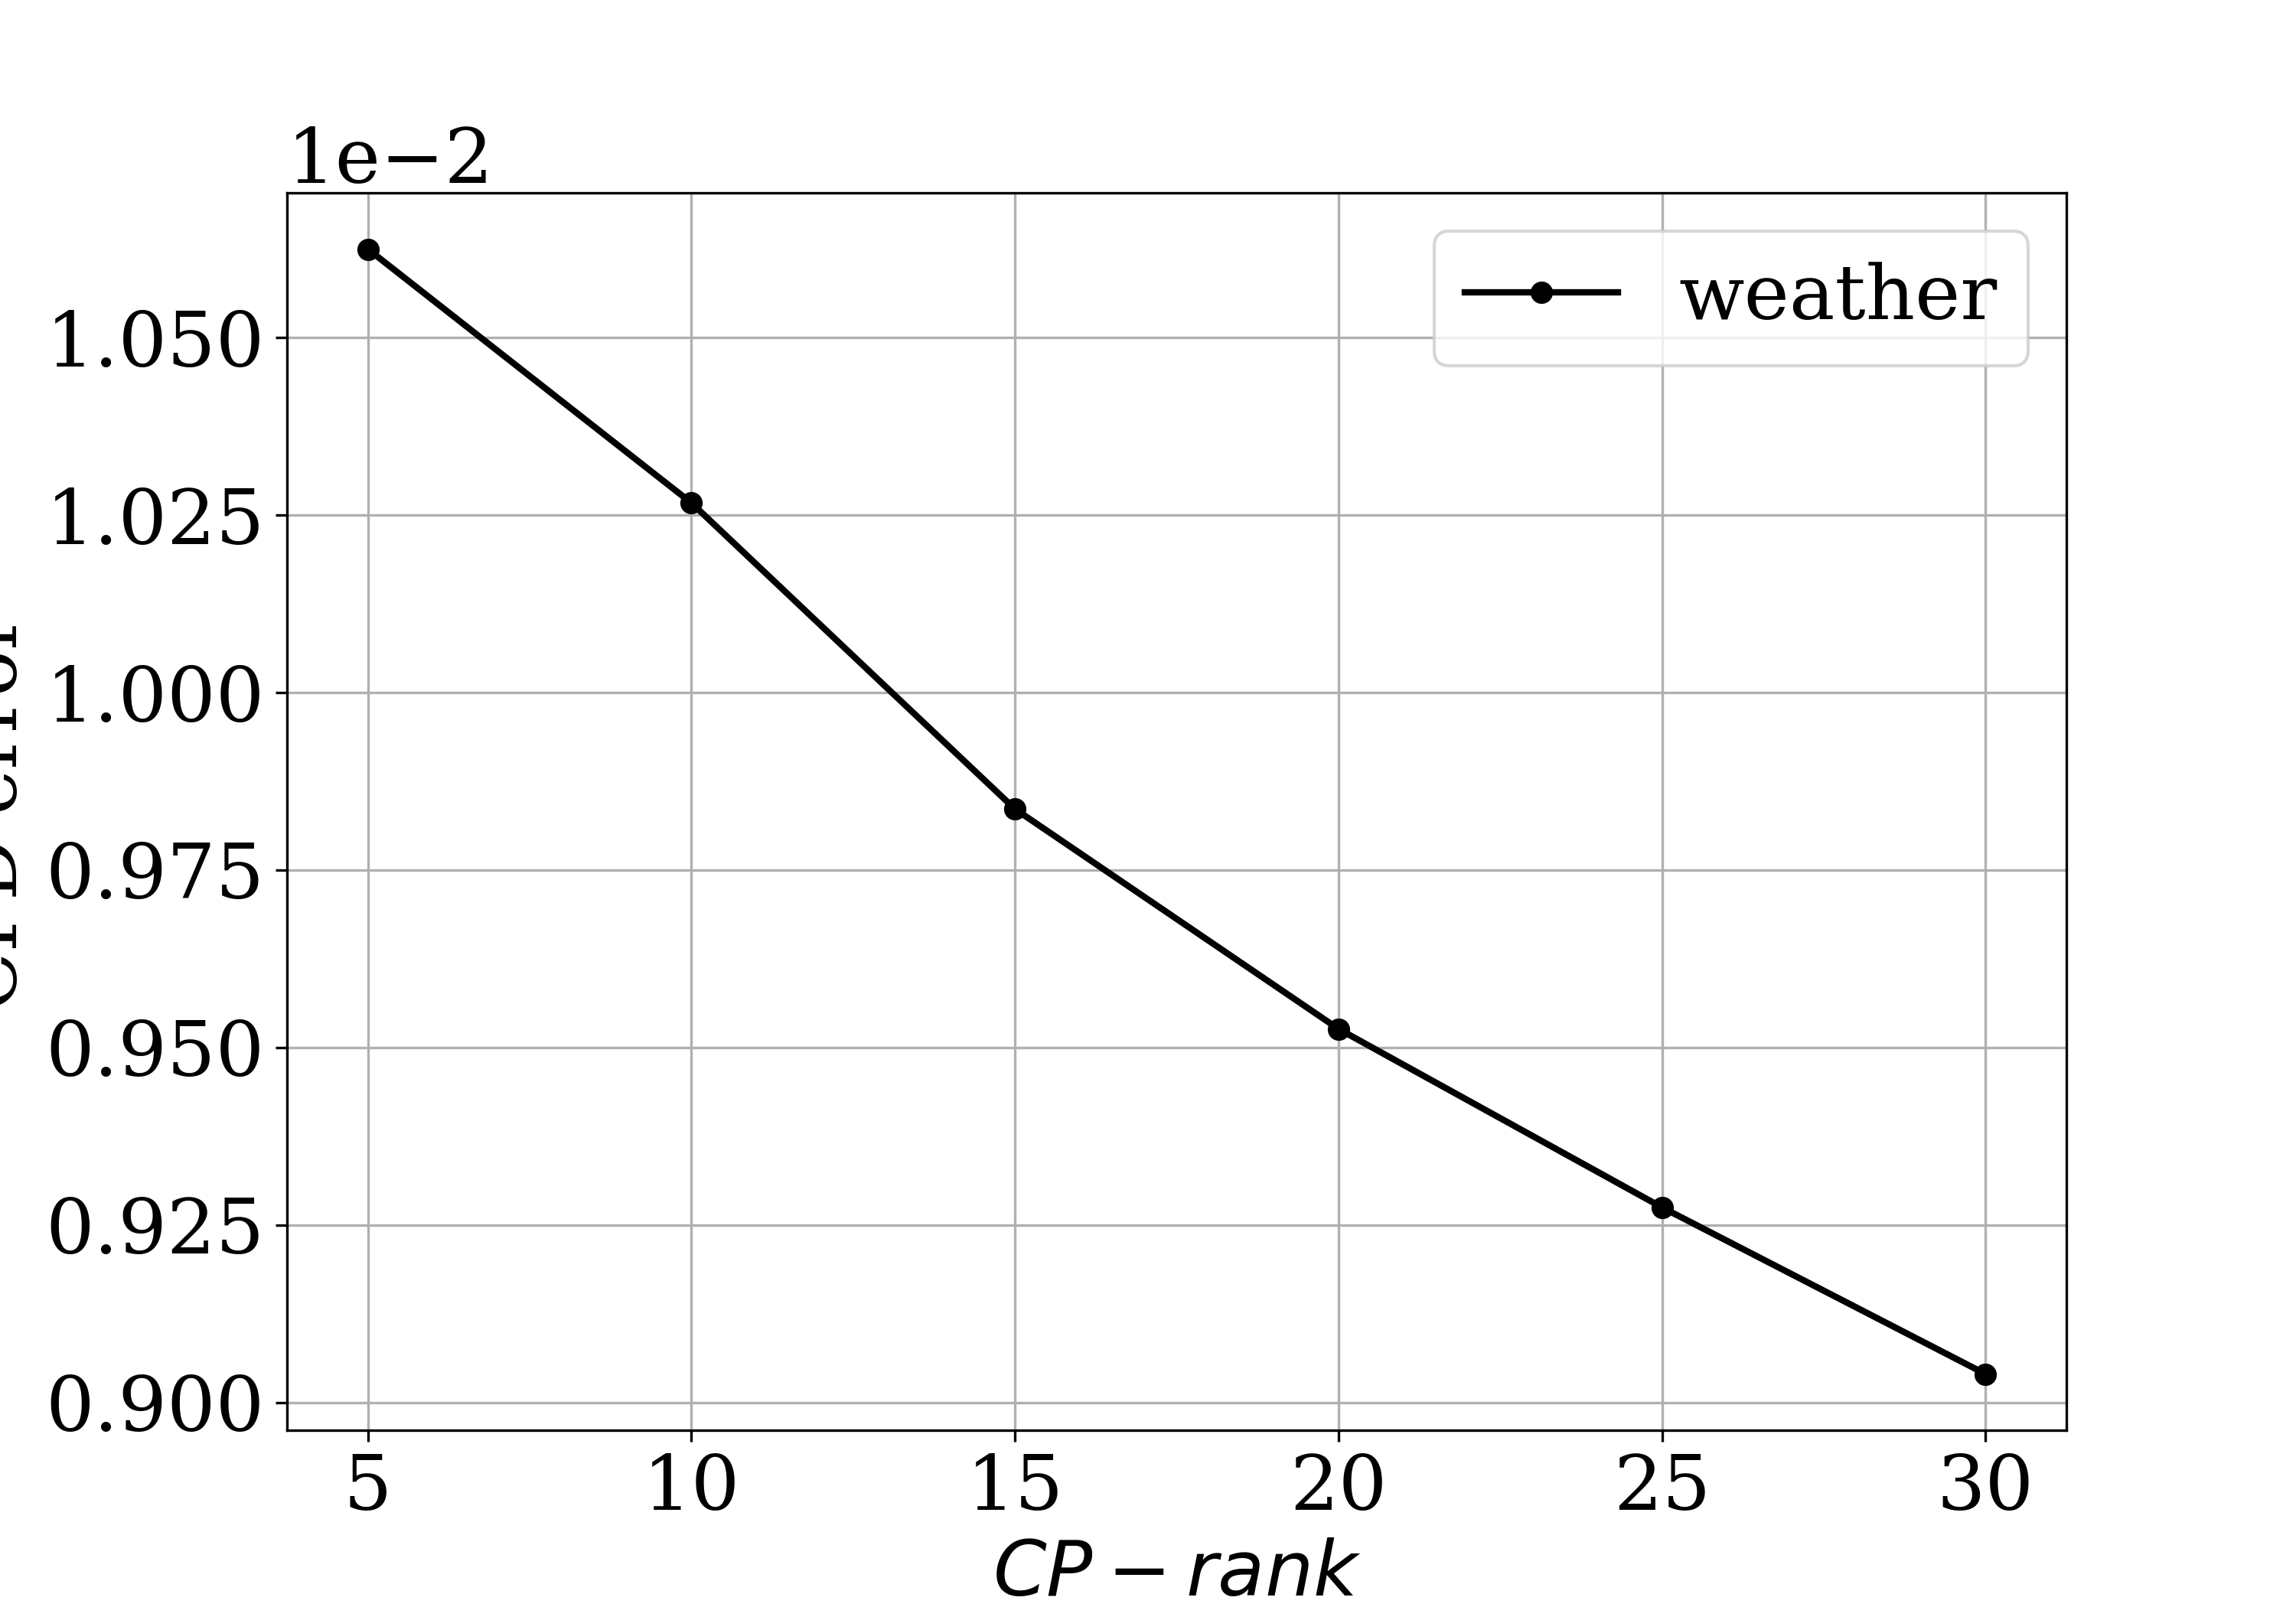
\includegraphics[width=0.48\textwidth, keepaspectratio]{../../experiments/weather/tssa/figs/CPD_error.png}
		\caption{Relative CPD approximation errors depending on CPD rank. Left is for electricity, right is for weather.}\label{fig:cpd_errors}
	\end{figure}
	
	The best tSSA forecast is shown on fig. \ref{fig:tssa_electr_pred} and \ref{fig:tssa_weather_pred}. For electricity CPD rank is rather high and so the order of autoregression forecast model (see \hyperref[sec:tssa_forecast]{Forecasting}). It allows for the complex prediction. On the other hand, for the weather high rank led to unstable and unbound forecast, but with the small rank one has few degrees of freedom. Consequently, we can only obtain some mean values for the future.
	
	The final forecast metrics for all models are in tab. \ref{tab:pred_res_electr} and \ref{tab:pred_res_weather}. Our method gave the best output. Close performance was shown by mSSA. The VAR model appeared unstable for the chosen prediction horizon and RNN could only learn the constant function from data.
	
	\def\arraystretch{1.1}
	\begin{table}[h]
		\centering
		\caption{Prediction quality of models for electricity data}\label{tab:pred_res_electr}
		\begin{tabular}{|c|c|c|c|c|}
			\hline
			& \textit{tSSA}  & \textit{mSSA} & \textit{VAR} & \textit{RNN} \\ \hline
			$ \overline{\text{MSE}}_{\text{Producution}} $, $10^6$ & 1.24           & 1.51          & 7.81         & 2.70         \\ \hline
			$ \overline{\text{MSE}}_{\text{Price}} $, $10^3$      & 0.88           & 1.03          & 4.85         & 30.0         \\ \hline
			$ \overline{\text{MSE}} $, $10^6$             & \textbf{0.62}  & 0.75          & 3.91         & 135.00       \\ \hline
			$ \overline{\text{MAPE}}_{\text{Producution}} $        & 0.054          & 0.060         & 0.137        & 0.999        \\ \hline
			$ \overline{\text{MAPE}}_{\text{Price}} $             & 0.164          & 0.170         & 0.360        & 1.004        \\ \hline
			$ \overline{\text{MAPE}} $                    & \textbf{0.109} & 0.115         & 0.249        & 1.002        \\ \hline
		\end{tabular}
	\end{table}
	
	\def\arraystretch{1.1}
	\begin{table}[h]
		\centering
		\caption{Prediction quality of models for weather data}\label{tab:pred_res_weather}
		\begin{tabular}{|c|c|c|c|c|}
			\hline
			& \textit{tSSA}                & \textit{mSSA} & \textit{VAR} & \textit{RNN} \\ \hline
			$ \overline{\text{MSE}}_{\text{Temp}} $  & 14.16                        & 20.12         & 40.67        & -            \\ \hline
			$ \overline{\text{MSE}}_{\text{Prec}} $  & 11.02                        & 11.23         & 22.84        & -            \\ \hline
			$ \overline{\text{MSE}}_{\text{Pres}} $  & 98.02                        & 101.23        & 156.75       & -            \\ \hline
			$ \overline{\text{MSE}} $        & \textbf{41.067}              & 44.193        & 73.420       & -            \\ \hline
			$ \overline{\text{MAPE}}_{\text{Temp}} $ & 0.850 & 0.626         & 0.468        & -            \\ \hline
			$ \overline{\text{MAPE}}_{\text{Prec}} $ & 3.151 & 2.834         & 4.637        & -            \\ \hline
			$ \overline{\text{MAPE}}_{\text{Pres}} $ & 0.007 & 1.254         & 3.983        & -            \\ \hline
			$ \overline{\text{MAPE}} $       & \textbf{1.336}               & 1.571         & 3.029        & -            \\ \hline
		\end{tabular}
	\end{table}
	
	Now we move to the decomposition. Fig. \ref{fig:decomp_rhe_rank} illustrates relation between quality metrics and CPD rank. In both cases $ \overline{\text{RHE}} $ rapidly reaches a minimum and then does not change or even increase. Recalling the same result for the forecast we can conclude that tSSA has the greatest generalization capacity for the small tensor ranks. At the same time, the rank is proportional to the signal subspace dimensionality (see section \ref{sec:problem_statement}). So this approves the major premise of our method --- small real dimension of the data.s
	
	One the fig. \ref{fig:electr_decomp_tssa}, \ref{fig:weather_decomp_tssa} one can see best tSSA's decomposition on two components. Due to rather long computation of ILS we do not make more. And it is not necessary to catch the notion of shared basis for observed signals in a set. For example, decomposition for electricity generation and its price are almost identical up to the bias and scale. The same situation is for temperature and precipitation from the weather data, but air pressure got its own components. Now, let's interpret obtained results. On the fig. \ref{fig:weather_decomp_tssa} method extracted two periodical parts for each signal with large and much smaller amplitudes. Some noise is present in each component. On the fig. \ref{fig:electr_decomp_tssa} we have two high-frequency harmonics with different amplitude and bias.	
	
	In comparison, we present mSSA's decomposition on five components,  fig. \ref{fig:electr_decomp_mssa} and \ref{fig:weather_decomp_mssa}. There is no need to solve heavy ILS problem or pick over CPD rank, but it is a manual procedure based on singular values analysis of some matrix~\cite{ecfb9dc578be43ae9ee8fc88b8ff9151}. Nonetheless, the gained  components are simpler and more diverse --- algorithm extracted several trends and harmonics. Moreover, mSSA has slight advantage in decomposition quality as described in tab. \ref{tab:decomp_electr_results}, \ref{tab:decomp_weather_results}. To conclude, the complexity of tSSA decomposition problem is the major stumbling block of our method which requires development of its own solutions and heuristics. For the record, mSSA has already had those~\cite{ecfb9dc578be43ae9ee8fc88b8ff9151}.
	
	\def\arraystretch{1.2}
	\begin{table}[h!]
		\centering
		\caption{Decomposition quality of models for electricity data}\label{tab:decomp_electr_results}
		\begin{tabular}{|c|c|c|}
			\hline
			& tSSA  & mSSA           \\ \hline
			$ \overline{\text{RHE}}_{\text{Producution}} $  & 0.507 & 0.308          \\ \hline
			$ \overline{\text{RHE}}_{\text{Price}} $      & 0.511 & 0.31           \\ \hline
			$ \overline{\text{RHE}} $             & 0.509 & \textbf{0.309} \\ \hline
		\end{tabular}
	\end{table}
	
	\def\arraystretch{1.2}
	\begin{table}[h!]
		\centering
		\caption{Decomposition quality of models for weather data}\label{tab:decomp_weather_results}
		\begin{tabular}{|c|c|c|}
			\hline
			& tSSA  & mSSA           \\ \hline
			$ \overline{\text{RHE}}_{\text{Temp}} $   & 0.512 & 0.467          \\ \hline
			$ \overline{\text{RHE}}_{\text{Prec}} $ & 0.508 & 0.538          \\ \hline
			$ \overline{\text{RHE}}_{\text{Pres}} $   & 0.542 & 0.502          \\ \hline
			$ \overline{\text{RHE}} $         & 0.521 & \textbf{0.502} \\ \hline
		\end{tabular}
	\end{table}	
	
	\section{Conclusion}
	
		Tensor method tSSA is devoted to prediction and decomposition of multidimensional time series with substantial interconnection between them. It is easy to use --- there are only two adjustable parameters which does not require heavy learning procedures. Besides, the theory behind is based on the general framework of dynamical systems and demands only low-dimensional representation of data. When applied to real sets of signals, these assumptions were confirmed as well as the neural and statistical models were outperformed by our approach. Nonetheless, a bottleneck was discovered which is NP-hardness of optimal series decomposition. Resolving this problem or finding another way to build signal's components are the major ways for further improvement.
		
		\begin{figure}[h]
			\centering
			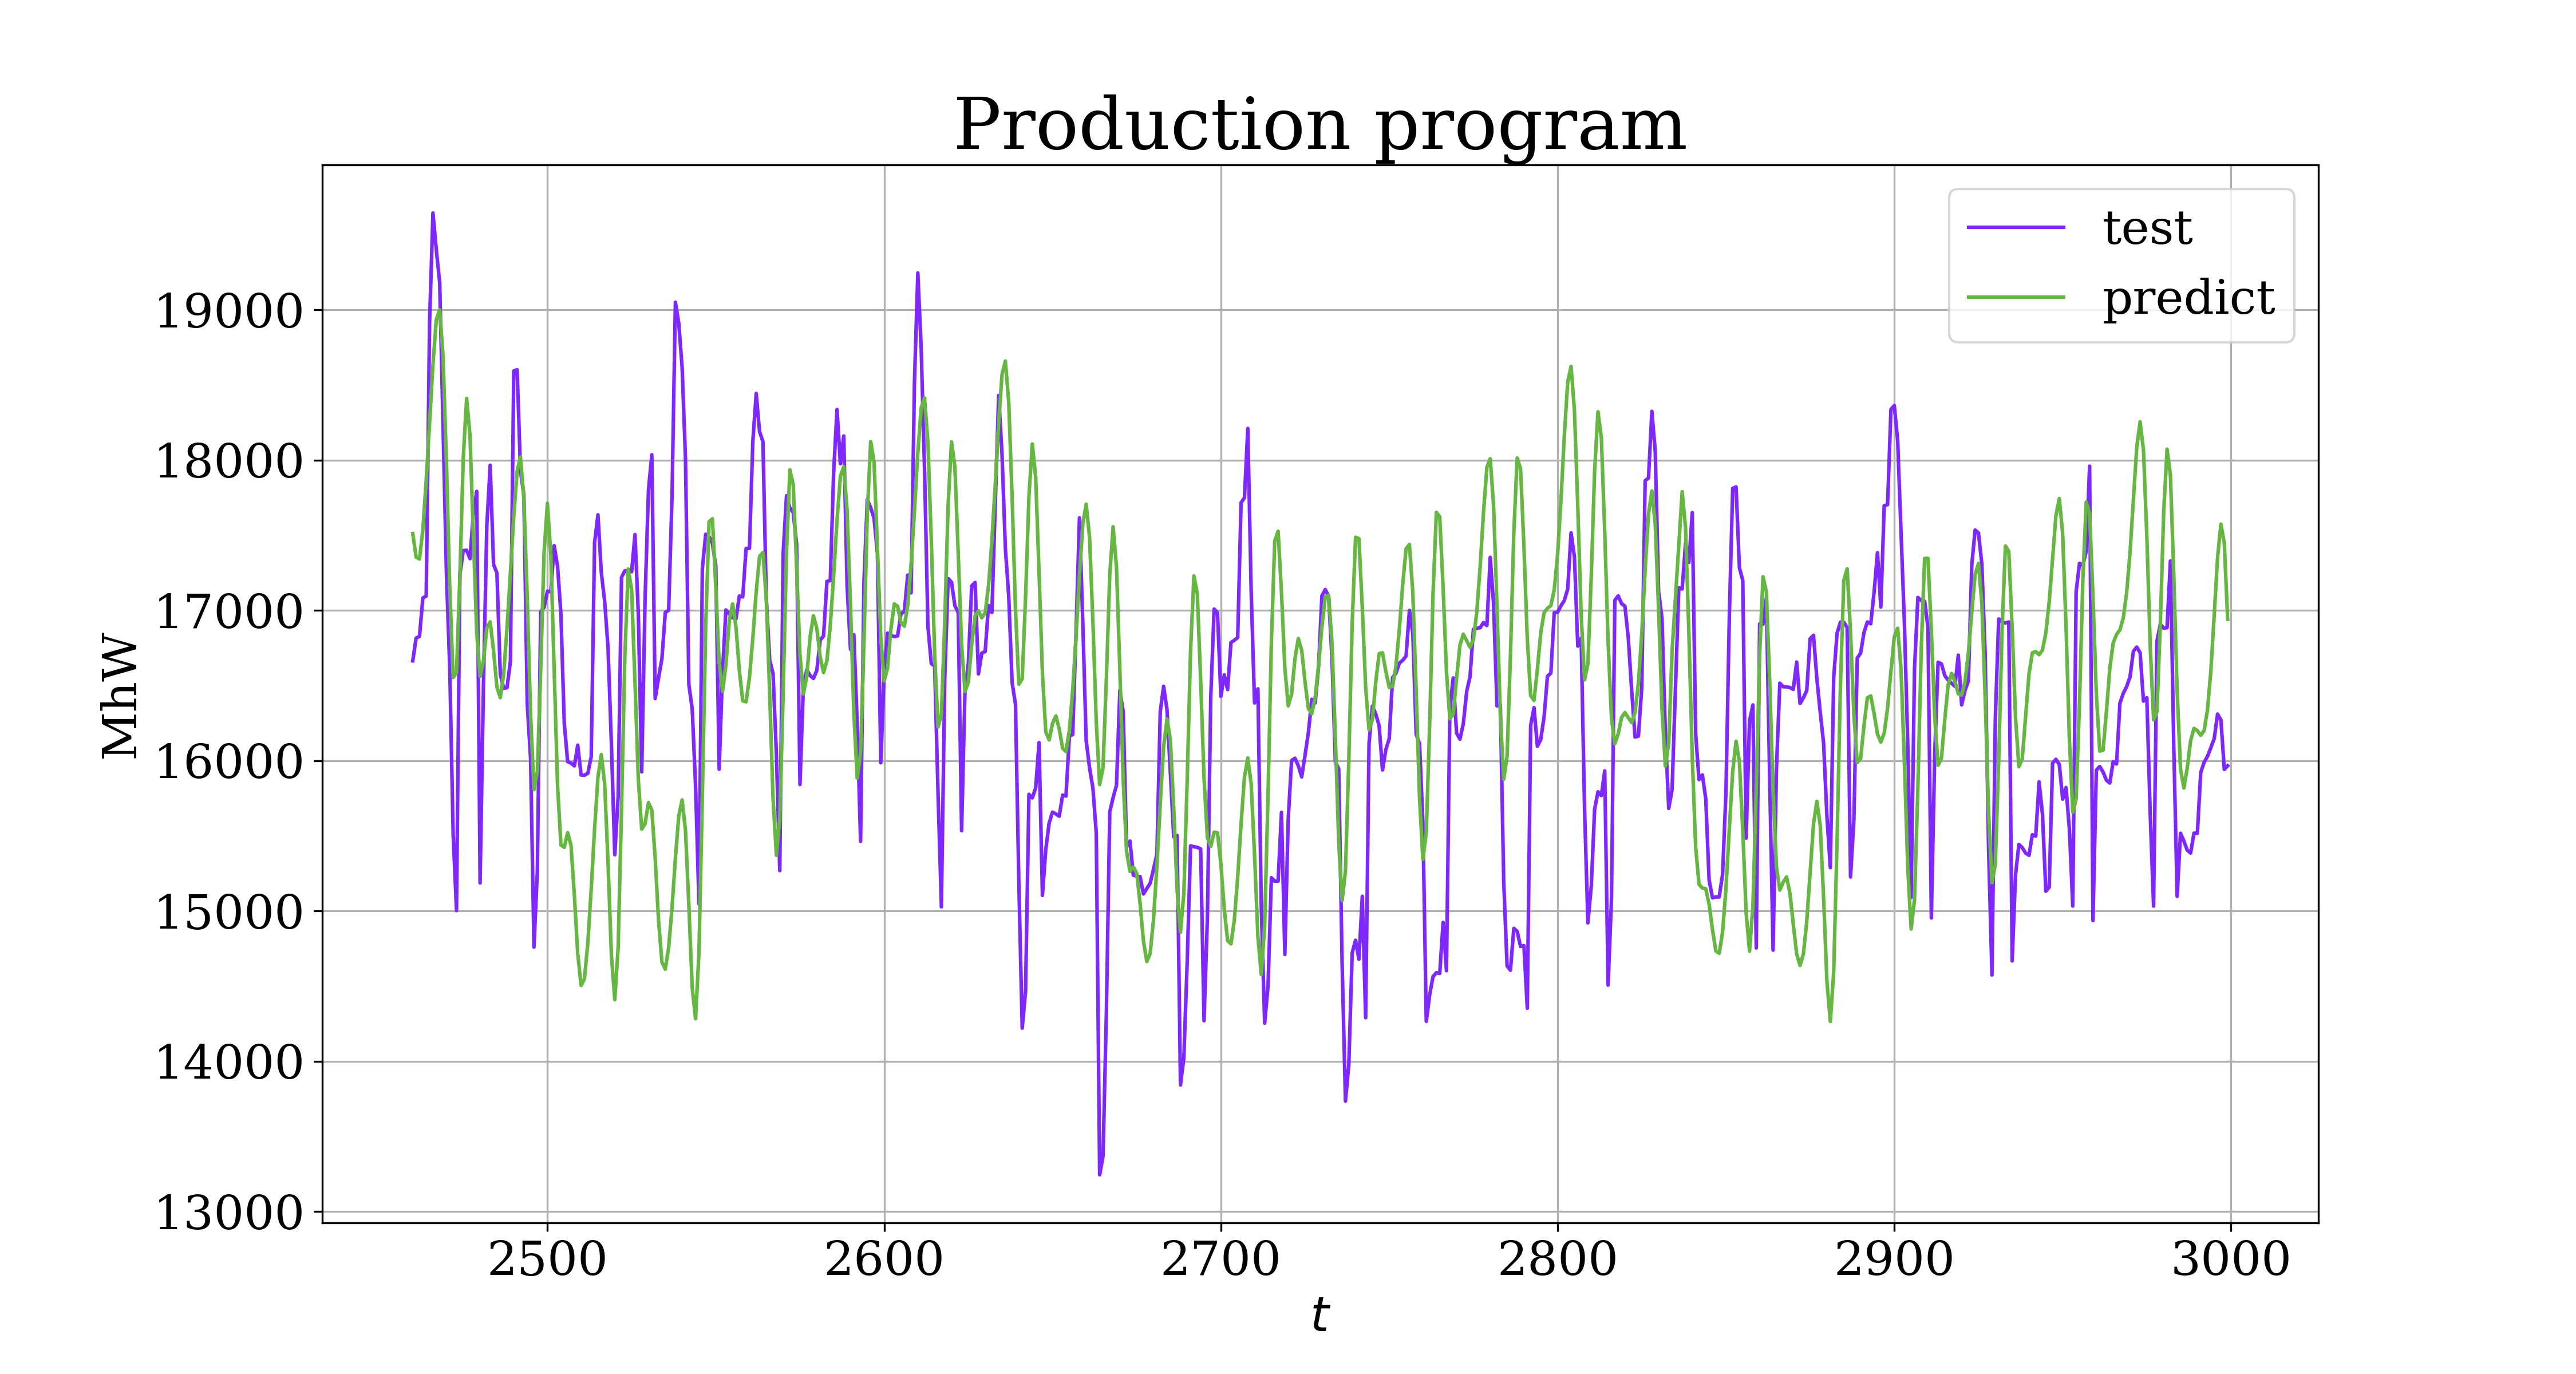
\includegraphics[width=0.48\textwidth, keepaspectratio]{../../experiments/electricity/tssa/figs/prediction/cpd_rank_30/Production_program.png}
			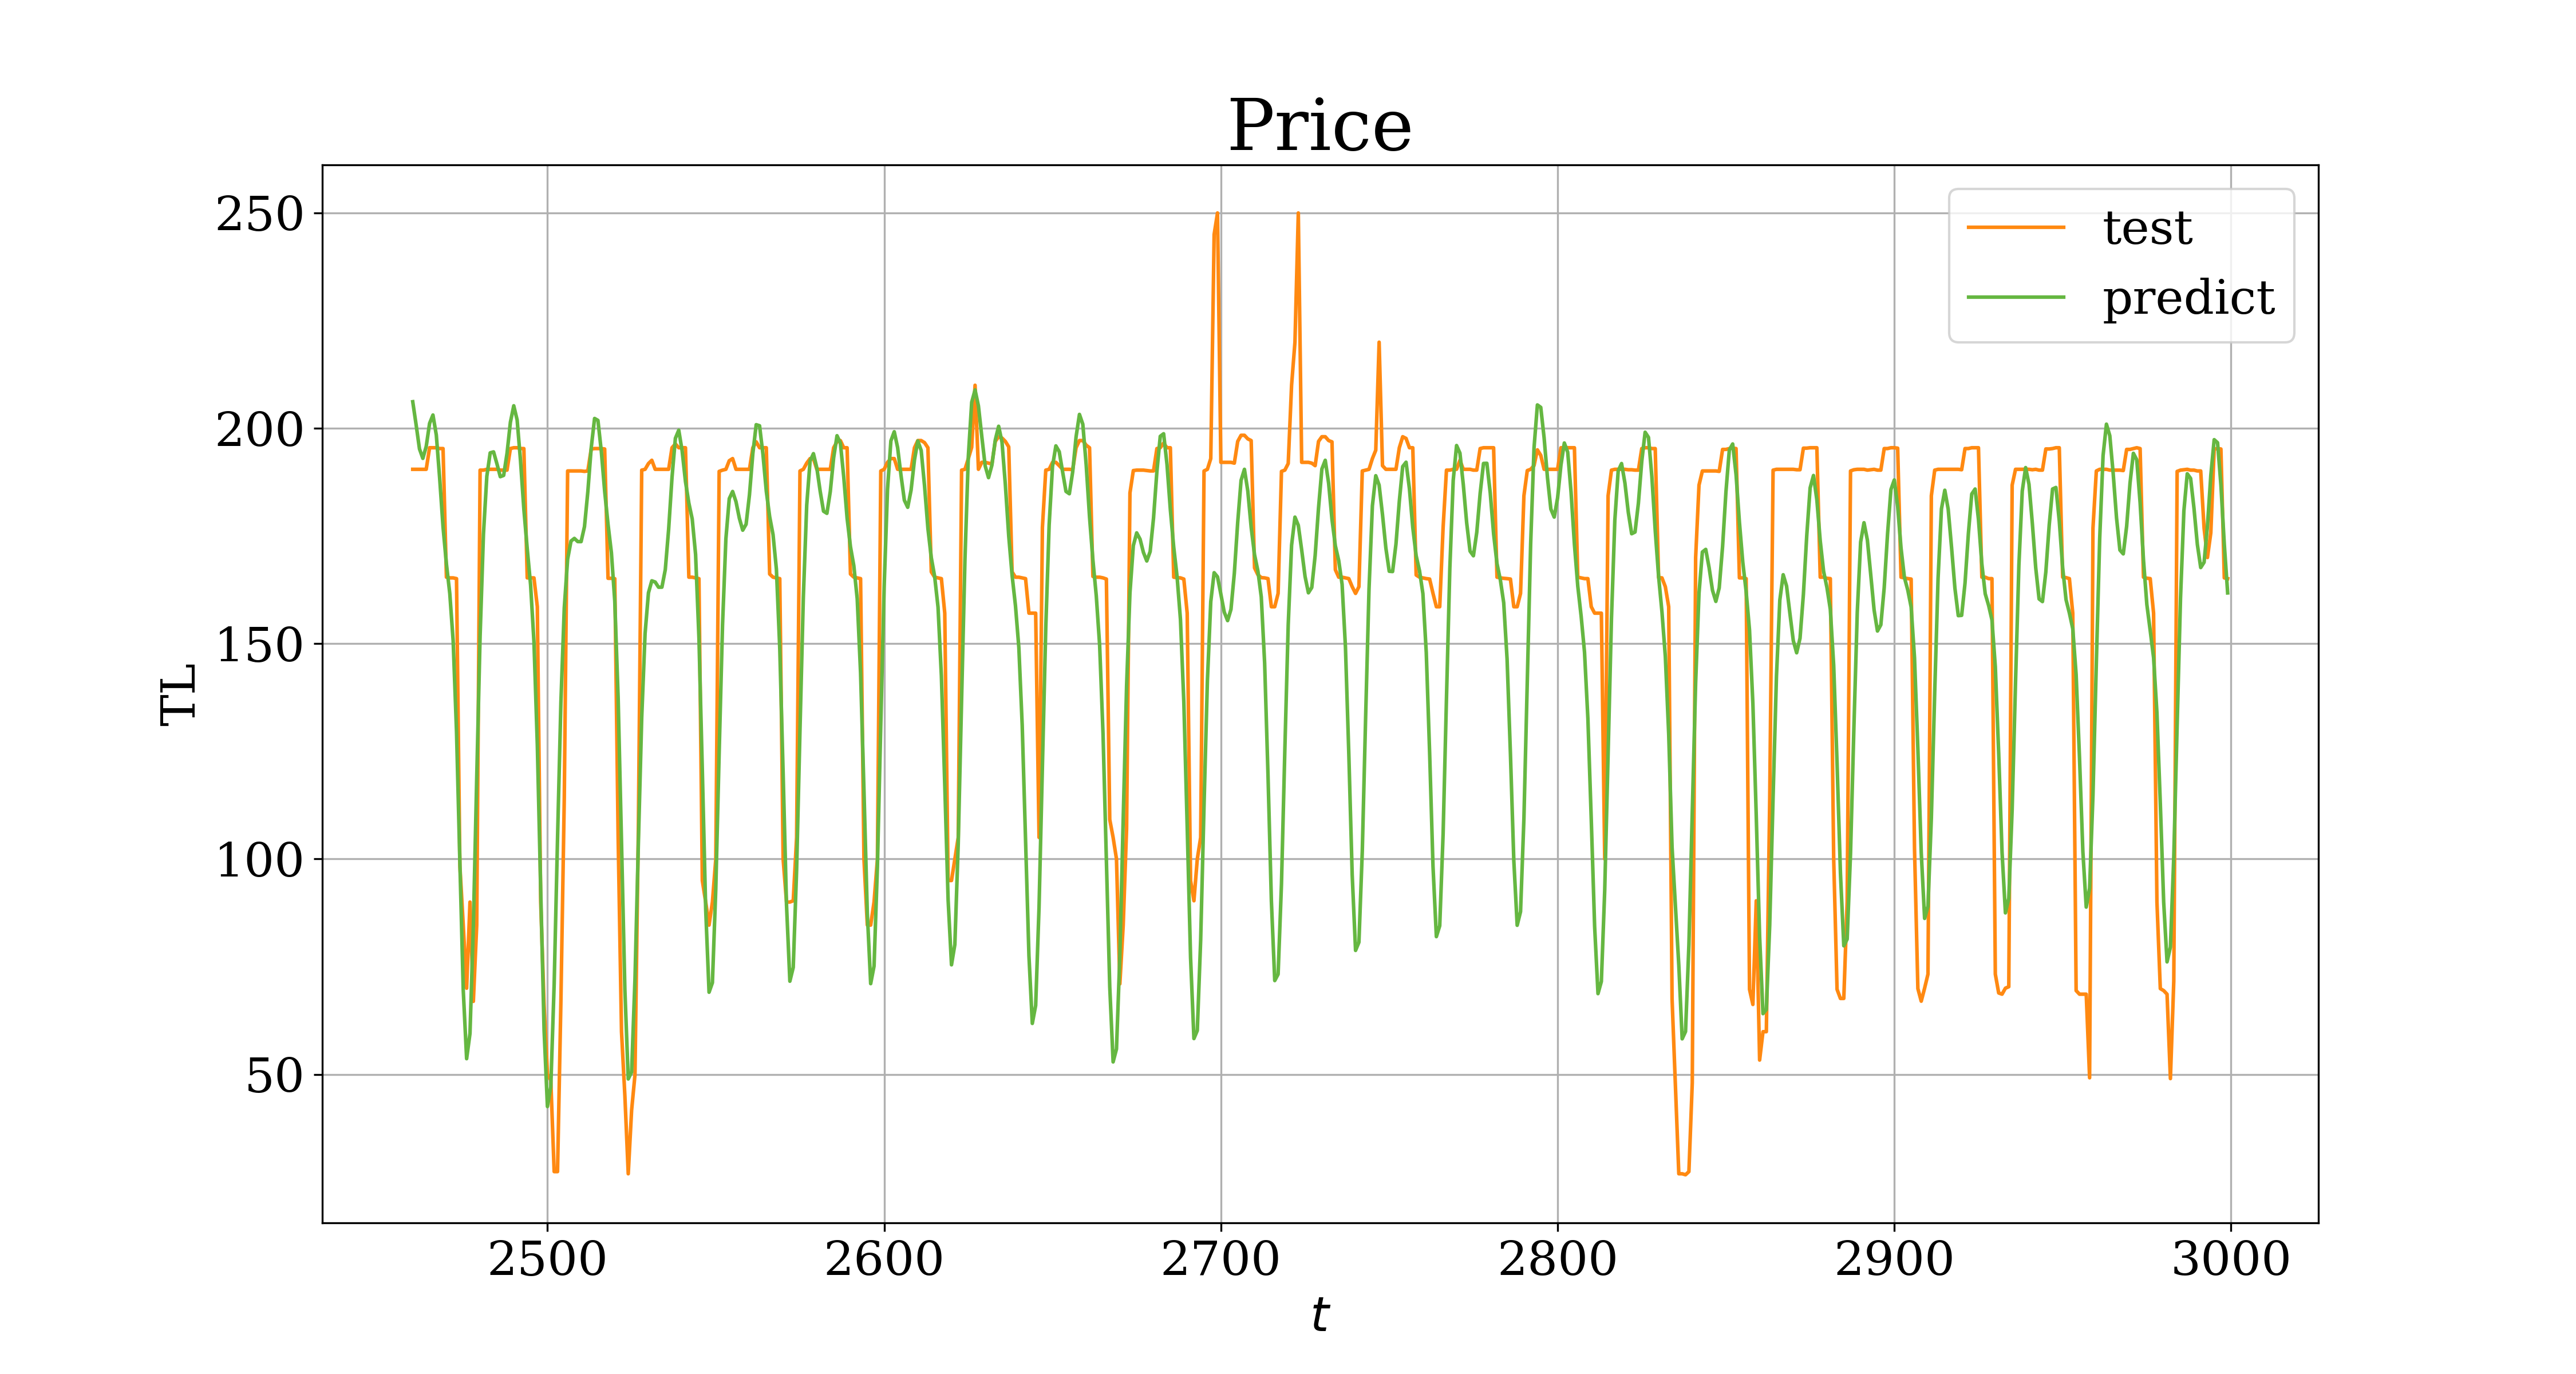
\includegraphics[width=0.48\textwidth, keepaspectratio]{../../experiments/electricity/tssa/figs/prediction/cpd_rank_30/Price.png}
			\caption{tSSA forecast for electricity data. CPD rank $ = 30 $}\label{fig:tssa_electr_pred}
		\end{figure}
		
		\begin{figure}[h]
			\centering
			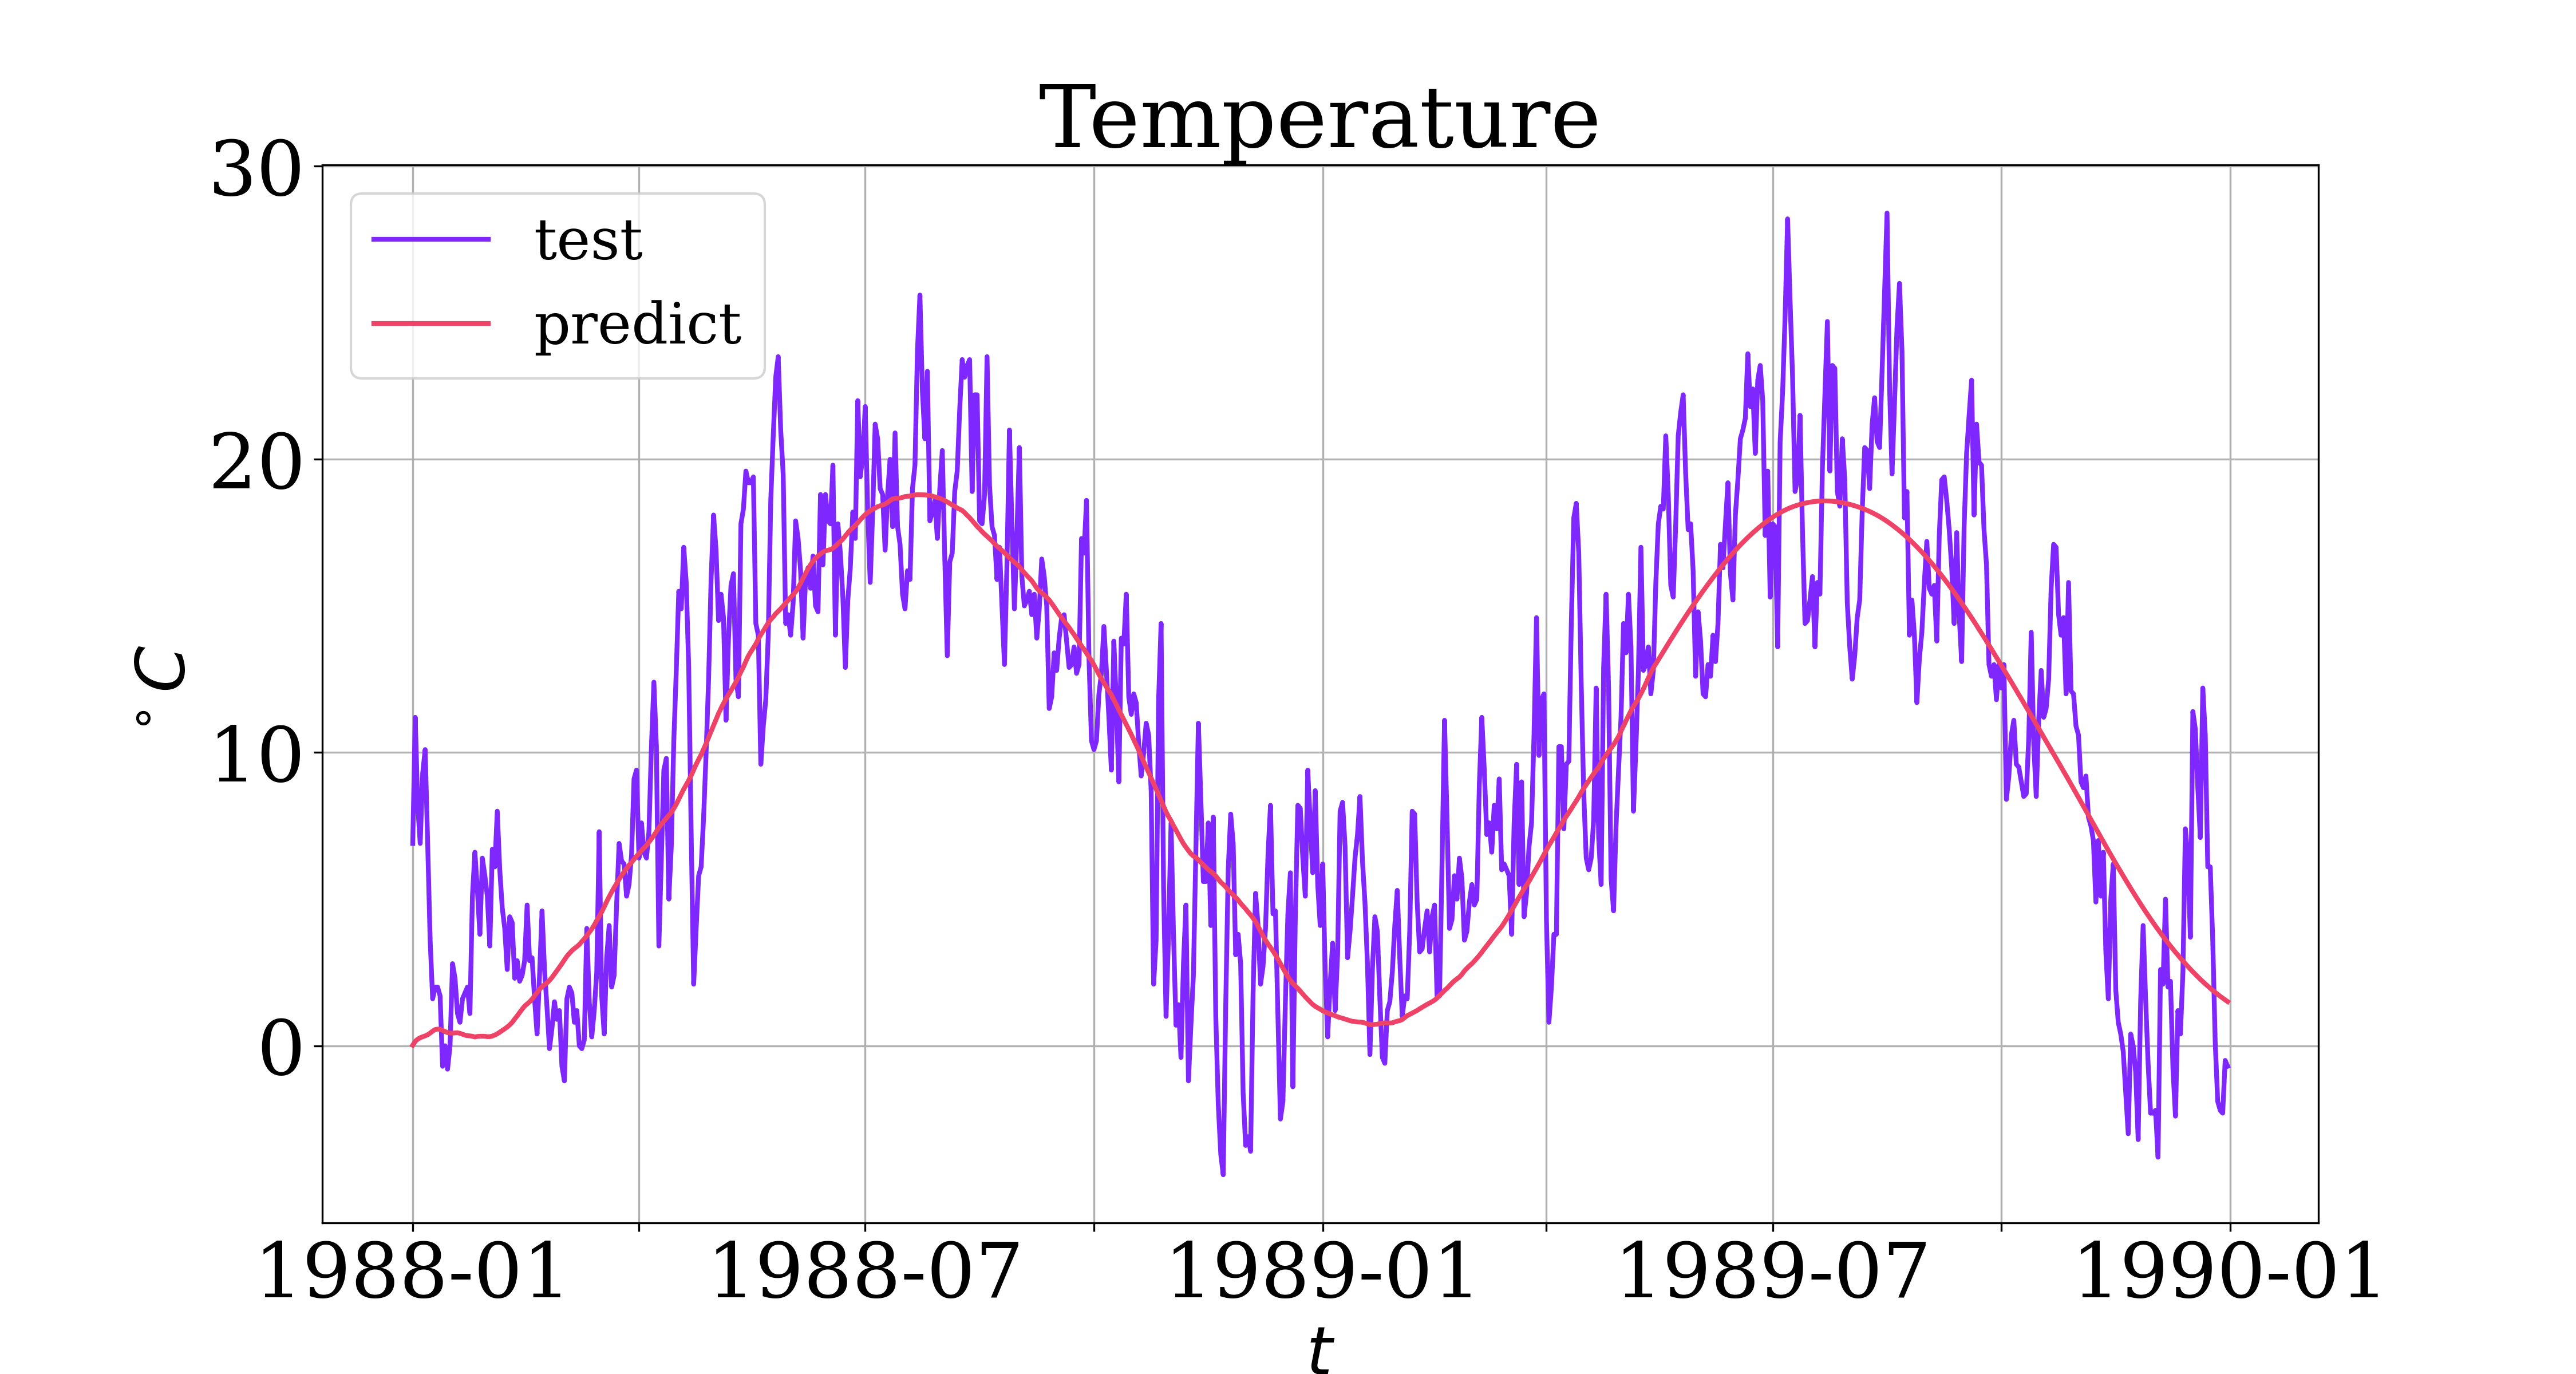
\includegraphics[width=0.48\textwidth, keepaspectratio]{../../experiments/weather/tssa/figs/prediction/cpd_rank_5/Temperature.png}
			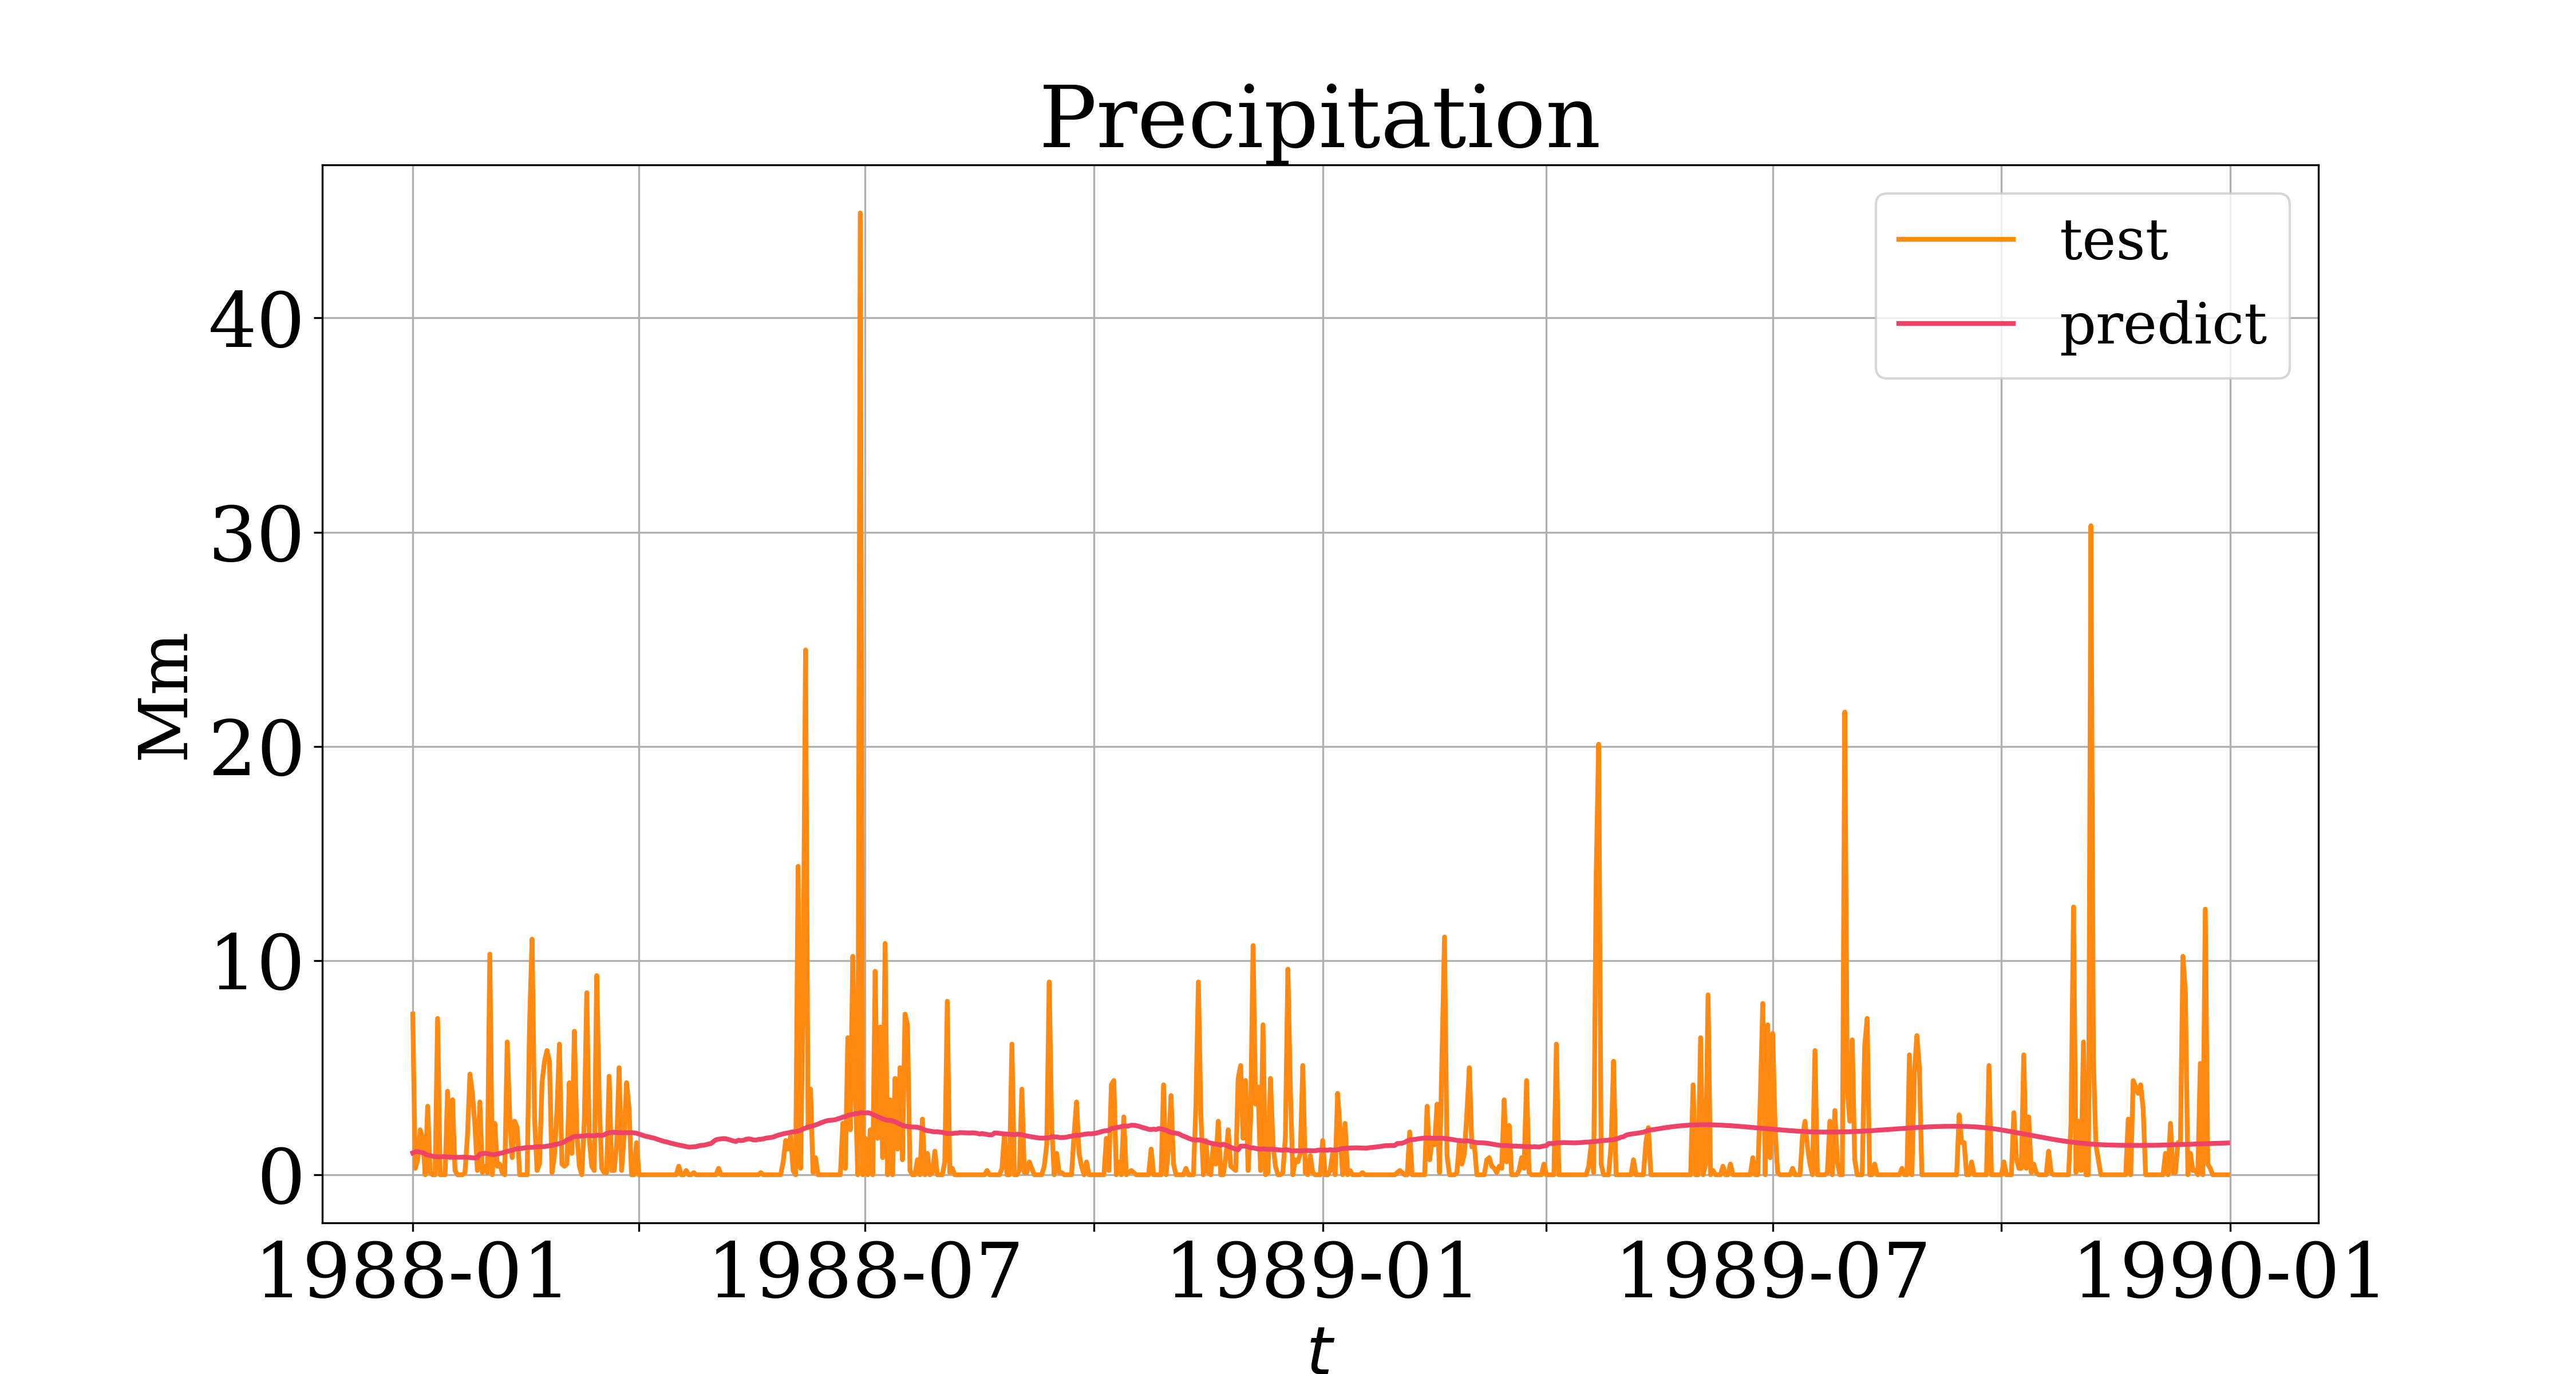
\includegraphics[width=0.48\textwidth, keepaspectratio]{../../experiments/weather/tssa/figs/prediction/cpd_rank_5/Precipitation.png}
			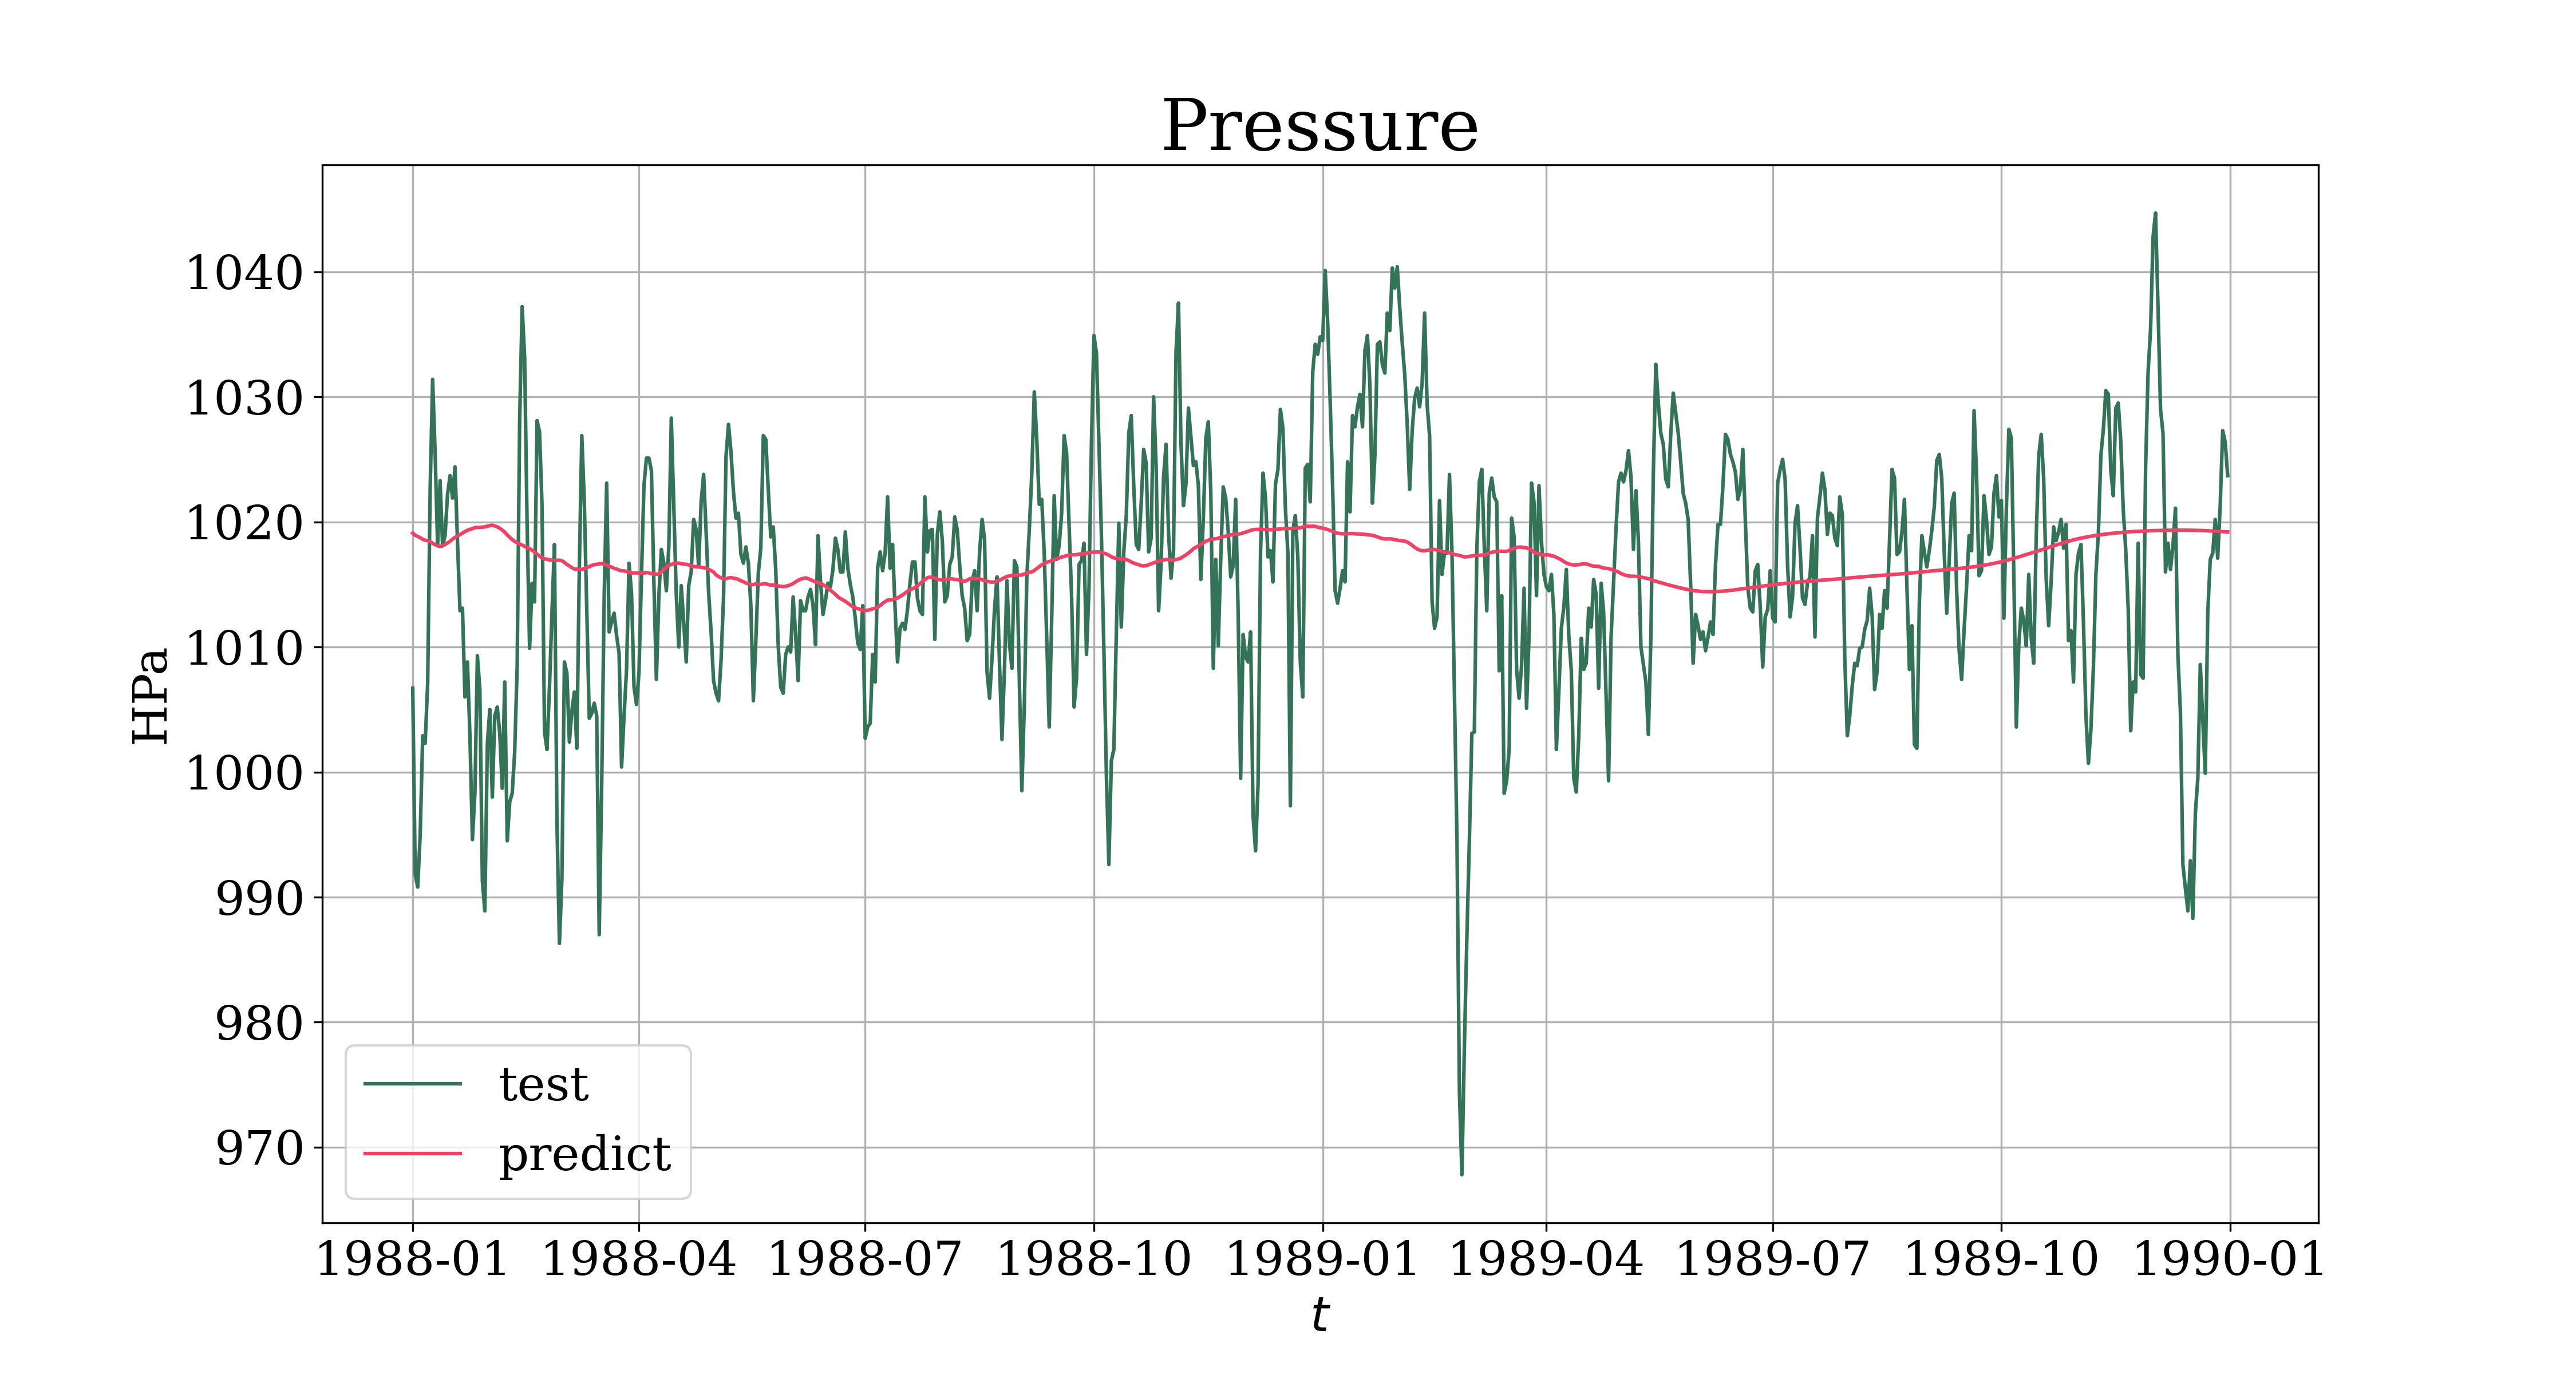
\includegraphics[width=0.48\textwidth, keepaspectratio]{../../experiments/weather/tssa/figs/prediction/cpd_rank_5/Pressure.png}
			\caption{tSSA forecast for weather data. CPD rank $ = 5 $}\label{fig:tssa_weather_pred}
		\end{figure}
		
		\begin{figure}[h]
			\centering
			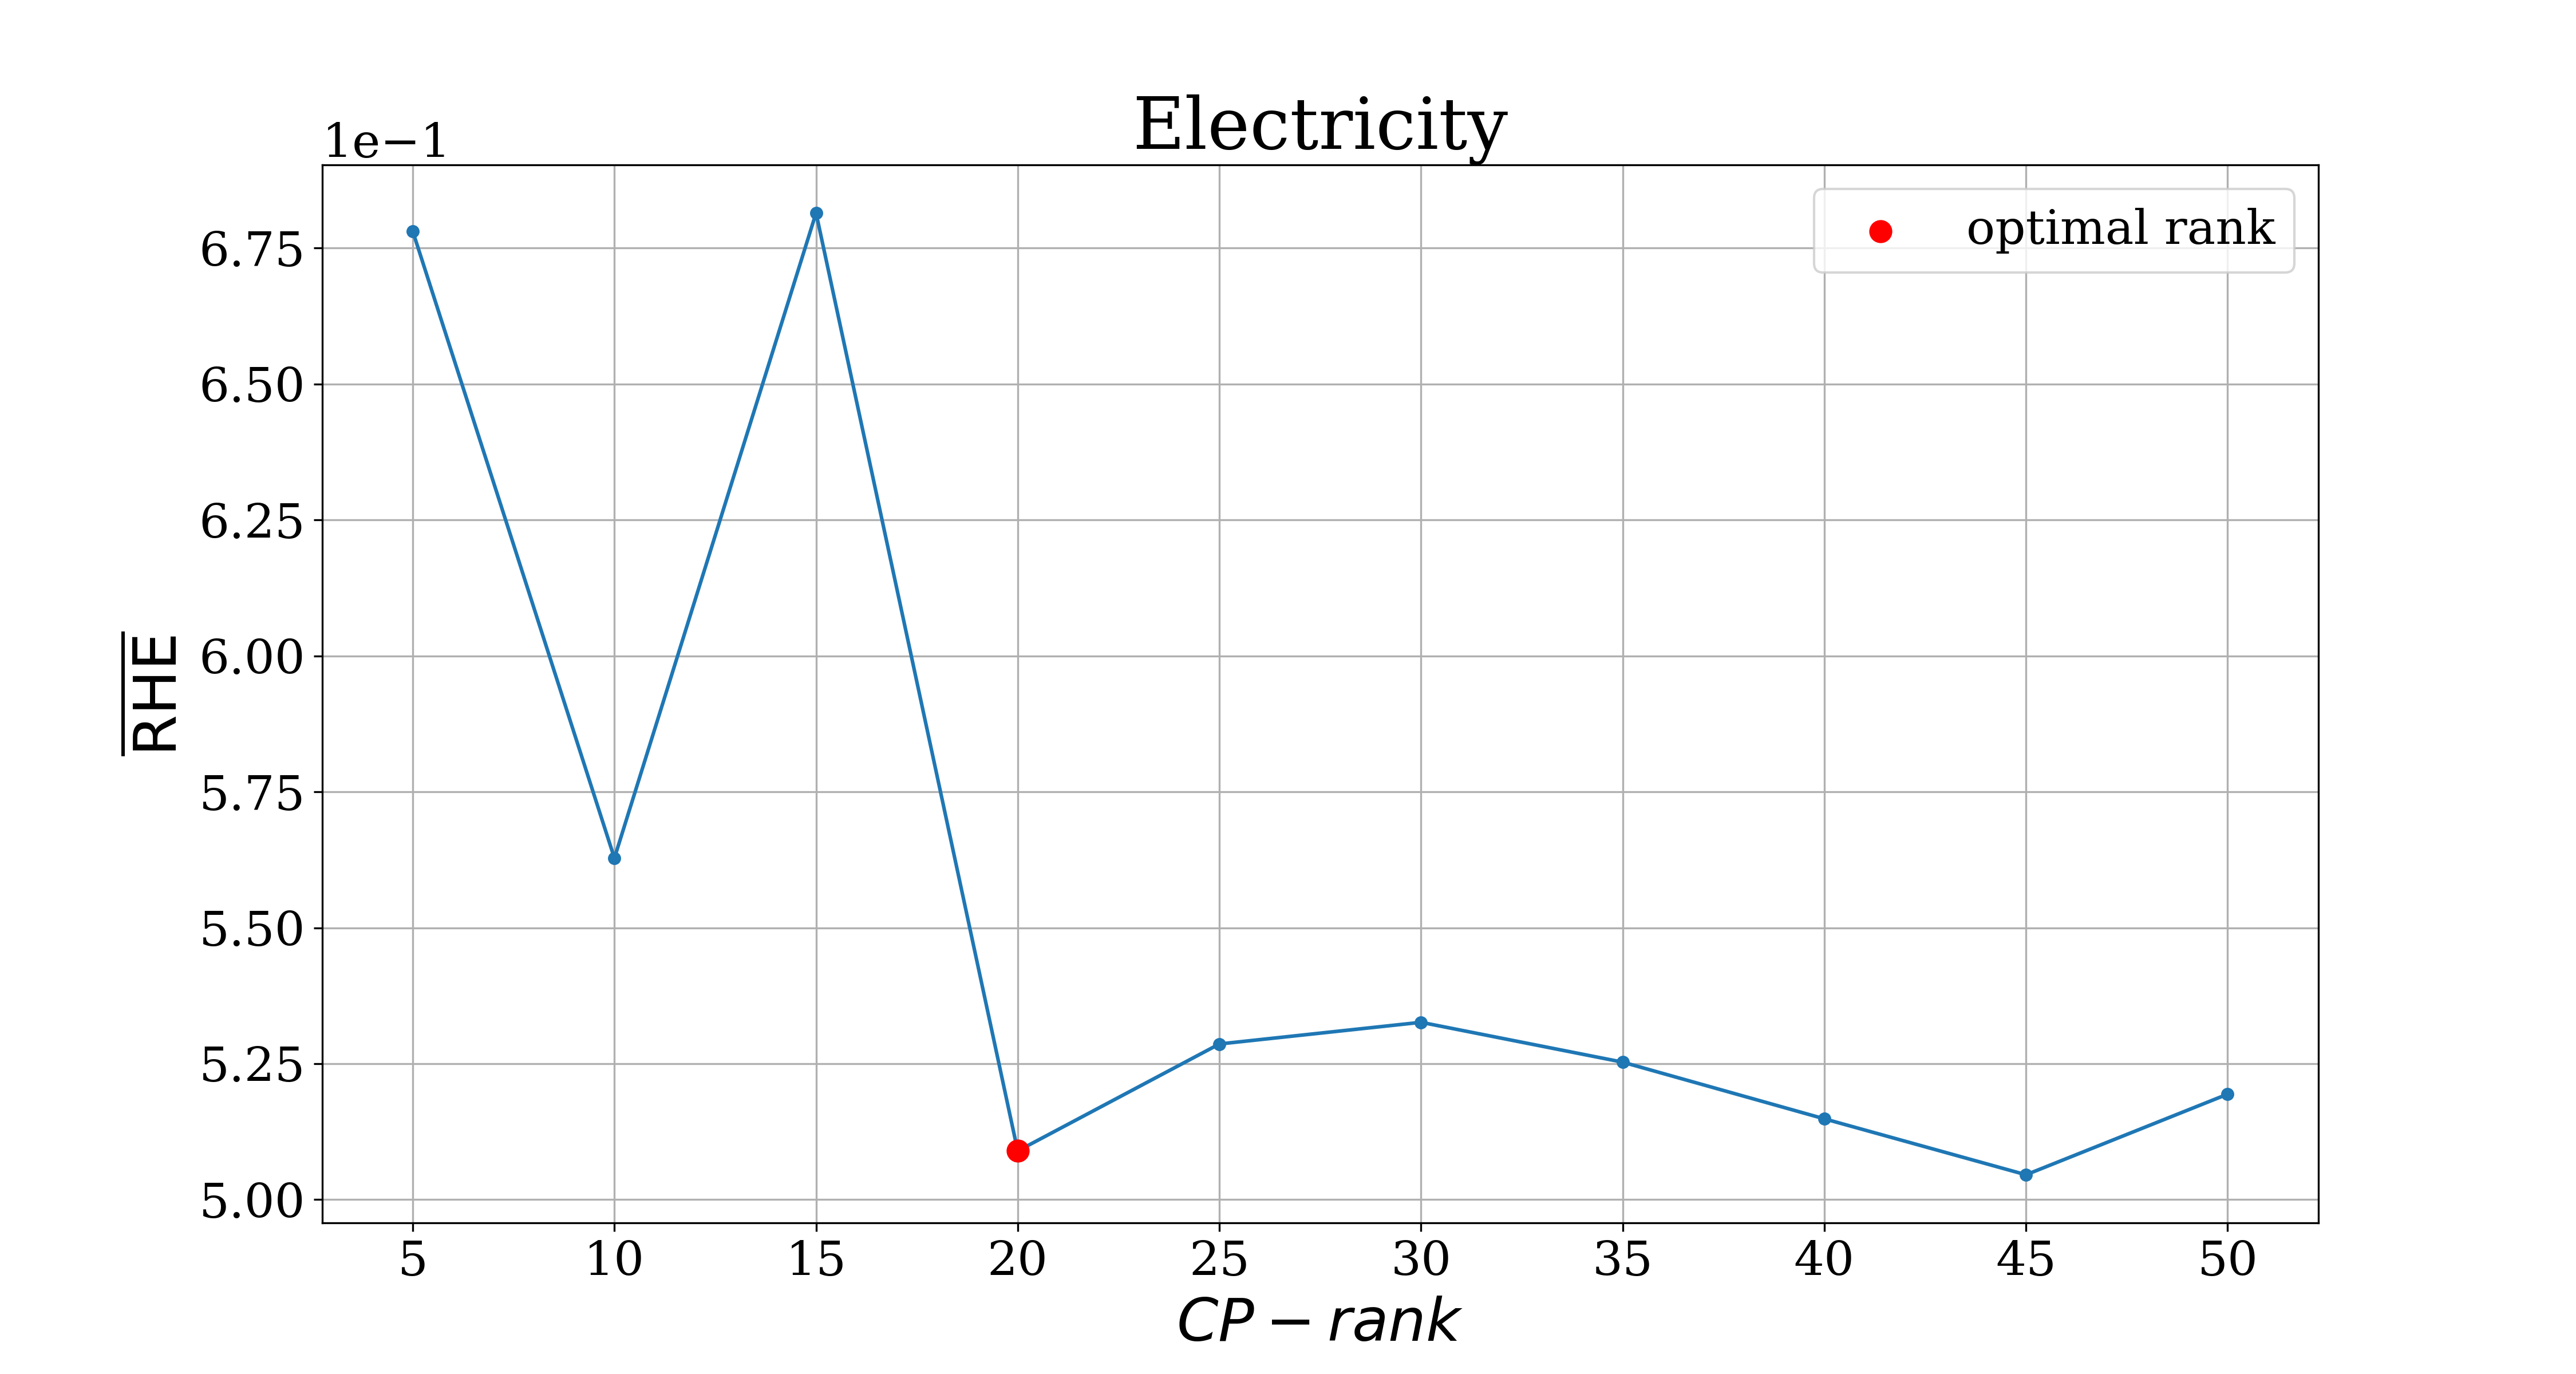
\includegraphics[width=0.48\textwidth, keepaspectratio]{../../experiments/electricity/tssa/figs/decomposition/RHE_mean.png}
			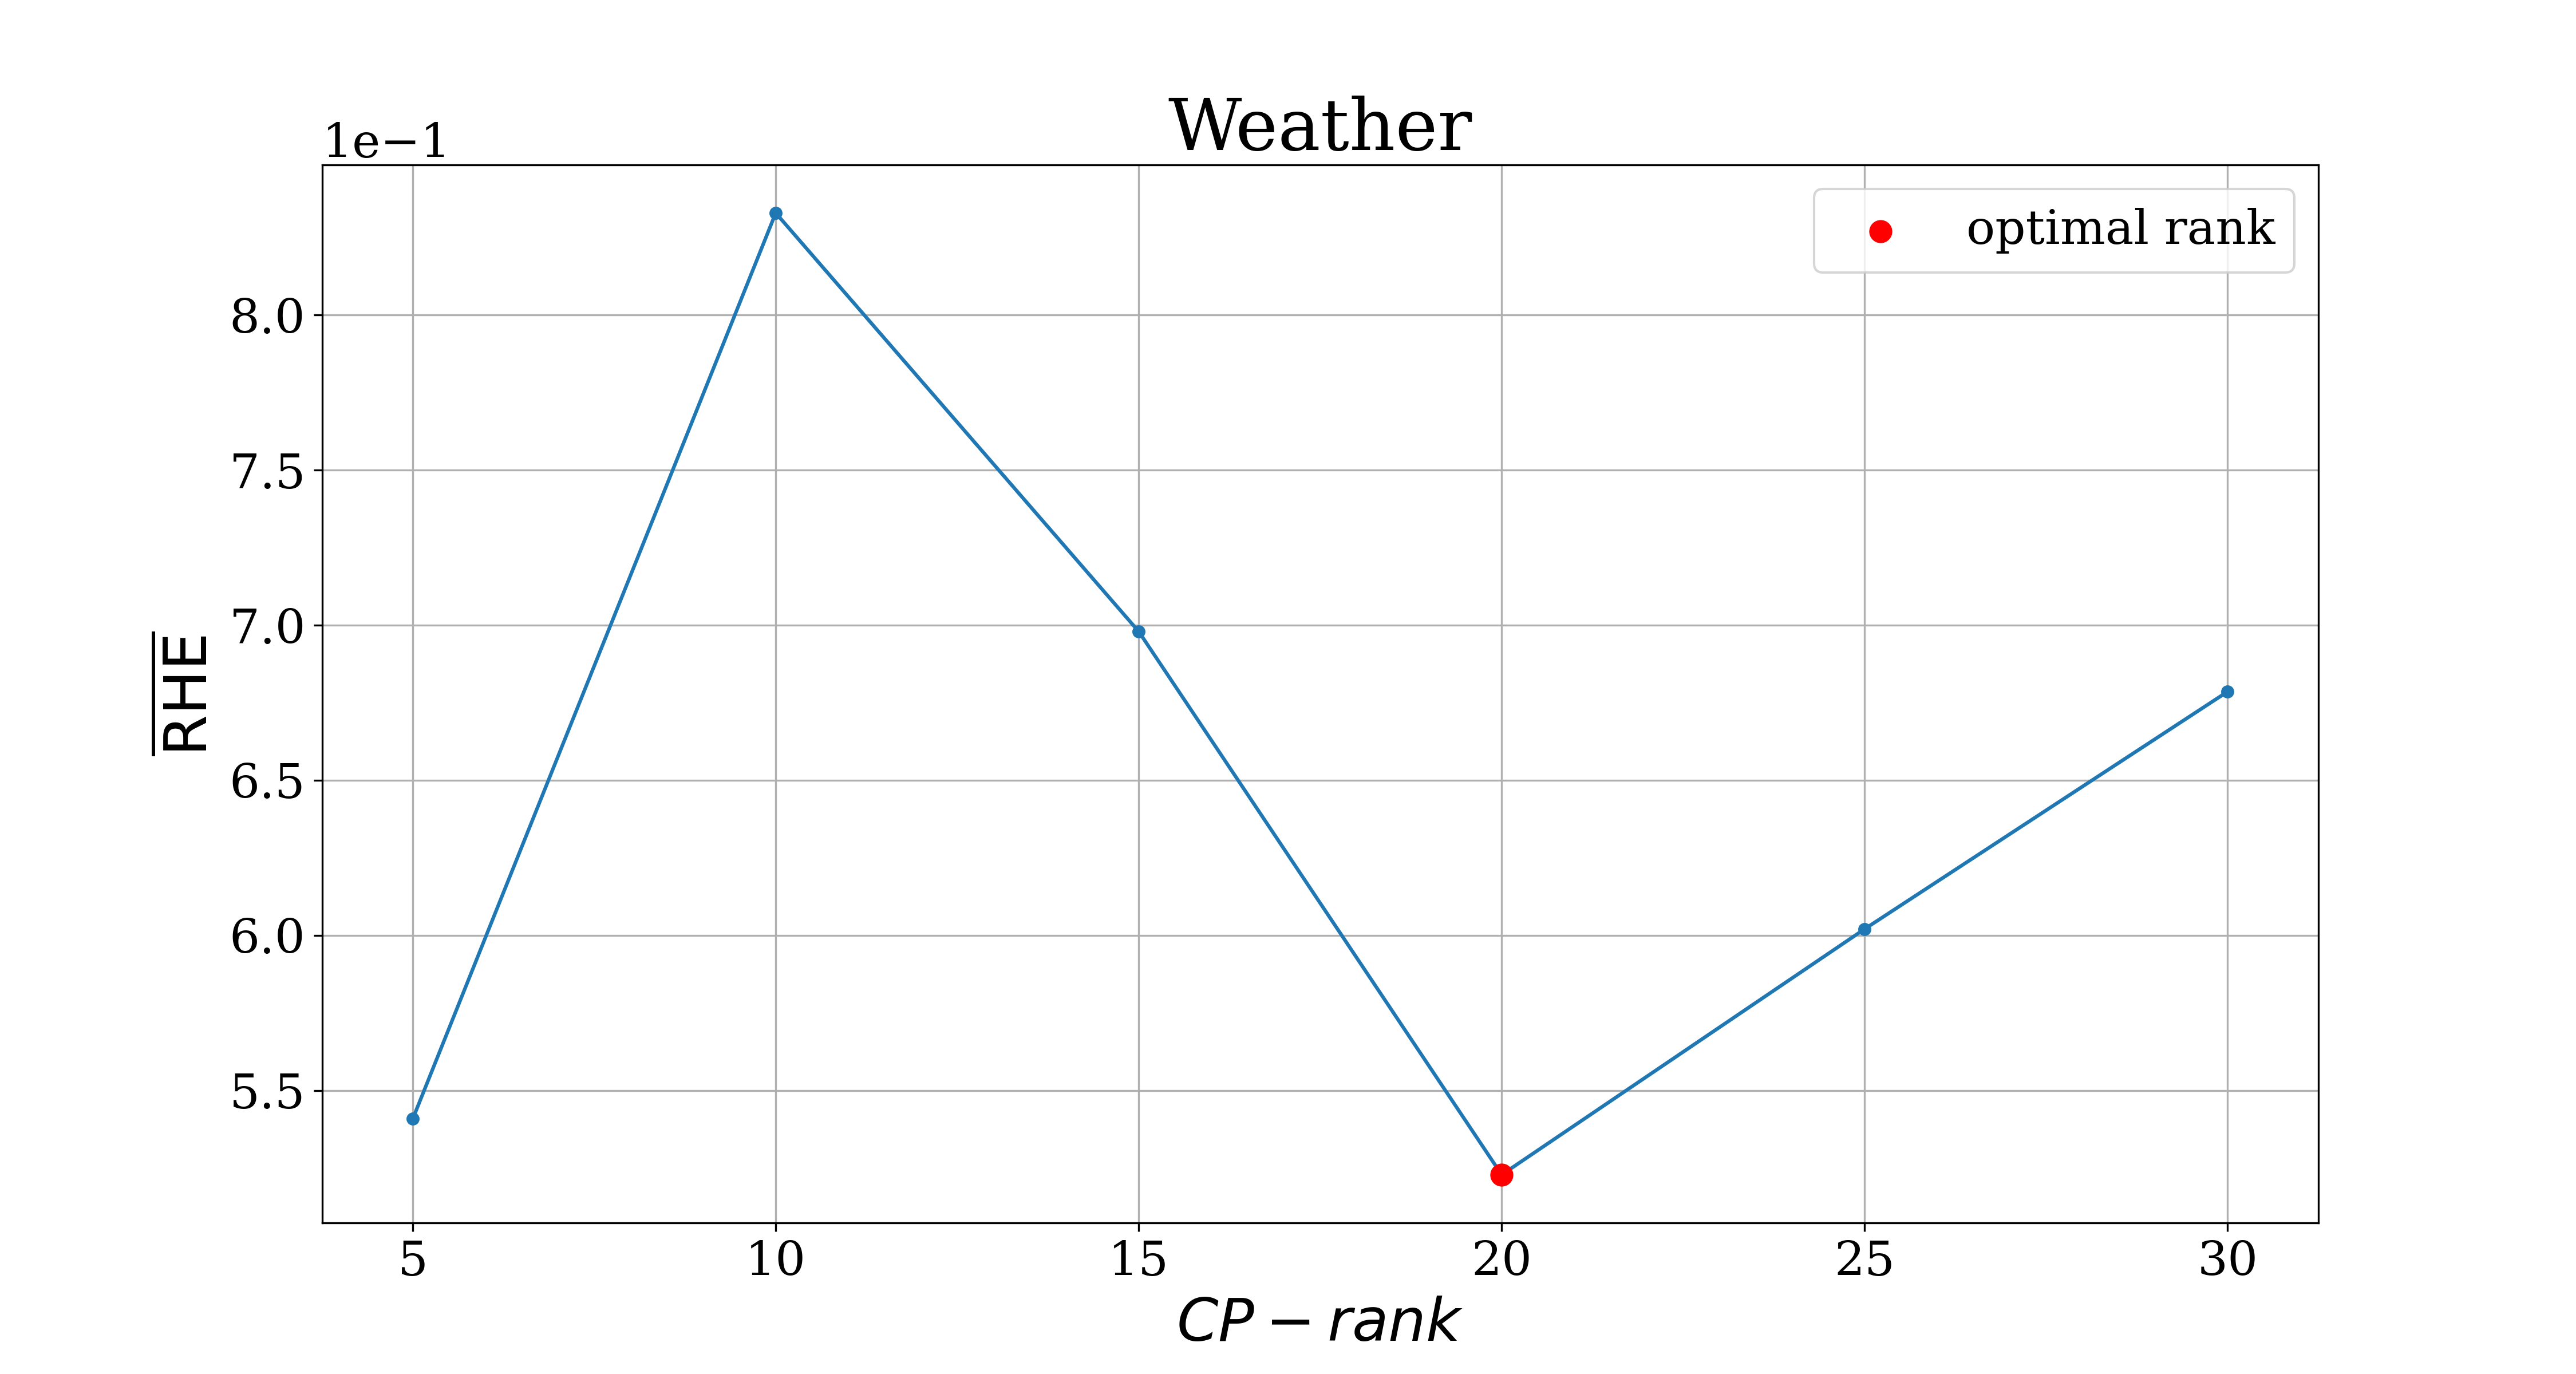
\includegraphics[width=0.48\textwidth, keepaspectratio]{../../experiments/weather/tssa/figs/decomposition/RHE_mean.png}
			\caption{Relation between $ \overline{\text{RHE}} $ metrics and CPD rank. The left is for electricity data, the right is for weather data. Optimal point is marked with red}\label{fig:decomp_rhe_rank}
		\end{figure}
		
		\begin{figure}[h]
			\centering
			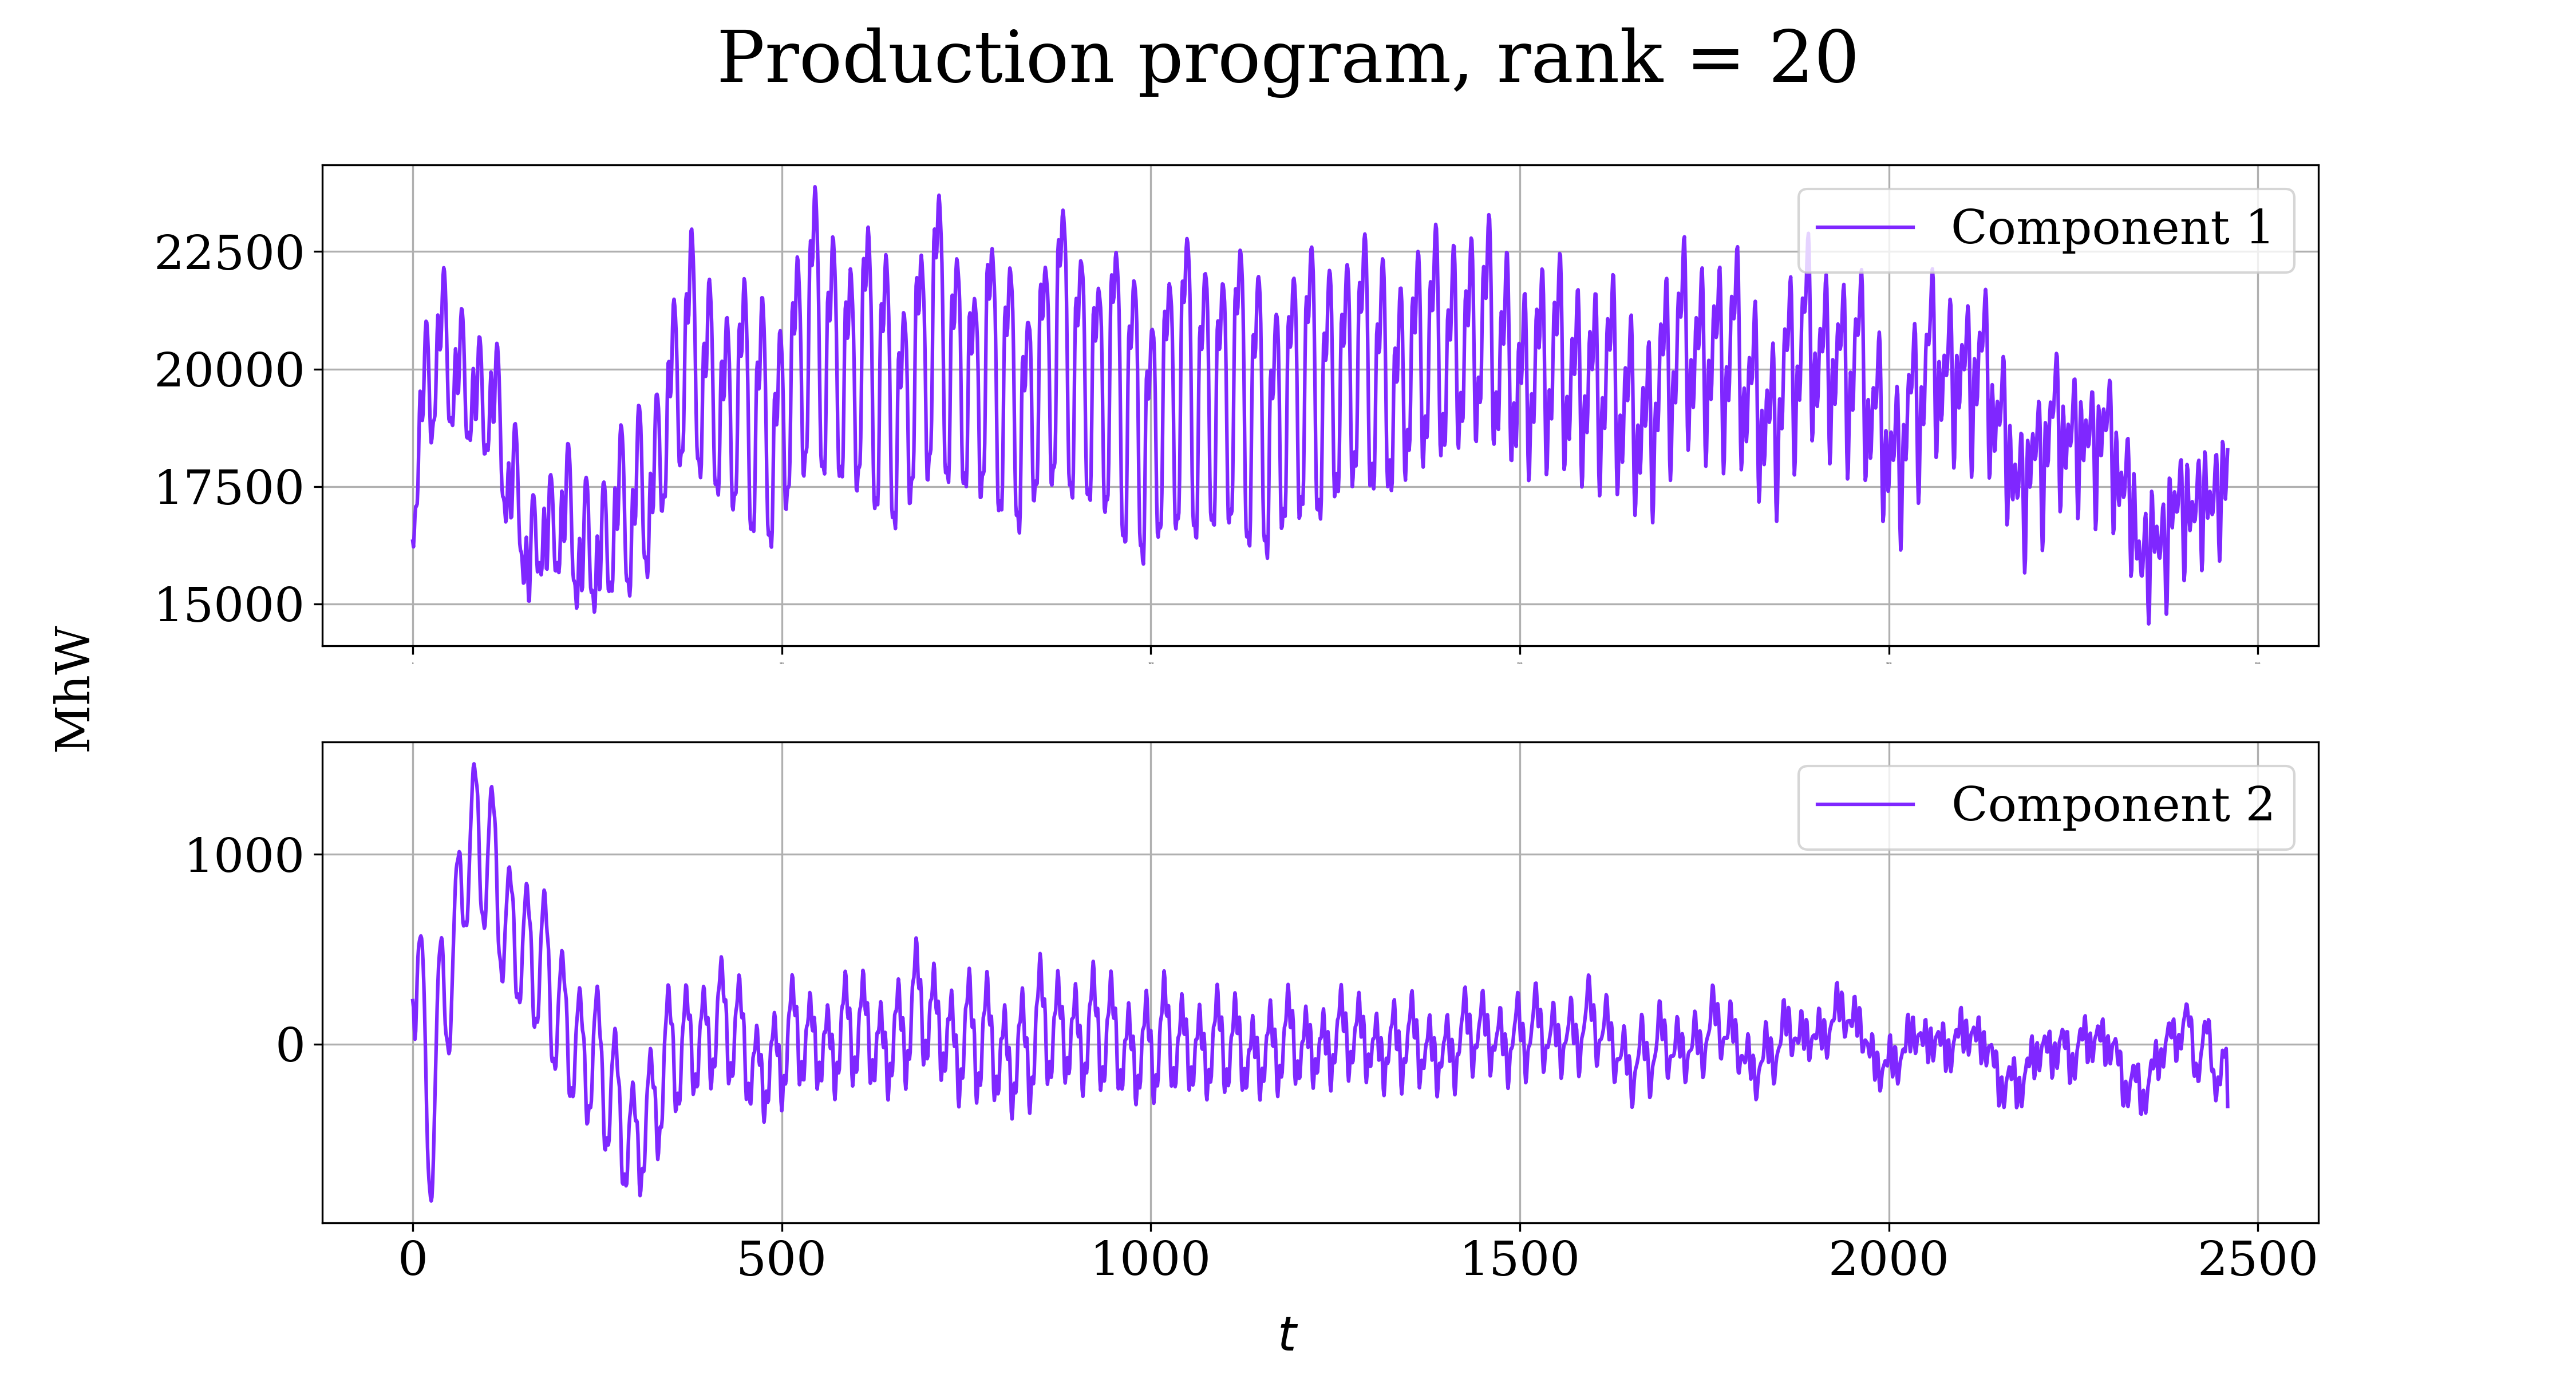
\includegraphics[width=0.48\textwidth, keepaspectratio]{../../experiments/electricity/tssa/figs/decomposition/cpd_rank_20/Production_program.png}
			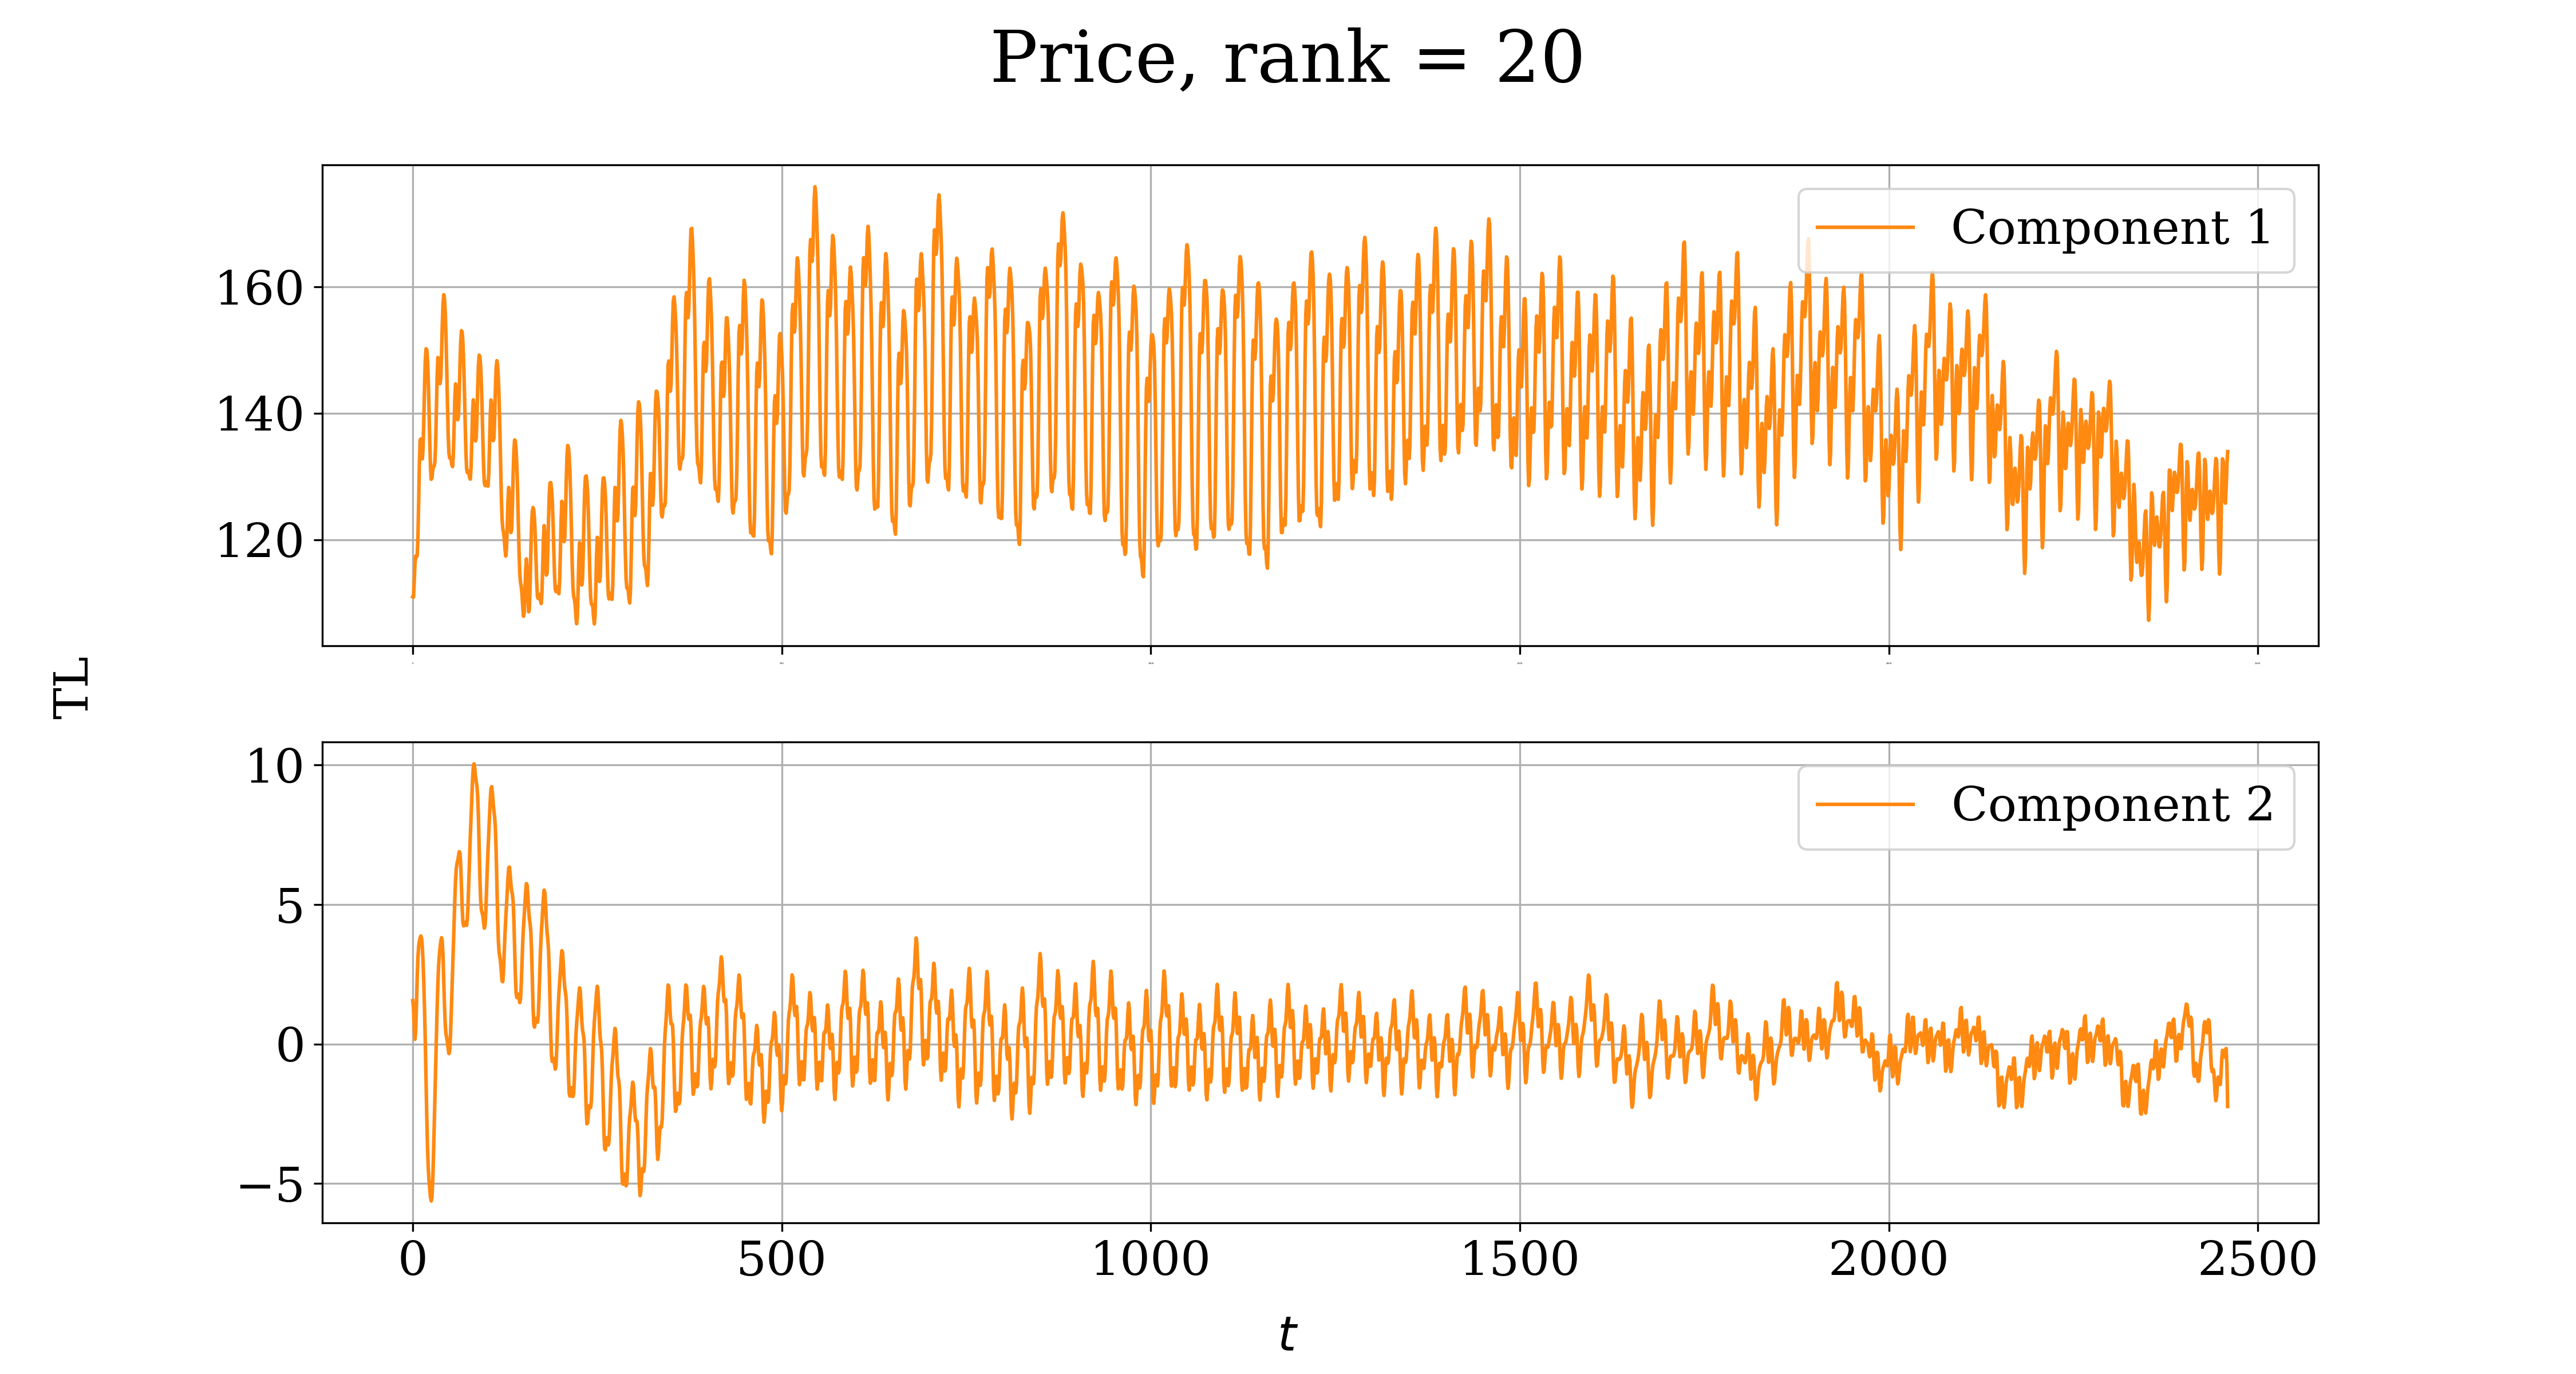
\includegraphics[width=0.48\textwidth, keepaspectratio]{../../experiments/electricity/tssa/figs/decomposition/cpd_rank_20/Price.png}
			\caption{tSSA decomposition for electricity data. CPD rank $ = 20 $}\label{fig:electr_decomp_tssa}
		\end{figure}
		
		\begin{figure}[h]
			\centering
			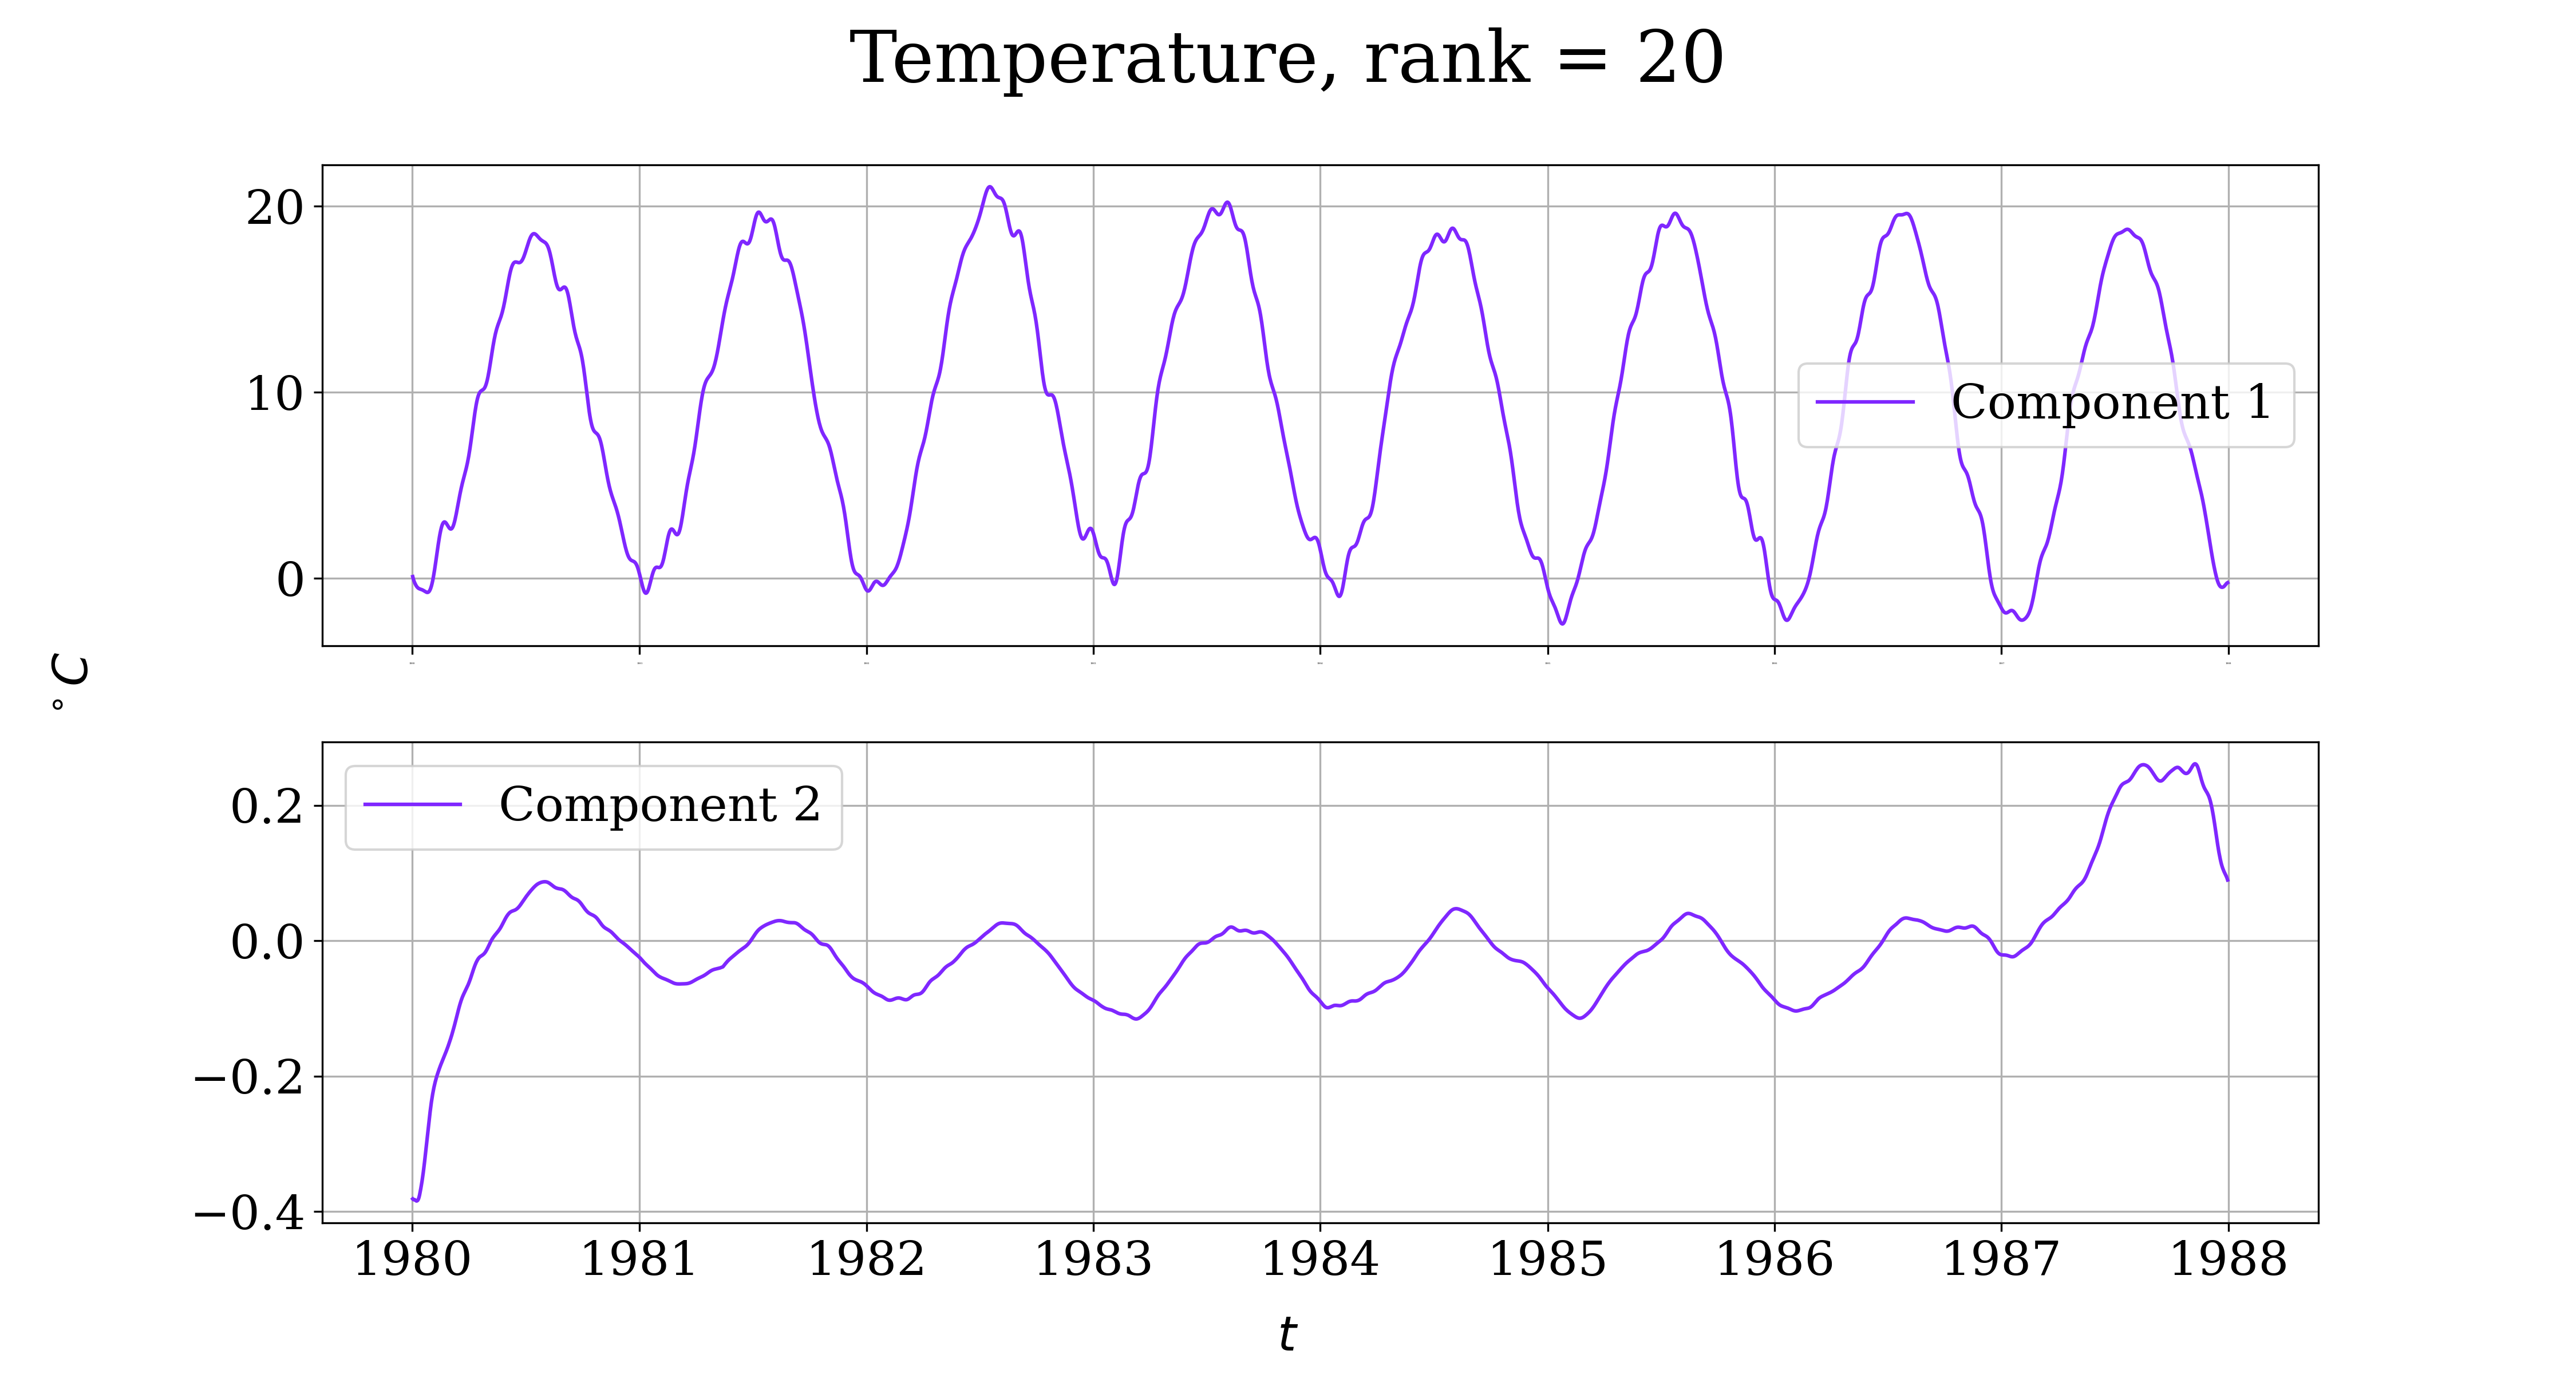
\includegraphics[width=0.48\textwidth, keepaspectratio]{../../experiments/weather/tssa/figs/decomposition/cpd_rank_20/Temperature.png}
			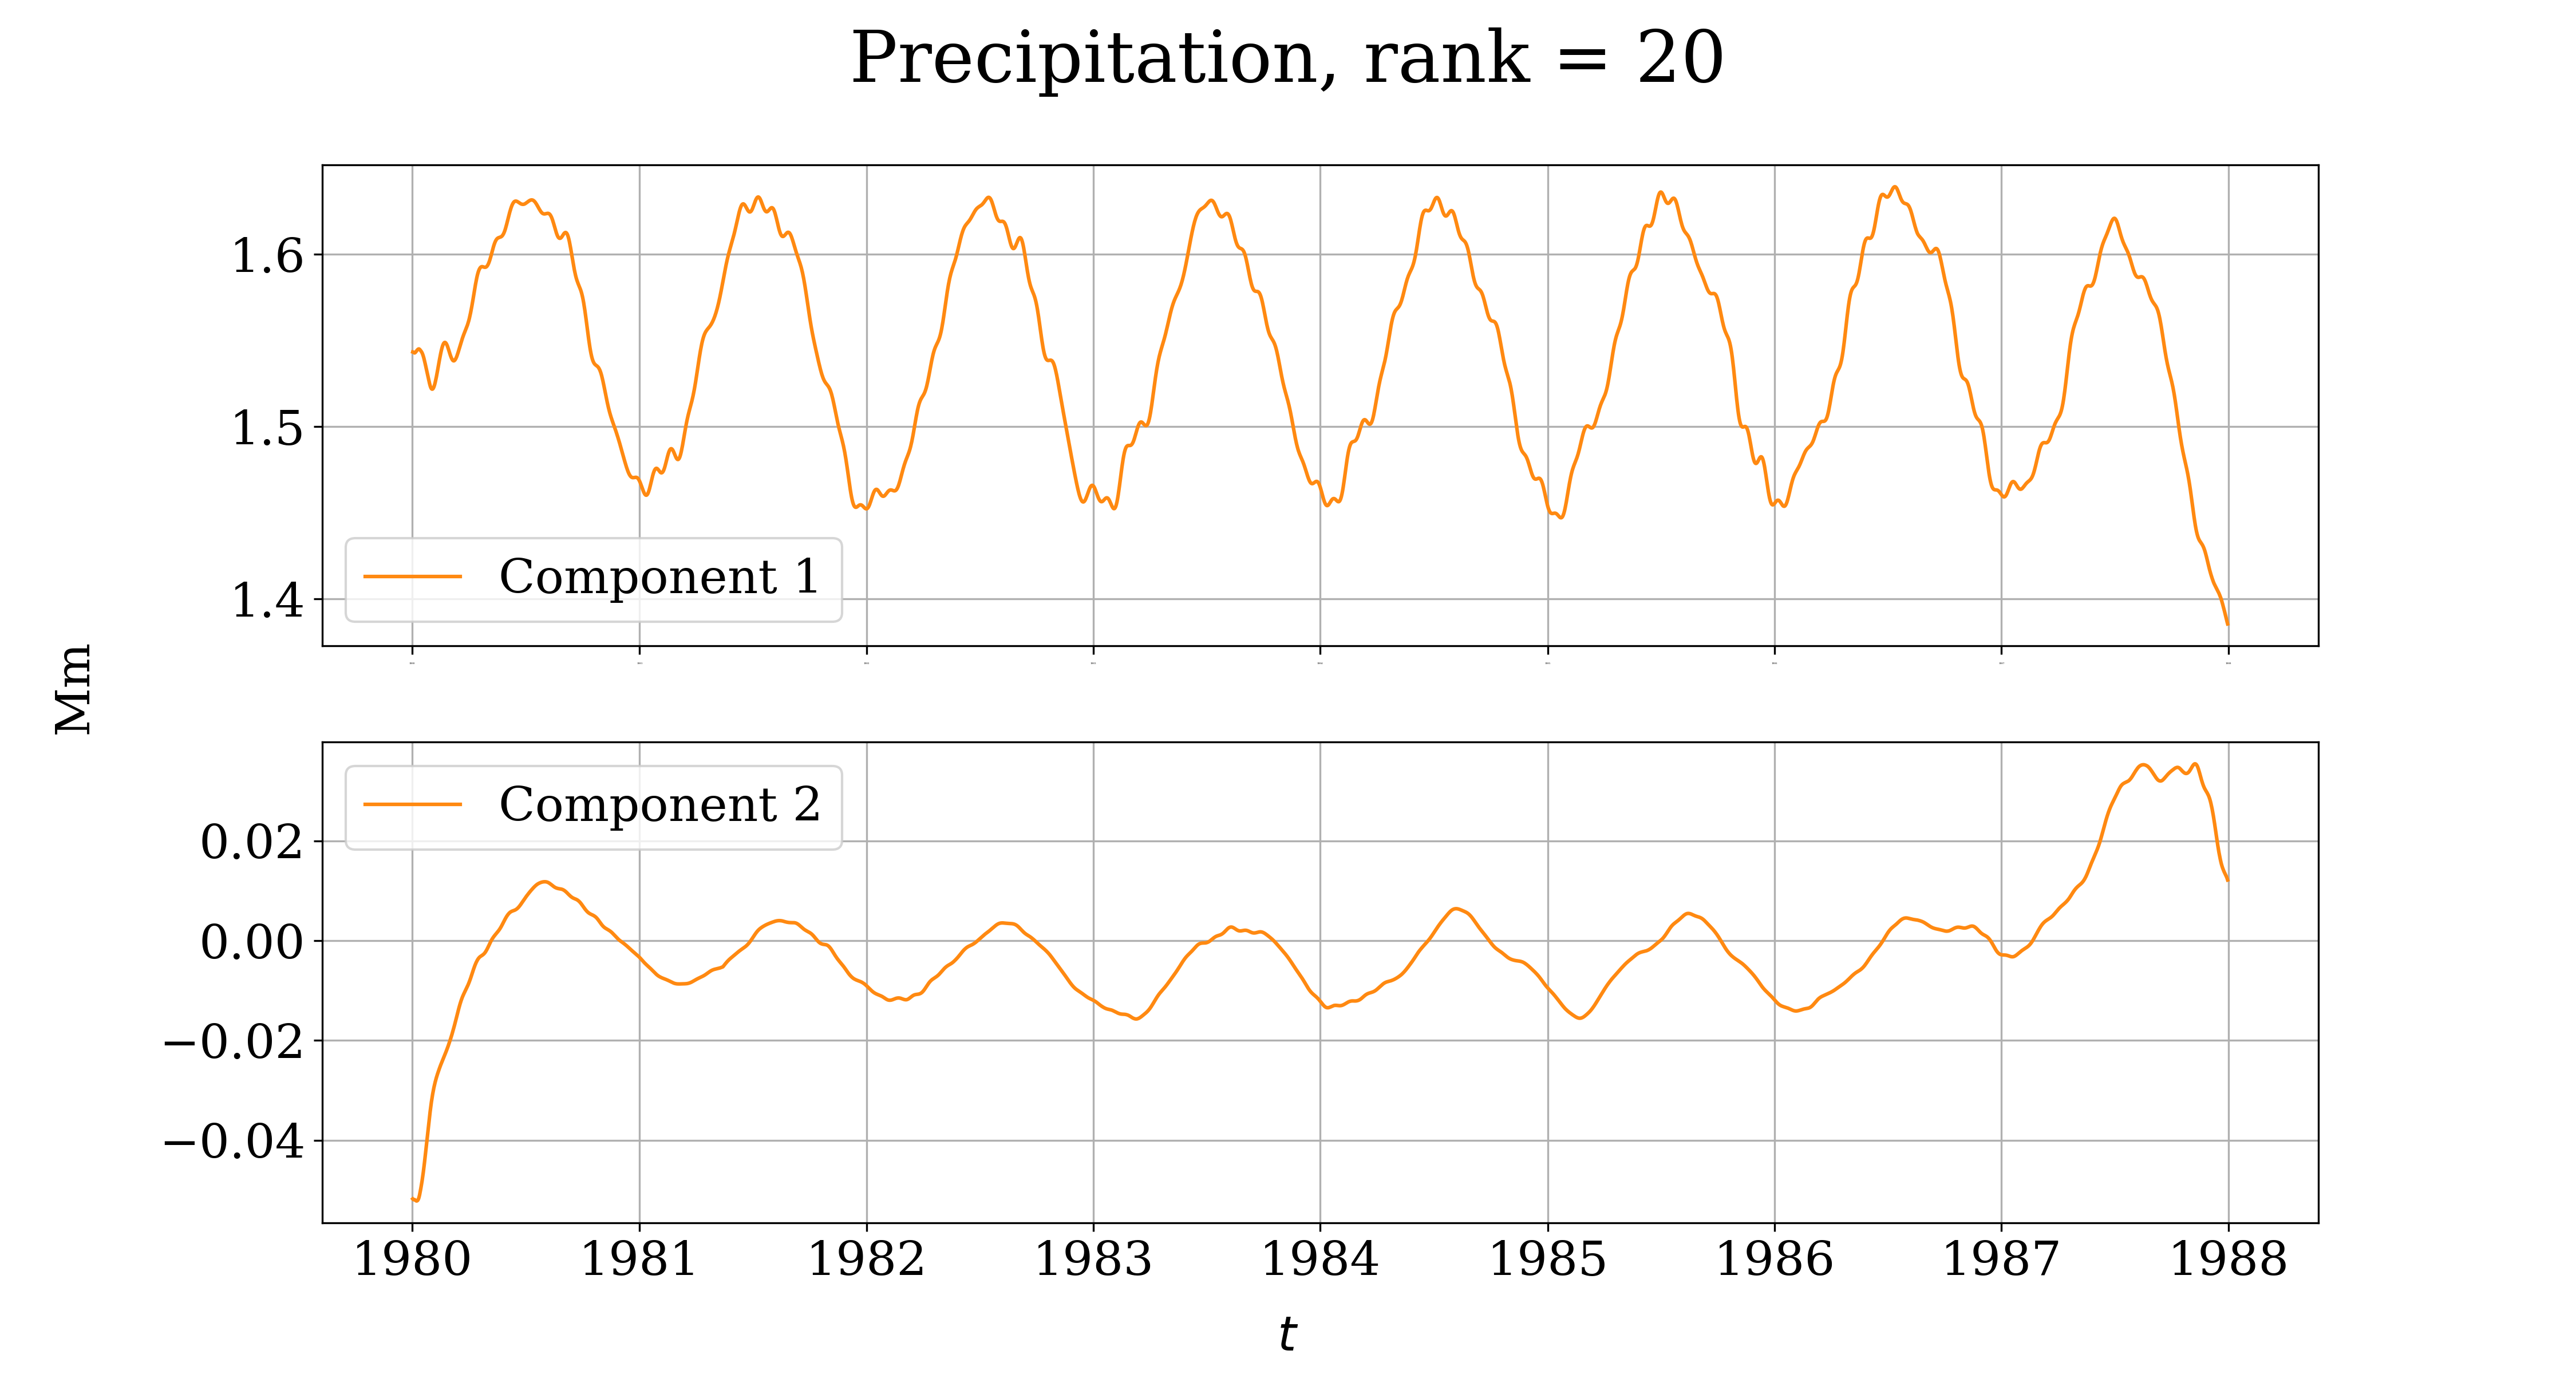
\includegraphics[width=0.48\textwidth, keepaspectratio]{../../experiments/weather/tssa/figs/decomposition/cpd_rank_20/Precipitation.png}
			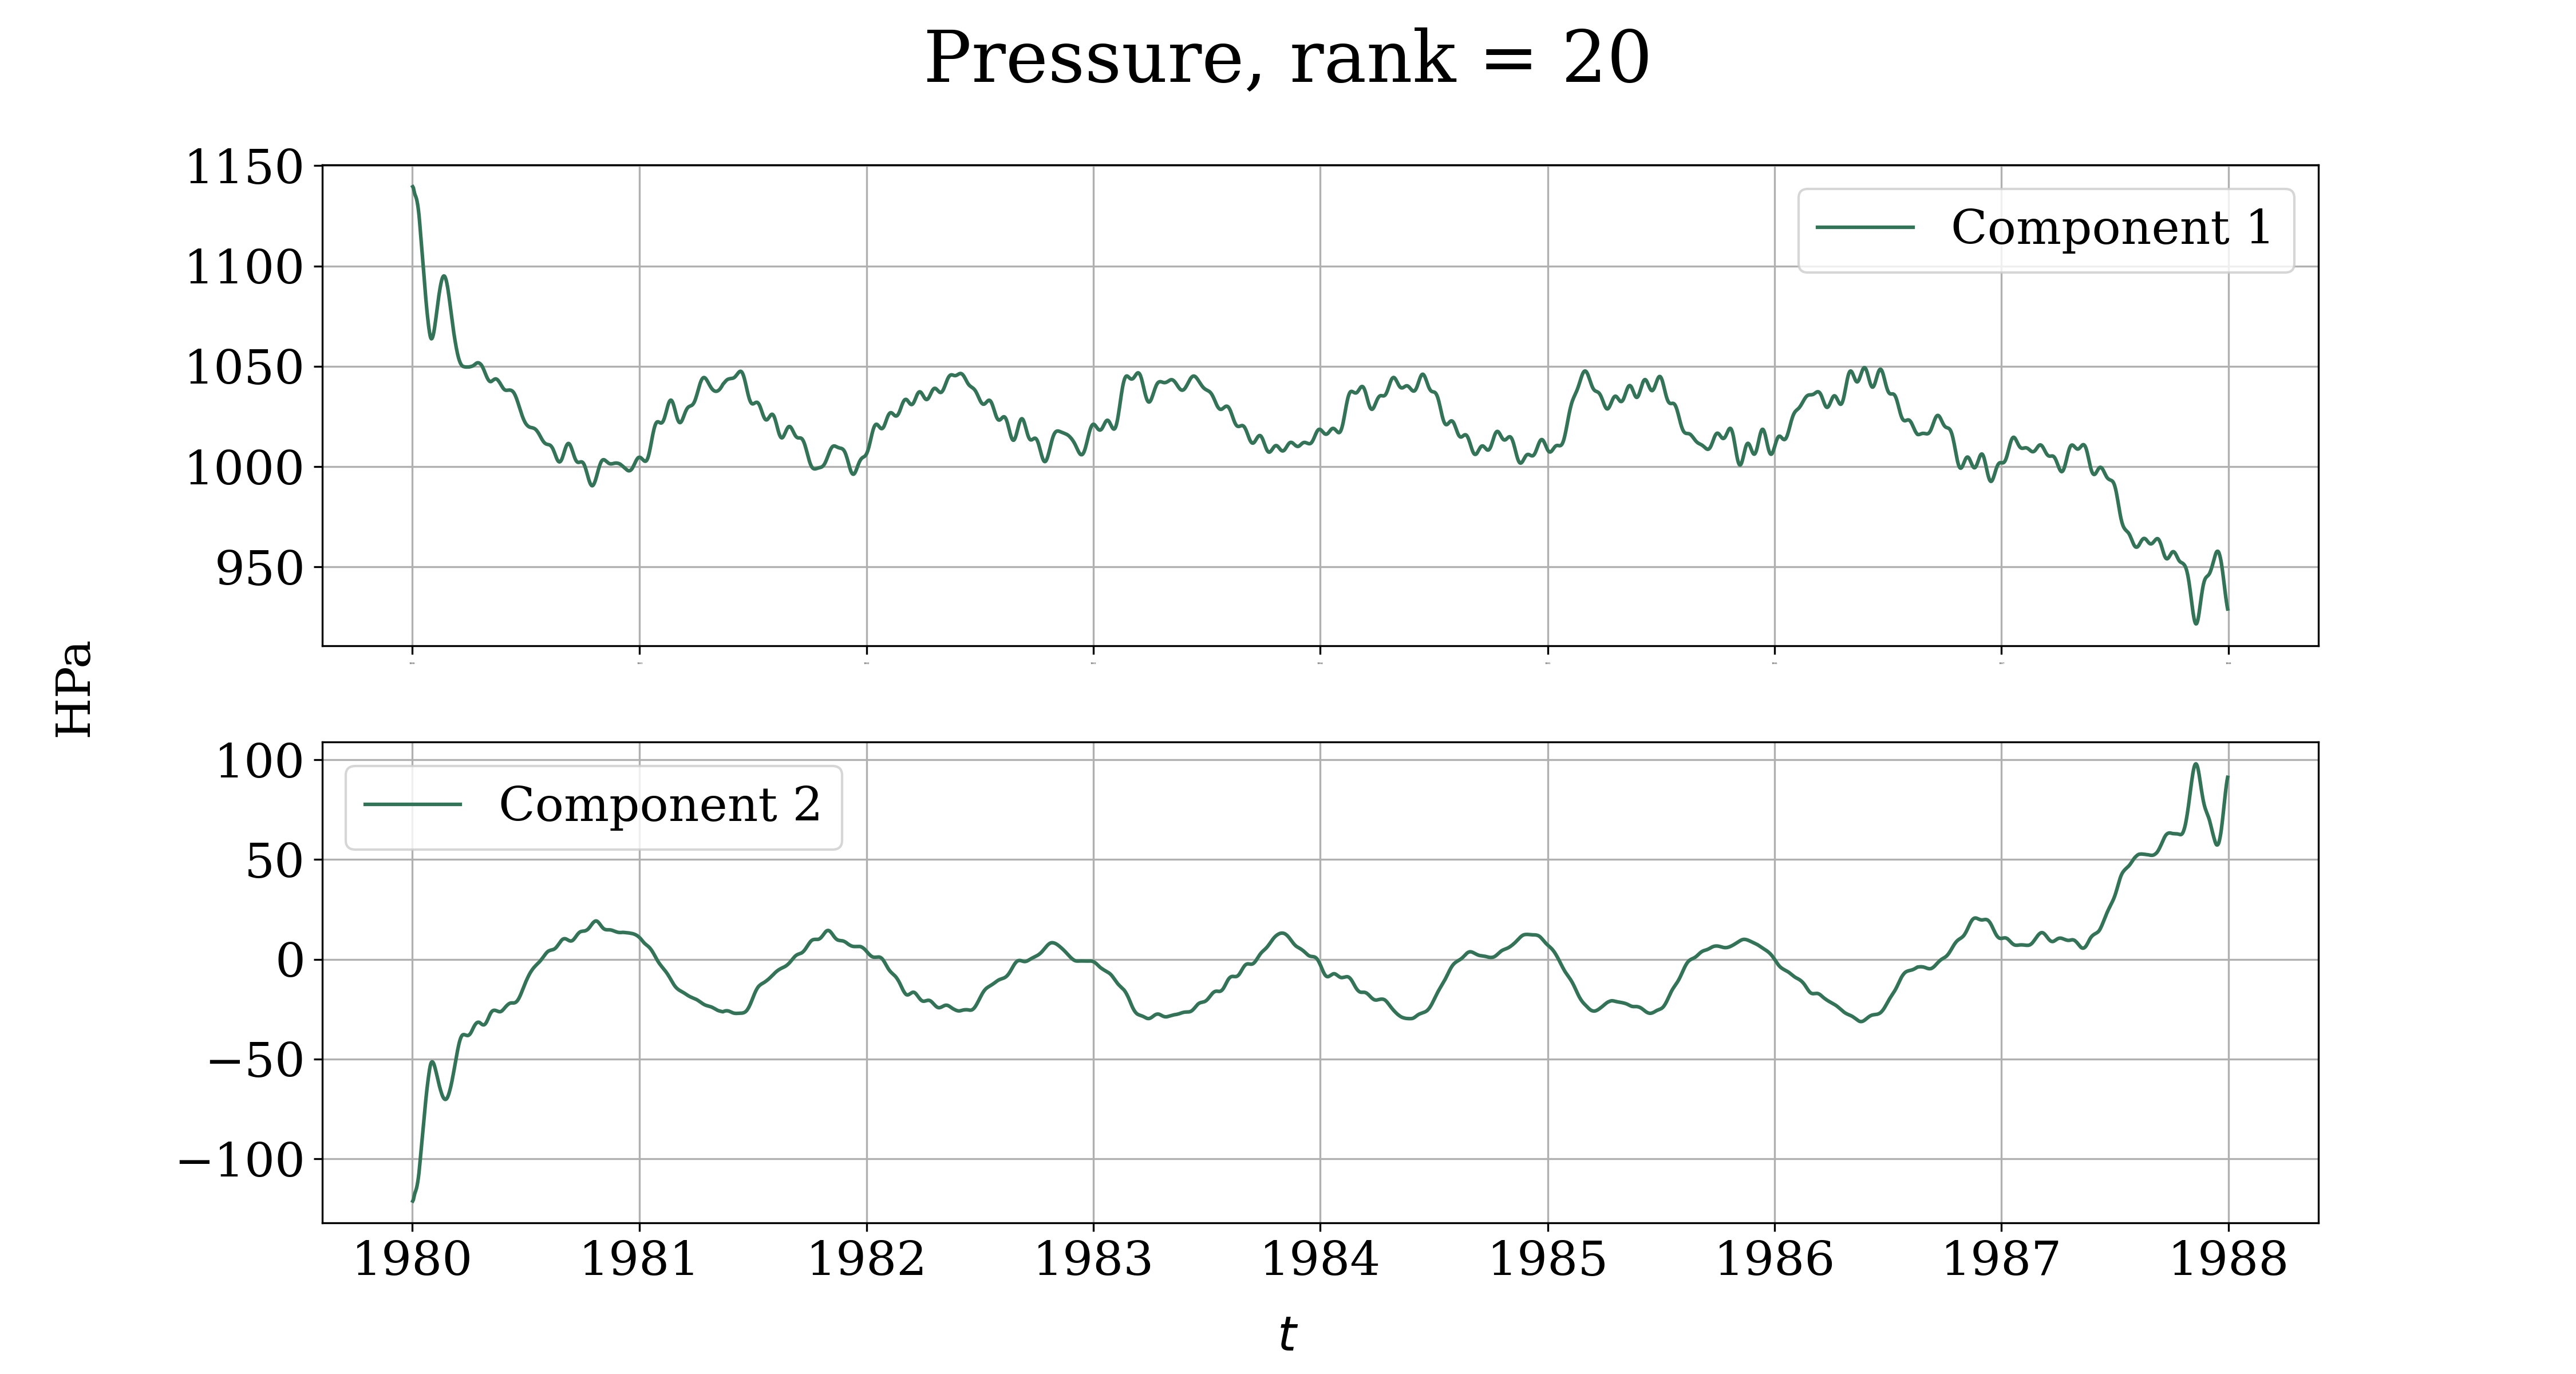
\includegraphics[width=0.48\textwidth, keepaspectratio]{../../experiments/weather/tssa/figs/decomposition/cpd_rank_20/Pressure.png}
			\caption{tSSA decomposition for weather data. CPD rank $ = 20 $}\label{fig:weather_decomp_tssa}
		\end{figure}
		
		
		\begin{figure}[h]
			\centering
			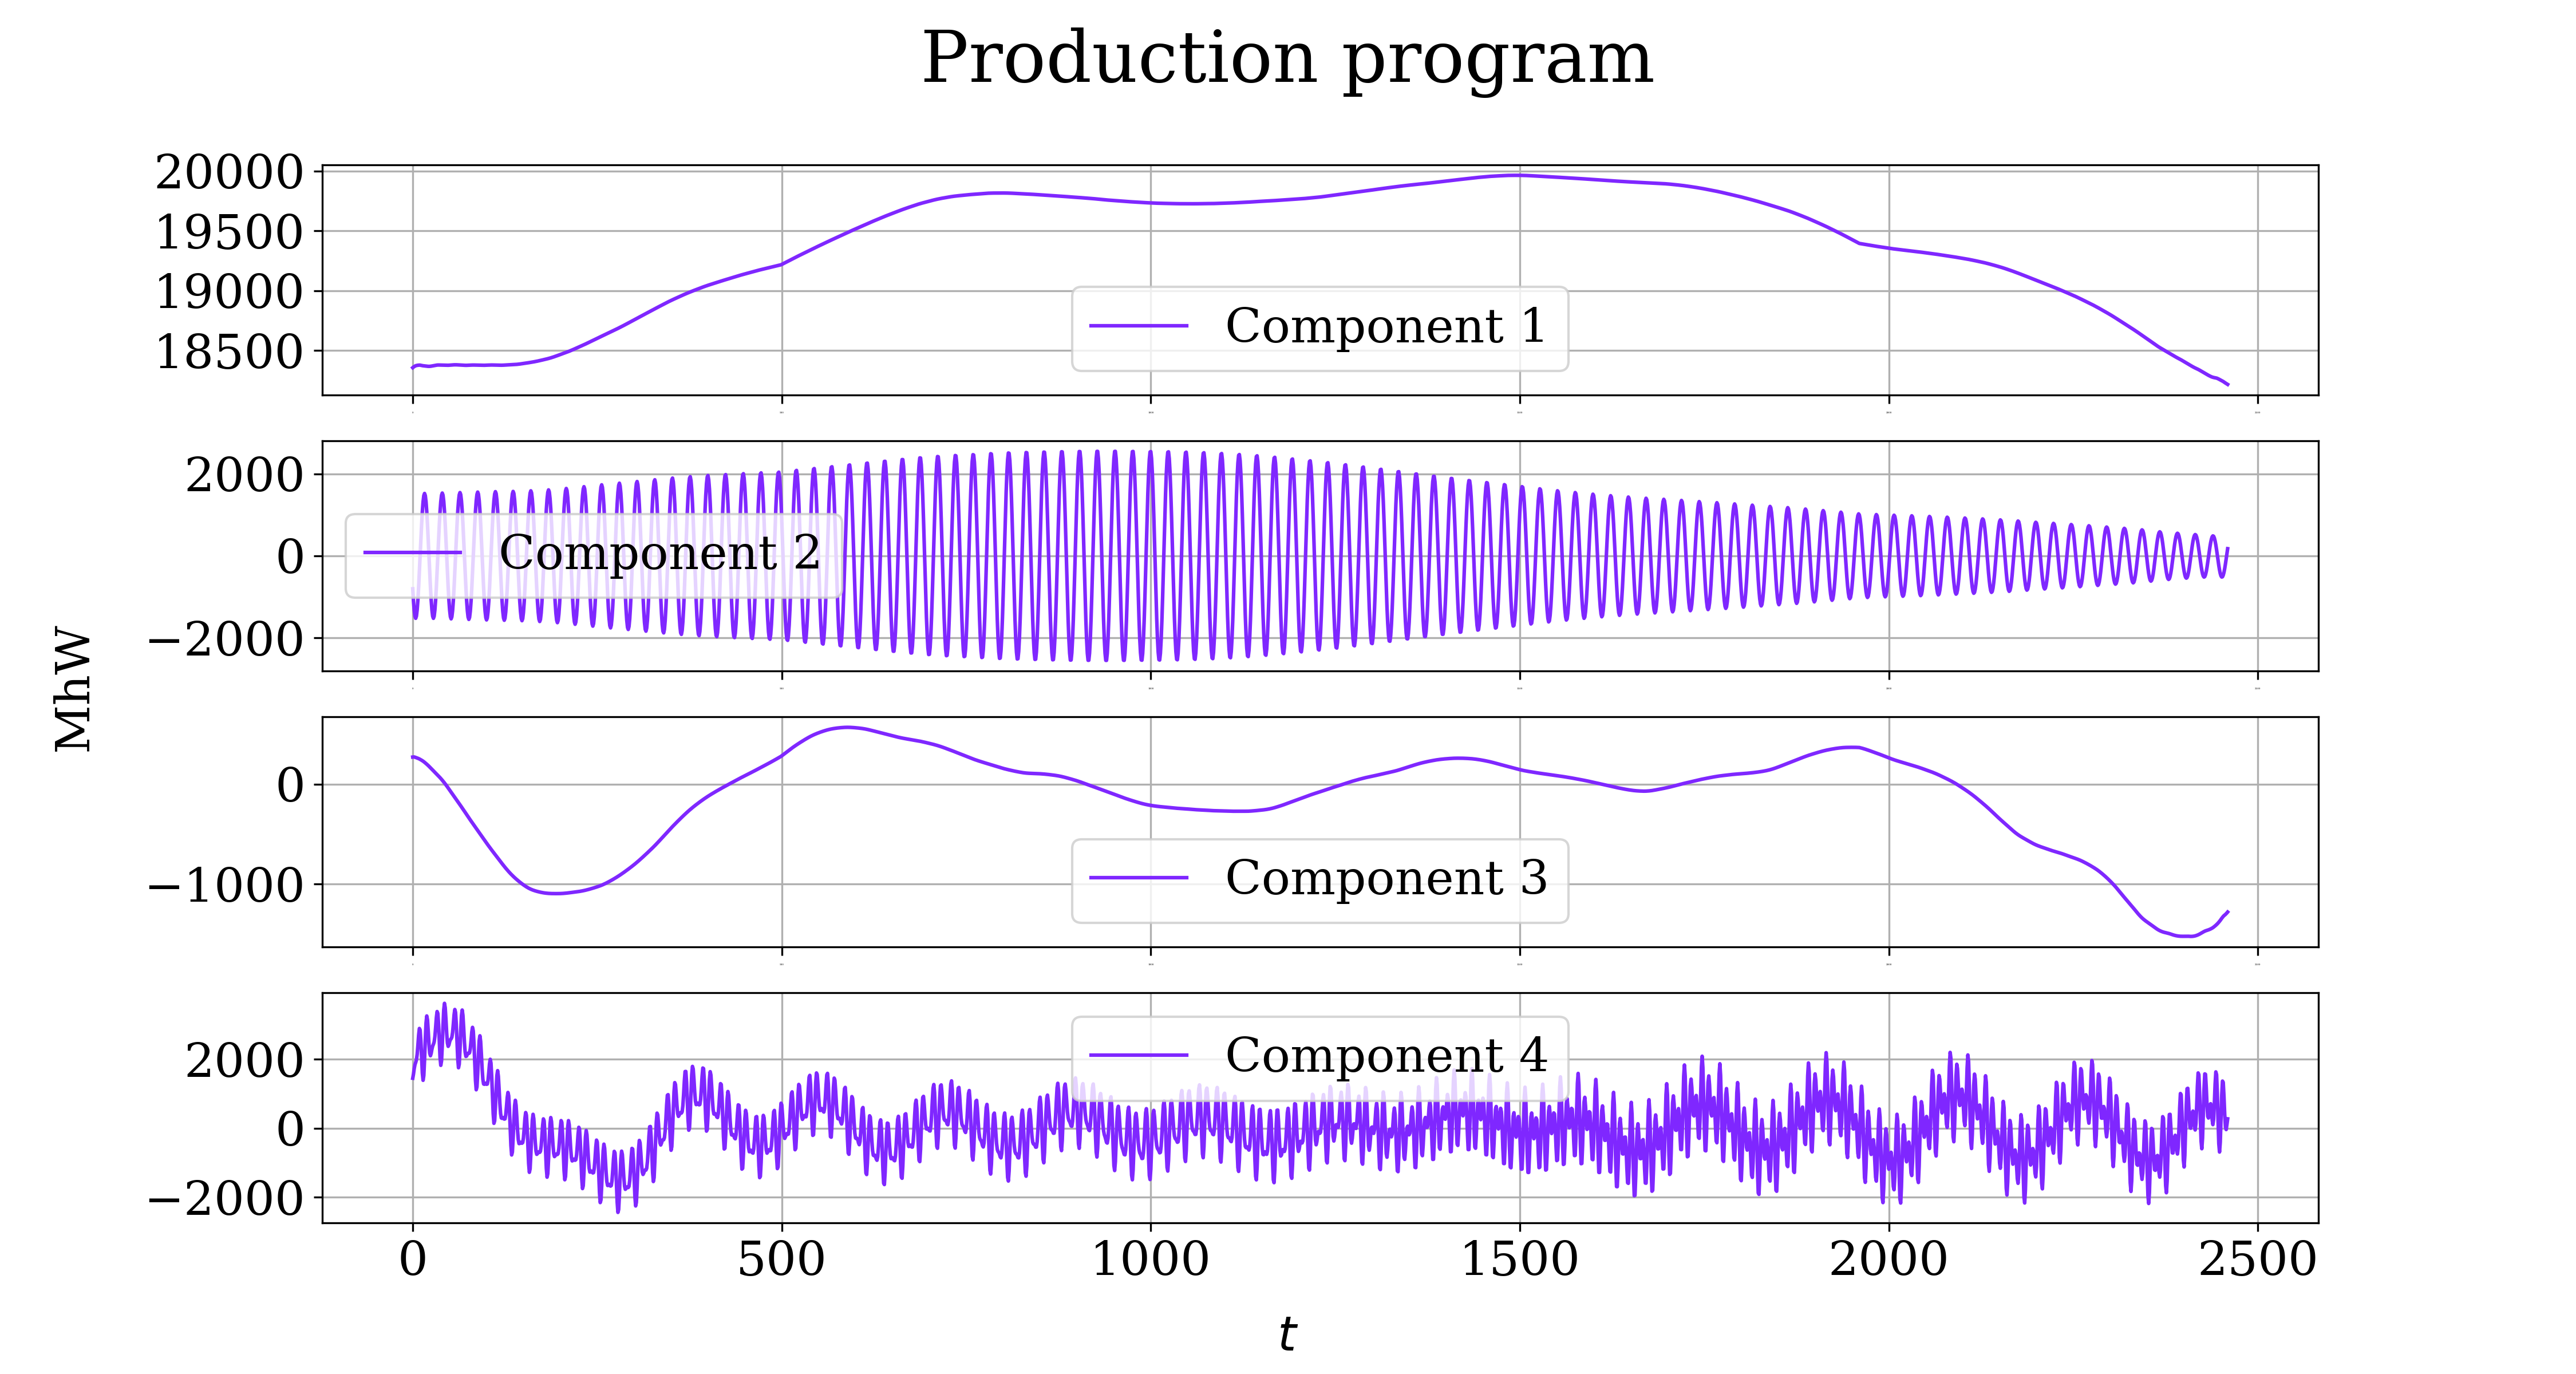
\includegraphics[width=0.48\textwidth, keepaspectratio]{../../experiments/electricity/mssa/figs/decomposition/manual/grouping_1/Production_program.png}
			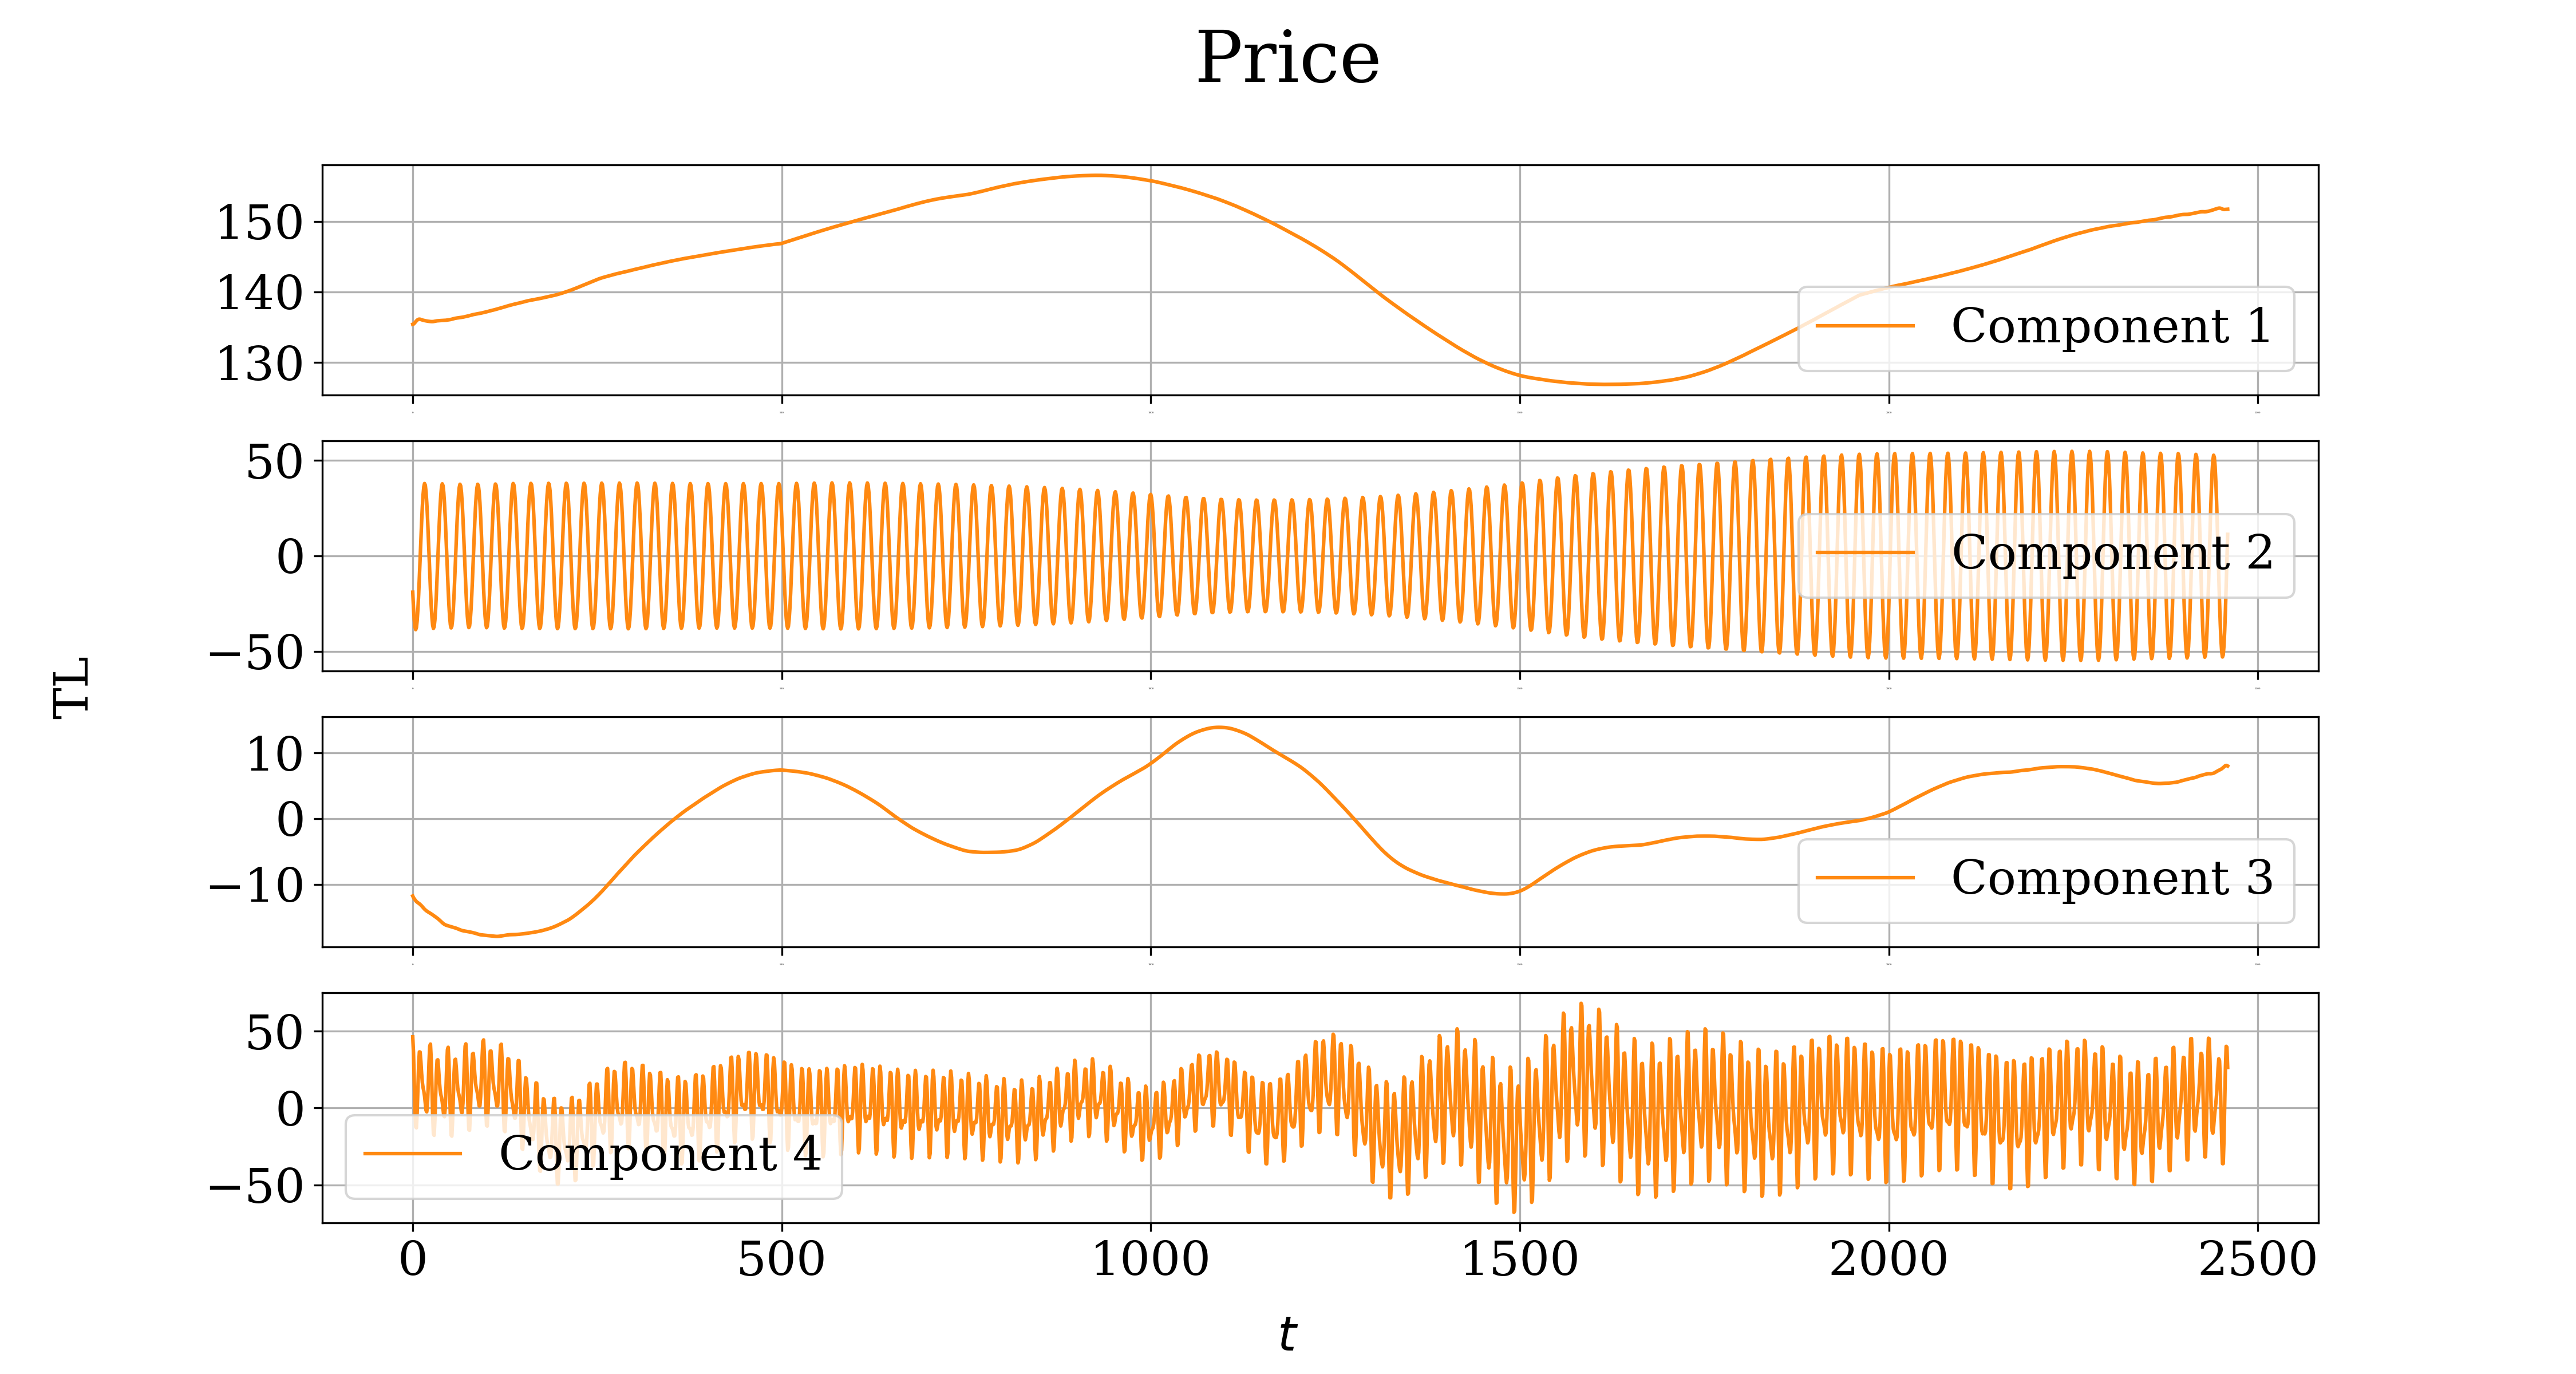
\includegraphics[width=0.48\textwidth, keepaspectratio]{../../experiments/electricity/mssa/figs/decomposition/manual/grouping_1/Price.png}
			\caption{mSSA decomposition for electricity data}\label{fig:electr_decomp_mssa}
		\end{figure}
		
		\begin{figure}[h]
			\centering
			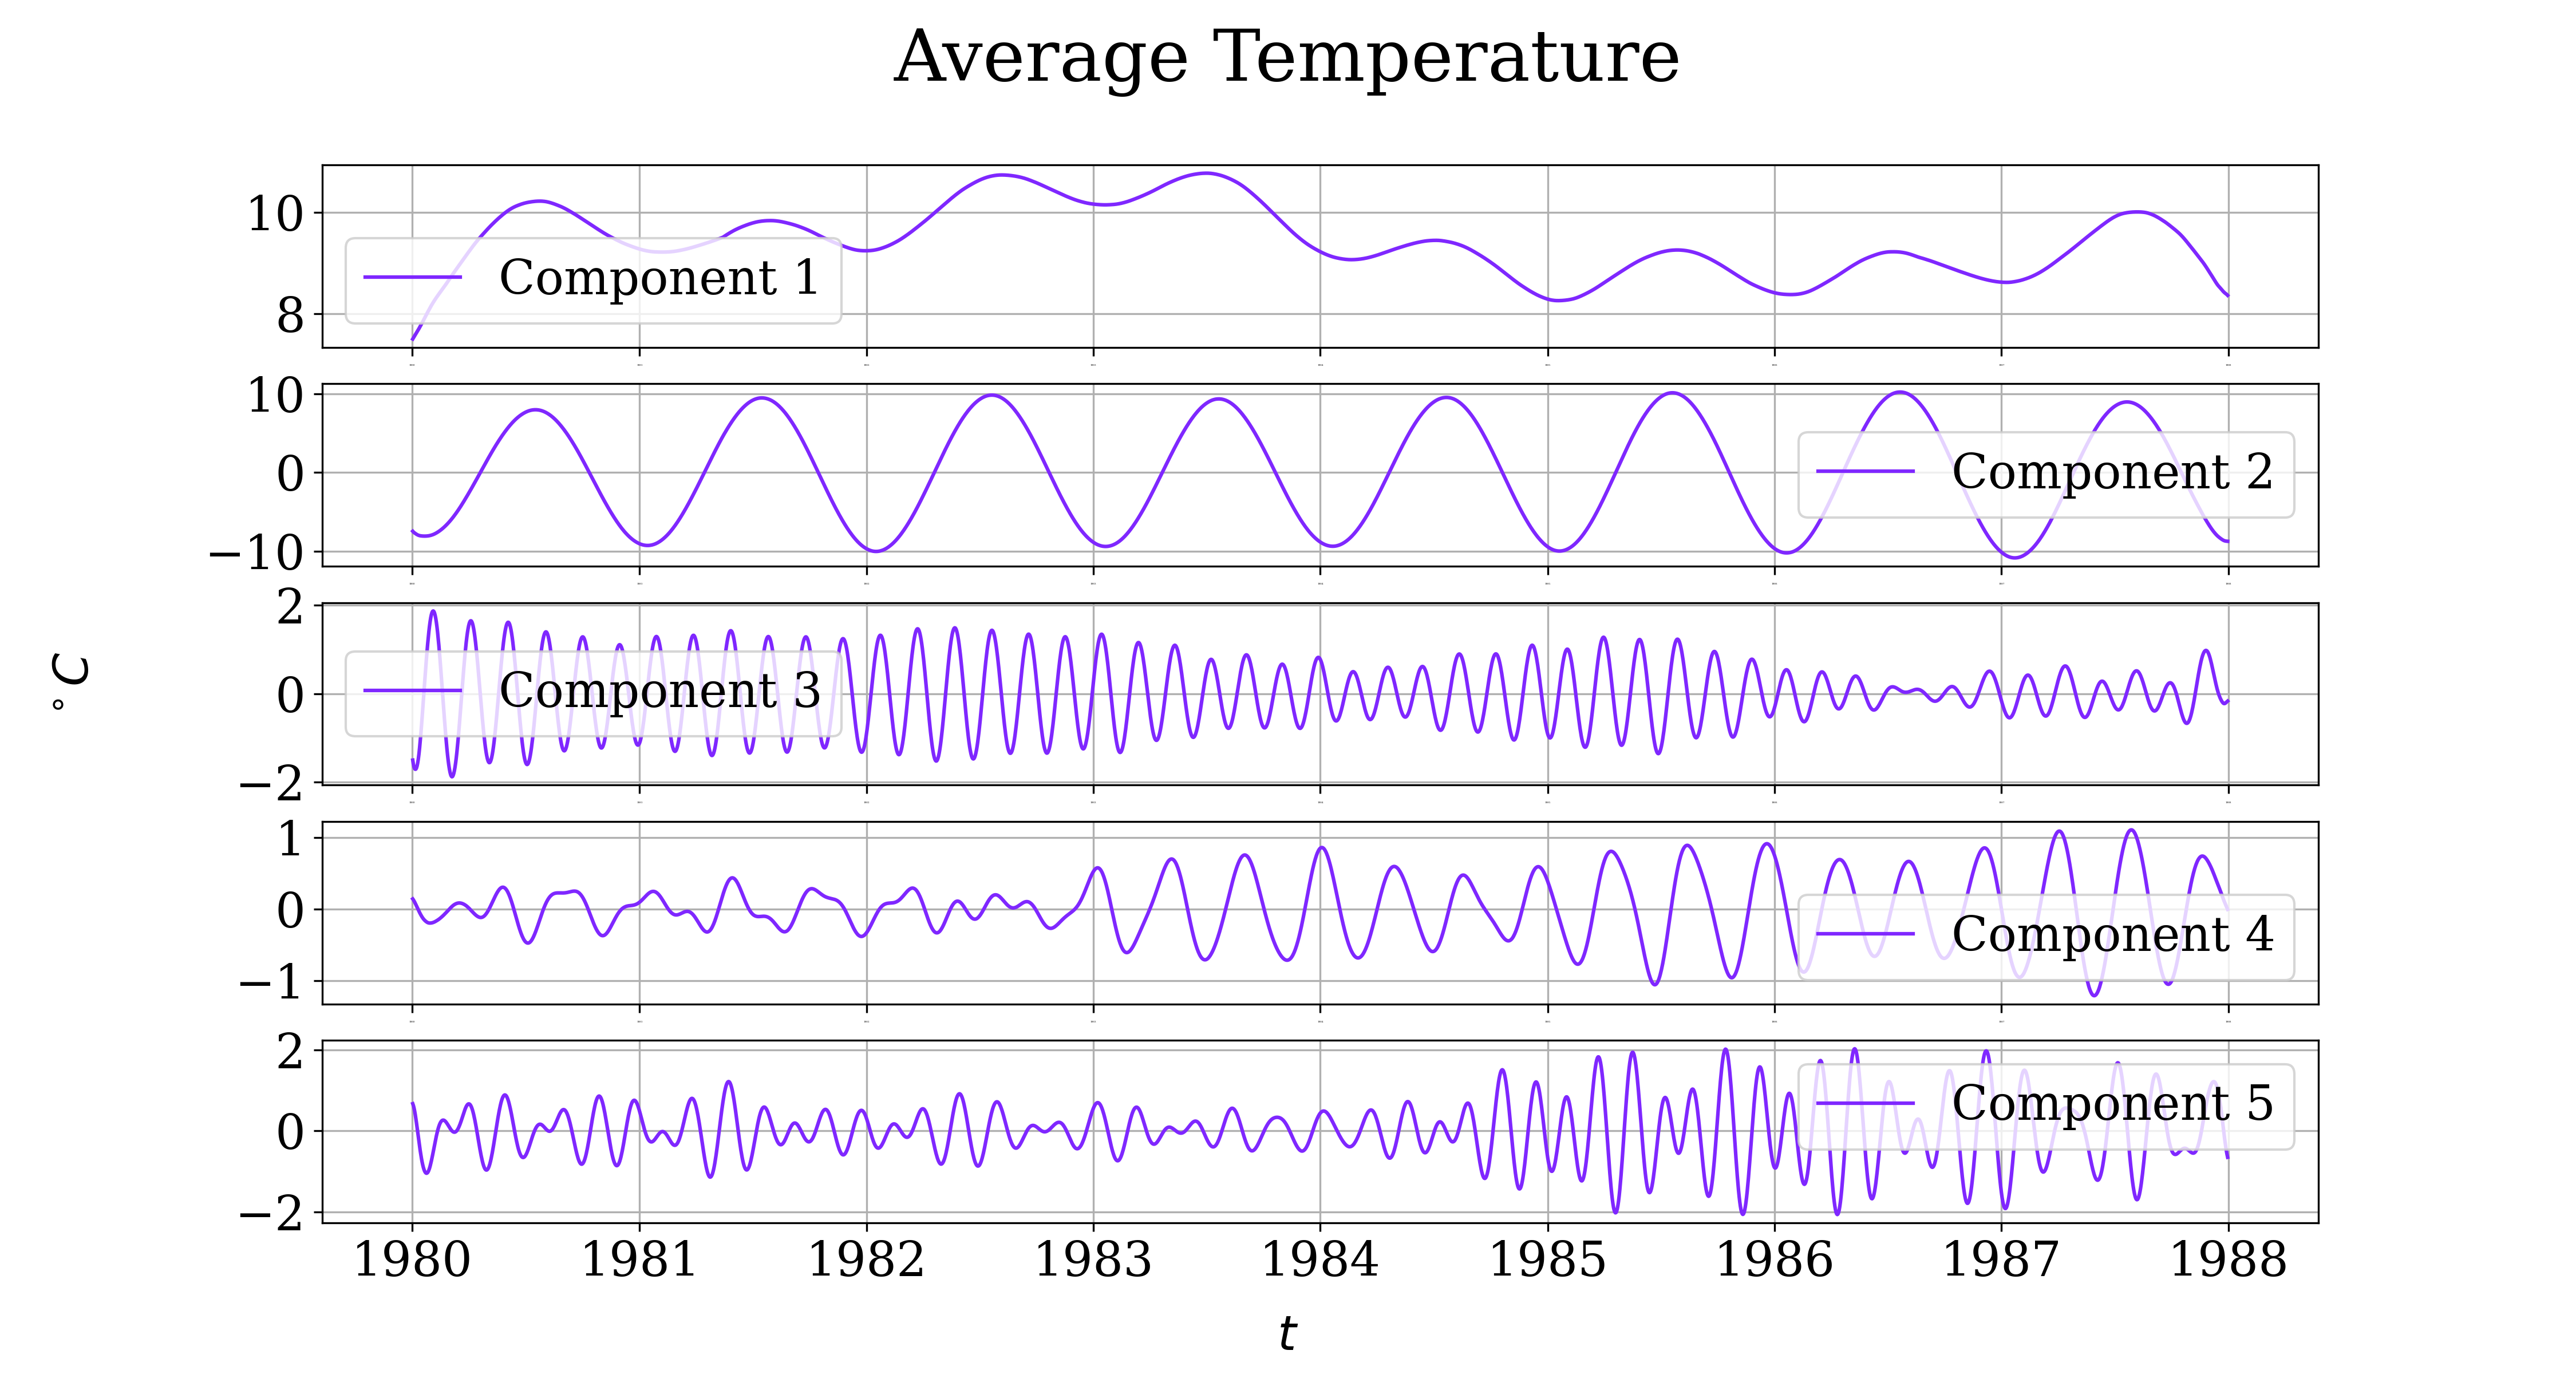
\includegraphics[width=0.48\textwidth, keepaspectratio]{../../experiments/weather/mssa/figs/decomposition/manual/grouping_1/Average_Temperature.png}
			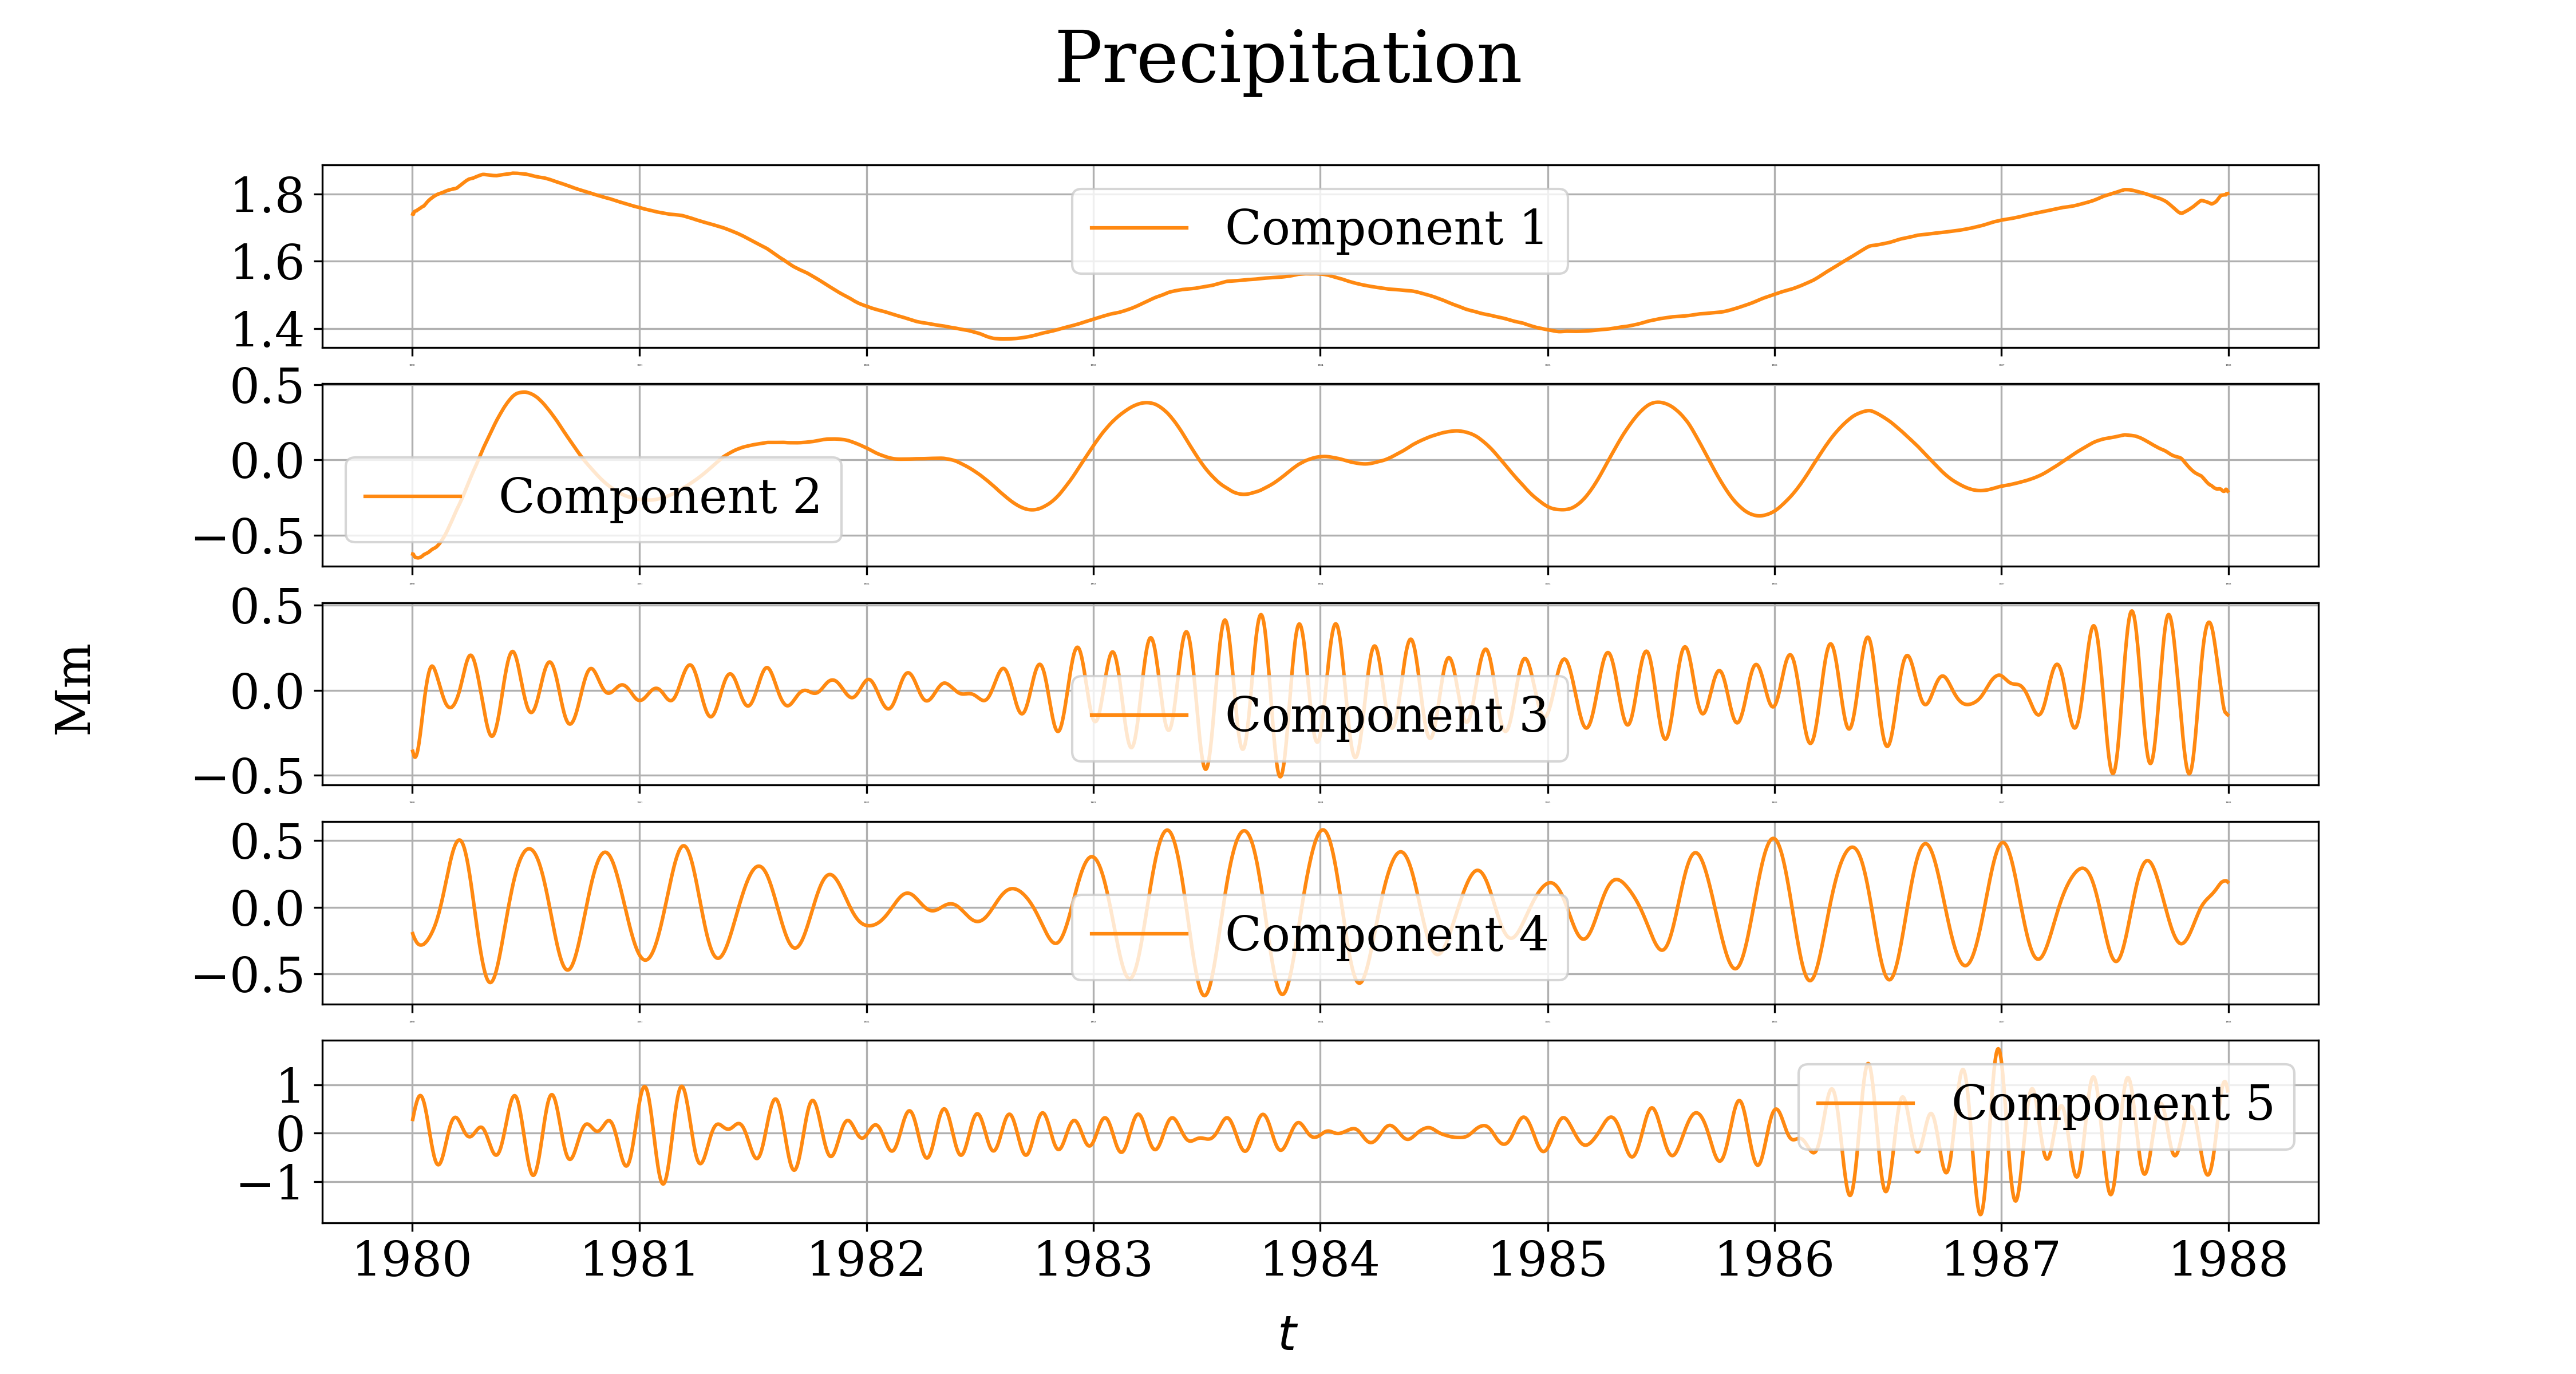
\includegraphics[width=0.48\textwidth, keepaspectratio]{../../experiments/weather/mssa/figs/decomposition/manual/grouping_1/Precipitation.png}
			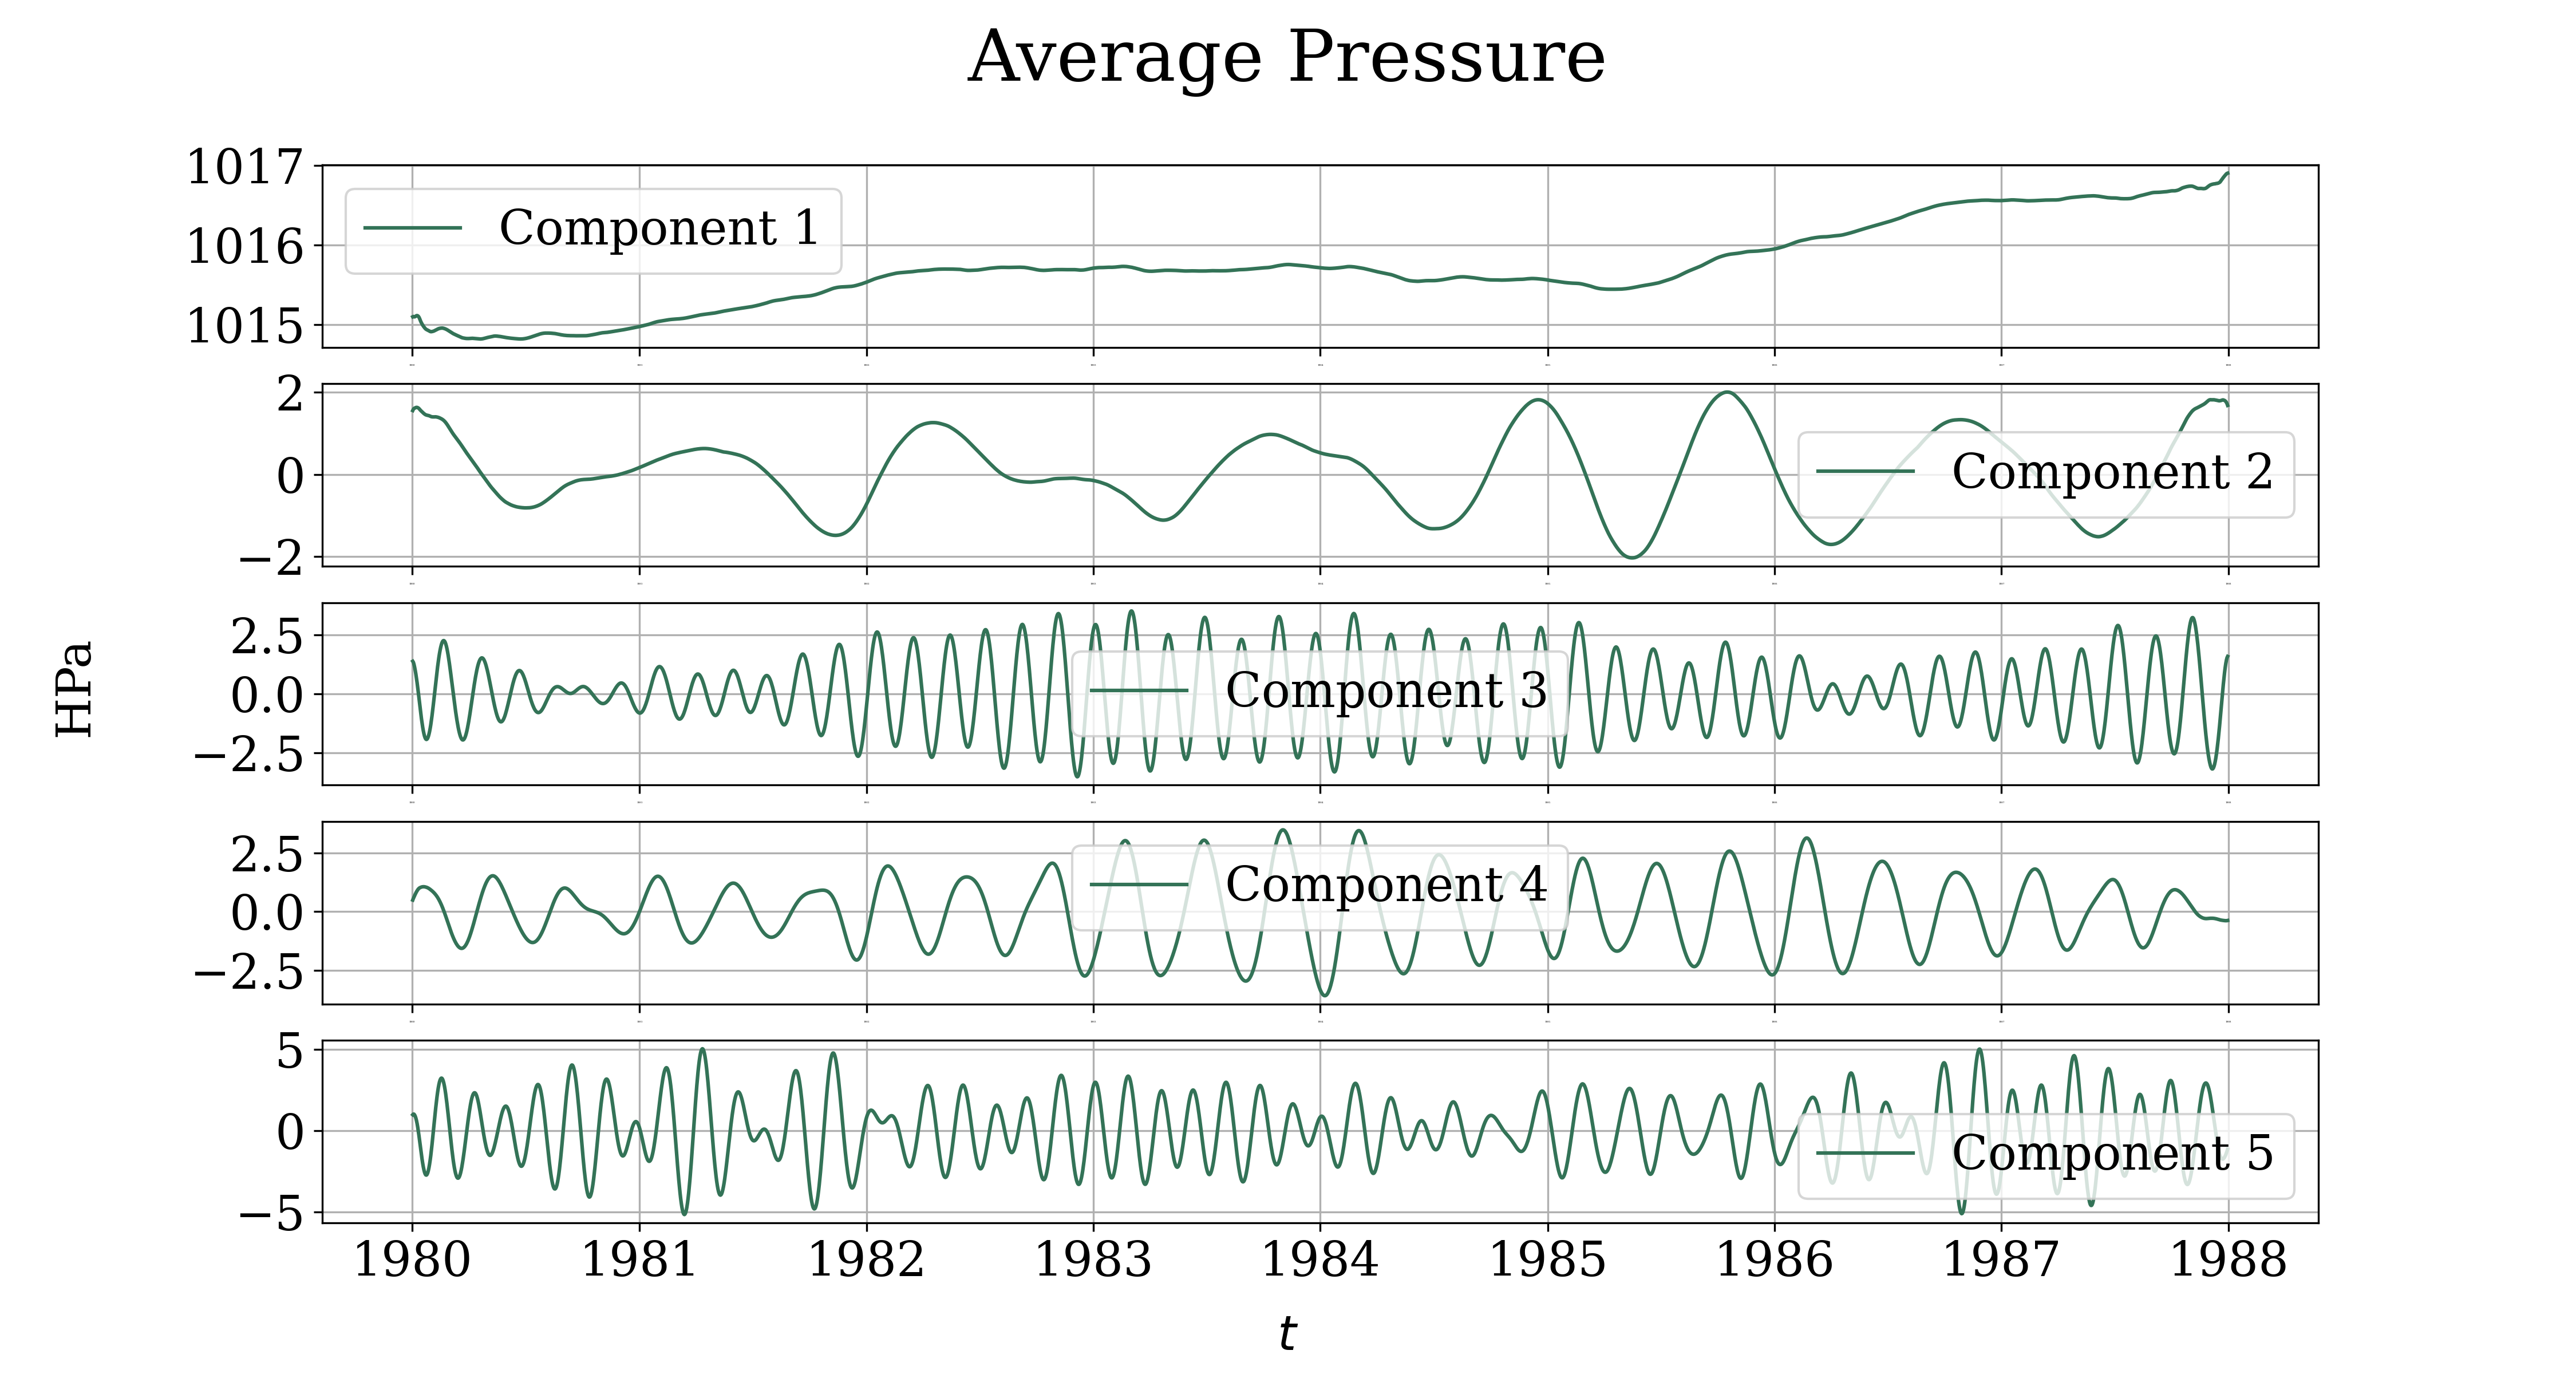
\includegraphics[width=0.48\textwidth, keepaspectratio]{../../experiments/weather/mssa/figs/decomposition/manual/grouping_1/Average_Pressure.png}
			\caption{mSSA decomposition for weather data}\label{fig:weather_decomp_mssa}
		\end{figure}
		
		\clearpage
		\printbibliography
	
 \end{document}